\documentclass[12pt]{extarticle}

%%%% paramètres généraux
%%%% french character
\usepackage[french]{babel}
\usepackage[T1]{fontenc}
\usepackage[utf8]{inputenc}

%%%% useful packages
\usepackage[a4paper, left=1.3cm, right=1.3cm, top=2.2cm, bottom=2.3cm]{geometry}
\usepackage{subcaption} % for figure caption
\usepackage{graphicx} % image
\usepackage{tabularx} % table
\usepackage{lastpage} %pour la définition de la dernière page
\usepackage[table]{xcolor} % color in table
\usepackage{amsmath} % math
\usepackage{amssymb} % bold math
\usepackage{wasysym} % integral
\usepackage[many]{tcolorbox} % colored box
\usepackage{awesomebox} % pour des box déjà définies
\usepackage{fancyhdr} % headers
\usepackage{enumitem} % for bullet in itemize
\usepackage[colorlinks=true,linkcolor=black,citecolor=black,filecolor=black,urlcolor=black]{hyperref} % for link
\usepackage[backend=biber,style=alphabetic,sorting=ynt]{biblatex}
\usepackage{accents} % for complex notation
\usepackage[european, straightvoltages, RPvoltages]{circuitikz} % for electronic circuit

\usepackage{hyperref}   %pour les liens url et les références
\hypersetup{
    colorlinks=true,
    urlcolor=blue,
    linkcolor=blue,
    breaklinks=true
}
\usepackage{empheq}
\usepackage{multicol} % to use several columns
%\setlength{\columnseprule}{1pt} %Separator ruler width
\usepackage{cellspace}  % espace du texte dans les colonnes tableaux
\usepackage{colortbl}  %pour colorier les cases de tableaux
\tcbuselibrary{skins} %library de 
\usepackage{shadow}
\usepackage{pifont}

\usepackage{fontawesome5}

%\usepackage{fontawesome} % awesome icons
\usepackage{ifthen} % for loop and boolean in commands
\usepackage{qrcode}
\usepackage{pdfpages} % to include pdf
\usepackage{wrapfig} % to wrap text around figures
\usepackage{chemfig} % to draw chemistry formula
\usepackage{chemist} % surtout pour chemform
\usepackage{multirow} % for vertically merged cells
\usepackage{makecell} % to format cell in tables
\usepackage{physics} % for derivatives, braket, etc.
\usepackage{esvect} % for large vectors
\usepackage{listings} % for code
\usepackage{dashundergaps} % for automatic text to fill
% dyslexia friendly font (need to be compiled in xetex)
%\usepackage{fontspec}
%\setmainfont{OpenDyslexic}
\usepackage{tikz}
\usepackage{pgfplots}
\usepackage[framemethod=tikz]{mdframed} %pour les boîtes
\usepackage{dashundergaps} %pour les textes à trous

%%%% settings
\setlength{\parskip}{0cm}
\setlength{\parindent}{0cm}
\renewcommand{\baselinestretch}{1.3}
\setcounter{tocdepth}{2}
\renewcommand{\thesection}{\textcolor{red}{\Roman{section}}}
\renewcommand{\thesubsection}{\textcolor{red}{\Roman{section}.\arabic{subsection}}}

%%%% tikz configuration
\usetikzlibrary{babel}
\tikzset{>=latex}
\usetikzlibrary{shadows}
\usetikzlibrary{backgrounds}



%%%% header
\renewcommand{\headrulewidth}{0.4pt}
\setlength{\headheight}{22.50113pt}


%%%% Table
\renewcommand{\tabularxcolumn}[1]{m{#1}}
\setlength{\extrarowheight}{8pt}
\newcolumntype{P}[1]{>{\centering\arraybackslash}p{#1\linewidth}}% colonne de type p mais centrée
\cellspacetoplimit 2pt %espace au dessus du texte
\cellspacebottomlimit 2pt  %espace en dessous du texte



%%%% Chemfig configuration
\setchemfig{
  atom sep=20pt,
  bond style={line width=1pt},
  angle increment=30
}


%%%% dashundergaps configuration
\dashundergapssetup{
  gap-numbers = false,
  gap-format = dot,
  gap-widen,
  gap-extend-percent
}


%\bibliographystyle{plain}
\bibliography{TSNR/TSNR.bib}

%%%% quelques commandes
%%%%%%%%%%%%%%%%%%%%%%%%%%%%%%%%%%%%%%%%%%%%%%%%%%%%%%%%%%%%%%%%%%%%%%%%%%
%%%% quelque couleurs
\definecolor{vertSombre} {RGB}{  0,  92,  46}
\definecolor{cyanSombre} {RGB}{  0, 140, 128}
\definecolor{jauneSombre}{RGB}{138, 103,   0}
\definecolor{jauneClair} {RGB}{218, 173,   0}
\definecolor{rougeSombre}{RGB}{148,  31,   0}
\definecolor{rougeClair} {RGB}{224,  39,  34}
\definecolor{couleurtitre}{RGB}{255,  255,  255}
\definecolor{exef}{RGB}{210,210,210}
\definecolor{propositiono}{RGB}{109,109,109}

%%% quelques couleurs dérivées des couleurs choisie
\newcommand{\couleurCorrection}{couleurPrincipale!60!black}
\newcommand{\couleurExercice}{couleurPrincipale!75!black}

%%%% rectangle coloré
\newcommand\rectangle[3]{%
  \shorthandoff{;}
  \tikz \node (rect) [draw, fill, color=#1,
              minimum width=#2,
              minimum height=#3] {};
  \shorthandon{;}
}
\newcommand\rectangleCyan[2]{\rectangle{couleurPrincipale}{#1}{#2}}

%%%% simple boite
\newenvironment{boite}{
  \begin{tcolorbox}
  [ breakable, enhanced jigsaw, % to break box over page
    arc = 0mm, % straight line
    colback= white, % white background
    colframe= black % dark frame
  ]
}
{ \end{tcolorbox} }

\newtcolorbox{facile}[2][]{colback=green!5!white,
colframe=green!75!black,fonttitle=\bfseries,
colbacktitle=green!85!black,enhanced,
attach boxed title to top center={yshift=-2mm},
title={#2},#1}

\newtcolorbox{difficile}[2][]{colback=red!5!white,
colframe=red!75!black,fonttitle=\bfseries,
colbacktitle=red!85!black,enhanced,
attach boxed title to top center={yshift=-2mm},
title={#2},#1}


%\newenvironment[1]{Propriete}{\begin{tcolorbox}[colback=red!5!white,colframe=red!75!black,title=\textbf{#1 :}]
%}
%{\end{tcolorbox} 


%%%%%%%%%%%%%%%%%%%%%%%%%%%%%%%%%%%%%%%%%%%%%%%%%%%%%%%%%%%%%%%%%%%%%%%%%%
%%%% pagination et sections
\newcommand{\titre}[1]{
  \begin{center}
    \textsf{\bfseries \Large #1}
  \end{center}
}
\newcommand{\sousTitre}[1]{
  \textsf{\bfseries #1}
}
\newcommand{\pasDePagination}{
  \thispagestyle{empty}
}
\newcommand{\feuilleBlanche}{
  \newpage
  \phantom{b}
  \pasDePagination
}


%%%% activité ou TP
\newcounter{acti}
\newcommand{\titreActi}[2]{
  \refstepcounter{acti}
  \titre{#1 \arabic{section}.\arabic{acti} -- #2}
}
\newcommand{\titreTP}[1]{
  \titreActi{TP}{#1}
  %\titreActi{Activité expérimentale}{#1}
}
\newcommand{\titreActivite}[1]{
  \titreActi{Activité}{#1}
}
\newcommand{\titreEvaluation}[1]{
  \titreActi{Évaluation}{#1}
}


%%%% chapitre, section et sous-section
\newcommand{\titreChapitre}[1]{
  \titre{Chapitre \arabic{section} : #1}
}
\newcommand{\titrePartie}[1]{
  \vspace*{24pt}
  \refstepcounter{subsection}
  \rectangleCyan{60pt}{1pt}
  \sousTitre{\Large \Roman{subsection} -- #1}
  \rectangleCyan{60pt}{1pt}
  \vspace*{10pt}
}
\newcounter{sousSection}
\newcommand{\titreSection}[1]{
  \vspace*{16pt}
  \refstepcounter{subsubsection}
  \setcounter{sousSection}{0}
  \rectangleCyan{30pt}{4pt}
  \sousTitre{\large \arabic{subsubsection} -- #1}
  \vspace*{10pt}
}
\newcommand{\titreSousSection}[1]{
  \vspace*{12pt}
  \refstepcounter{sousSection}
  \sousTitre{\Alph{sousSection} -- #1}
  \vspace*{8pt}
}

%%%% fixe le numéro de l'activité
\newcommand{\numeroActivite}[1]{
  \setcounter{subsection}{0}
  \setcounter{subsubsection}{0}
  \setcounter{sousSection}{0}
  \setcounter{figure}{0}
  \setcounter{document}{0}
  \setcounter{exercice}{0}
  \setcounter{QCM}{0}
  \setcounter{countCoupDePouce}{0}
  \setcounter{acti}{#1 - 1}
  \setcounter{page}{1}
}
% fixe le numéro de page (#2) et de partie (#1)
\newcommand{\numeroPartieCours}[2]{
  \newpage
  \setcounter{subsection}{#1 - 1}
  \setcounter{page}{#2}
}

%%%% lignes
\newcommand{\ligne}{
  \par\noindent\rule{\textwidth}{0.4pt}
}
\newcommand{\lignePointillee}[1]{
  \makebox[#1\textwidth]{\dotfill}
}


%%%%%%%%%%%%%%%%%%%%%%%%%%%%%%%%%%%%%%%%%%%%%%%%%%%%%%%%%%%%%%%%%%%%%%%%%%
%%%% en-tête
\newcommand{\teteGauche}[1]{
  \lhead{
    \textbf{\footnotesize #1}
  }
}
\newcommand{\teteDroite}[1]{
  \rhead{
    \hfill \textbf{\footnotesize #1}
  }
}

%

\newcommand{\enTeteRevision}[2]{
  \pagestyle{fancy}
  \lhead{Revision #1 - \textit{#2}}
  %\chead{} % central header
  \teteDroite{Lycée Parc de Vilgénis 2023 - 2024}
}

\newcommand{\enTeteExercice}[1]{
  \pagestyle{fancy}
  \lhead{Exercices du Chapitre #1}
  %\chead{} % central header
  \teteDroite{Lycée Parc de Vilgénis 2023 - 2024}
}

\newcommand{\enTeteMethodo}[2]{
  \pagestyle{fancy}
  \teteGauche{Fiche Méthode #1 : #2}
  %\chead{} % central header
  \teteDroite{Lycée Parc de Vilgénis 2023 - 2024}
}

\newcommand{\enTeteChap}[2]{
  \pagestyle{fancy}
  \lhead{Chapitre #1 - \textit{#2}}
  %\chead{} % central header
  \teteDroite{Lycée Parc de Vilgénis 2023 - 2024}
}

\newcommand{\enTeteExo}[1]{
  \pagestyle{fancy}
  \lhead{Exercices du Chapitre #1}
  %\chead{} % central header
  \teteDroite{Lycée Parc de Vilgénis 2023 - 2024}
}

\newcommand{\enTeteAct}[3]{
  \pagestyle{fancy}
  \lhead{Chapitre #1 \newline Activité #2 - \textit{#3}}
  %\chead{} % central header
  \teteDroite{Lycée Parc de Vilgénis 2023 - 2024}
}

\newcommand{\enTeteDM}[2]{
  \pagestyle{fancy}
  \lhead{Devoir Maison n$\degree$ #1 - \textit{#2}}
  %\chead{} % central header
  \teteDroite{Lycée Parc de Vilgénis 2023 - 2024}
}

\newcommand{\enTeteTP}[2]{
  \pagestyle{fancy}
  \lhead{TP #1 - \textit{#2}}
  %\chead{} % central header
  \teteDroite{Lycée Parc de Vilgénis 2023 - 2024}
}
%
\newcommand{\enTeteSeance}[2]{
  \pagestyle{fancy}
  \lhead{Date : \textit{#1}}
  \chead{Séance : #2}
  \teteDroite{Seconde} % central header
}
%

\newcommand{\enTeteFicheReussite}[1]{
  \newpage
  \setcounter{subsection}{0}
  \pasDePagination
  
  \phantom{b}
  \vspace*{-70pt}
  \titre{Fiche \og Réussir son évaluation \fg}
  \titre{#1}
  
  \vspace*{-6pt}
  % \titreSection{Ce que je dois savoir}
  
  Pour savoir quoi réviser, je lis les points clés du chapitre évalués :
  \begin{itemize}
    \item Si je pense maîtriser une notion, je coche la case \ok
    \item Si je pense que je dois la retravailler, je coche la case \pasOk
  \end{itemize}
  
  Pour travailler les notions qui ne sont pas maîtrisées, je reprend les activités associés.
}
\newcommand{\basDePageFicheReussite}{
  \titreSection{Ce qu'il me reste à faire}
}
\newcommand{\travailExerciceCorrige}{
  Pour être sûr-e d'obtenir une bonne note, je m'entraîne avec les exercices corrigés du manuel indiqués dans la colonne de droite.
}
\newcommand{\questionFicheReussite}[1]{
  S'il me reste des questions, je les note ici pour les poser au début de l'évaluation :\\[4pt]
  \lignesReponse{#1}
}
\newcommand{\coursFicheReussite}{
  Je prépare une fiche au format A4 avec toutes les notions, définitions ou grandeurs dont je pense avoir besoin pendant l'évaluation.
}


%%%%%%%%%%%%%%%%%%%%%%%%%%%%%%%%%%%%%%%%%%%%%%%%%%%%%%%%%%%%%%%%%%%%%%%%%%
%%%% exercice
% définit un booléen pour entrer ou sortir du mode correction
\newboolean{modeProf}
\setboolean{modeProf}{false}
\newcommand{\modeCorrection}{
  \setboolean{modeProf}{true}
  \TeacherModeOn
}

% définit une commande pour afficher une question 
% #1 : question
% #2 : réponse
% #3 : nombres de lignes pour répondre
\newcommand{\question}[3]{
  \numeroQuestion\!#1
  
  % pointille ou correction
  \ifthenelse {\boolean{modeProf}} { % prof
    \reponseCorrigee{#2}
  }{ % eleve
    \vspace*{8pt}
    \lignesReponse{#3}
  }
}

%
\newcounter{exercice}
\newcommand{\numeroQuestion}{
  \refstepcounter{exercice}
  \vspace*{2pt}
  \hspace{15pt}
  \textcolor{black}{%couleurPrincipale!75!black}{
    \textbf{\arabic{exercice}} {\small\faMinus}
  }
}

% correction
\newcommand{\reponseCorrigee}[1]{
  \vspace*{2pt}
  \hspace{16pt}
  \textcolor{red}{
    \faCaretRight \hspace{2pt} #1
  }
}
\newcommand{\correction}[1]{
  \ifthenelse {\boolean{modeProf}} { % prof
    \textcolor{red}{#1}
  }{ % eleve
  }
}

% trace des lignes pour répondre
\newcounter{int}
\newcommand{\lignesReponse}[1]{
  \setcounter{int}{-1}
  \loop
    \stepcounter{int}
    \ifnum \value{int} < #1
    \lignePointillee{0.99} \\[8pt]
  \repeat
  \ifnum #1 > 0
    \vspace*{-12pt}
  \fi
}

% sous questions
\newcommand{\sousQuestion}[2]{
  \hspace{15pt}
  \textcolor{couleurPrincipale!75!black}{\textbullet} #1
  
  \vspace*{8pt}
  \reponse{#2}
}


%%%%%%%%%%%%%%%%%%%%%%%%%%%%%%%%%%%%%%%%%%%%%%%%%%%%%%%%%%%%%%%%%%%%%%%%%%
%%%% QCM
% question QCM
\newcounter{QCM}
\newcommand{\QCM}[2]{
  \refstepcounter{QCM}
  \vspace*{2pt}
  \textcolor{couleurPrincipale!75!black}{\textbf{\arabic{QCM}} {\small\faMinus}} #1
  
  \begin{qcm}
    #2
  \end{qcm}
}


%%%% Pour afficher les compétences
\newcommand{\competence}[1]{
  ~{\footnotesize\textit{(#1)}}
}


%%%% Espace pour indiquer nom, prénom et classe
\newcommand{\nomPrenomClasse}{
  \vspace*{-24pt}
  \underline{Nom} : \lignePointillee{0.3}\hfill \underline{Date } : \gap{....}/\gap{....}/\gap{....} \newline 
  \underline{Prénom} : \lignePointillee{0.3} \hfill\underline{Classe} : \gap{........}
}


%%%%%%%%%%%%%%%%%%%%%%%%%%%%%%%%%%%%%%%%%%%%%%%%%%%%%%%%%%%%%%%%%%%%%%%%%%
% texte à trou automatique
\newcommand{\texteTrouAuto}[1]{
  \gap{
    \textcolor{couleurPrincipale!60!black}{ \textbf{#1} }
  }
}

% texte à trou dans une ligne réglable
\newcommand{\texteTrou}[2]{
  \ifthenelse {\boolean{modeProf}} {% prof
    \textcolor{couleurPrincipale!60!black}{ \textbf{#1} }
  }{% élève
    \espaceReponse
    \lignePointillee{#2}
  }
}

% texte à trou sur plusieurs lignes
\newcommand{\texteTrouLigneComplete}[1]{
  \ifthenelse {\boolean{modeProf}} {% prof
    \textcolor{couleurPrincipale!60!black}{ \textbf{#1} }
  }{% élève
    \espaceReponse \dotfill
  }
}

% texte à trou sur plusieurs lignes
\newcommand{\texteTrouMultiLignes}[2]{
  \ifthenelse {\boolean{modeProf}} {% prof
    \textcolor{couleurPrincipale!60!black}{ \textbf{#1} }
  }{% élève
    \reponseLigne
    \lignesReponse{#2}
  }
}

% reponse en fin de ligne
\newcommand{\reponseLigne}{
  \espaceReponse
  \dotfill \\[8pt]
}

% espace vertical pour la réponse
\newcommand{\espaceReponse}{
  \phantom{$\Frac{1}{1}$} % espace vertical
  \hspace*{-40pt} \phantom{b} % ajuste l'espace horizontal
}

%%%%%%%%%%%%%%%%%%%%%%%%%%%%%%%%%%%%%%%%%%%%%%%%%%%%%%%%%%%%%%%%%%%%%%%%%%
%%%% Pour choisir parmi deux sujets
\newboolean{sujetA}
\setboolean{sujetA}{true}
\newcommand{\sujetB}{
  \setboolean{sujetA}{false}
}
\newcommand{\sujetA}{
  \setboolean{sujetA}{true}
}

%%%% Pour faire plusieurs sujets en parallèle
\newcommand{\variationSujet}[2]{
  \ifthenelse {\boolean{sujetA}}
  {\hspace*{-2pt}#1\hspace*{-2pt}}
  {\hspace*{-2pt}#2\hspace*{-2pt}}
}


%%%%%%%%%%%%%%%%%%%%%%%%%%%%%%%%%%%%%%%%%%%%%%%%%%%%%%%%%%%%%%%%%%%%%%%%%%
%%%% documents
\newcounter{document}
\newcommand{\titreDocu}[1]{
  \refstepcounter{document} % update counter
  \textbf{Document \arabic{document} -- #1} % print document title
  \addcontentsline{toc}{document}{\protect\numberline{} #1} % update table of content
}
\newenvironment{doc}[1]{
  \begin{boite}
    \titreDocu {#1} \newline
}
{ \end{boite} }

%\newenvironment{exo}[1]{
%\begin{mdframed}[style=autreexo]
%\textbf{\bsc{Exercice de cours 1} - Espèces chimiques}\\
%Donner le type (\textit{atomique}, \textit{moléculaire} ou \textit{ionique}) des espèces chimiques suivantes : hélium (He), eau (H\textsubscript{2}O), chlorure de sodium (Na$^{+}$, Cl$^{-}$).
%\end{mdframed}
%}
%% pour les référencer
\newcommand{\docu}[1]{
  \textbf{(Doc. #1)}
}


%%%% problematique
\newcommand{\problematique}[1]{
  %\hspace{8pt}
  \noindent\textcolor{red}{\begin{large} \textbf{\underline{Problématique} : }\end{large}}\textbf{#1}
  }



%%%% objectifs
\newenvironment{objBoite}{
  \begin{tcolorbox}
  [boxrule = 0pt,
  frame hidden, sharp corners,
  colback = white, enhanced,
  borderline north={2pt}{0pt}{couleurPrincipale},
  borderline south={2pt}{0pt}{couleurPrincipale},
  borderline west={4pt}{0pt}{couleurPrincipale},
  borderline east={4pt}{0pt}{couleurPrincipale}
  ]
  
}
{
  \end{tcolorbox}
}
\newenvironment{objectifs}{
  \begin{objBoite}
    \begin{center}
      \sousTitre{\large Objectifs de la séance :}
      \begin{listeObjectifs}
}
{ 
      \end{listeObjectifs}
    \end{center}
  \end{objBoite}
}

%%%% Espace pour un coup de pouce
\newcounter{countCoupDePouce}
\newenvironment{coupDePouce}{
  \refstepcounter{countCoupDePouce}
  \vspace*{-12pt}
  \begin{boite}
    \begin{flushright}
      \textcolor{couleurPrincipale}{\faSquareO}
    \end{flushright}
    
    \vspace*{-30pt}
    \textcolor{couleurPrincipale}{\faThumbsUp}
    \textbf{Coup de pouce \arabic{countCoupDePouce}} :\\[4pt]
}
{
  \end{boite}
}


%%%% Espace pour une appréciation
\newcommand{\appreciation}[1]{
  \vspace*{8pt}
  \sousTitre{Appréciation et remarques}
  \vspace*{-8pt}
  \begin{boite}
    \vspace{#1 pt}
    \phantom{b}
  \end{boite}
}


%%%%%%%%%%%%%%%%%%%%%%%%%%%%%%%%%%%%%%%%%%%%%%%%%%%%%%%%%%%%%%%%%%%%%%%%%%
%%%% Définit un nouveau type de colonne : taille fixée par une fraction
%%%% de la largeur de la ligne, avec un texte centré
\newcolumntype{C}[1]{>{\centering\arraybackslash}p{#1\linewidth}}

%%%% Tableau de competence
\newenvironment{tableauCompetences}{
  \centering
  \setlength{\extrarowheight}{6pt}
  \tabularx{\linewidth}{| c | X | c | c | c | c |}
    \hline
    \rowcolor{blue!25}
    \centering \textbf{Compétences} & \centering \textbf{Items} & \textbf{D} & \textbf{C} & \textbf{B} & \textbf{A}
    \\ \hline
}
{
    \\ \hline
  \endtabularx
}

%%%% Tableau de connaissances
\newenvironment{tableauConnaissances}{
  \centering
  \setlength{\extrarowheight}{6pt}
  \tabularx{\linewidth}{| X | c | c | C{0.18} | C{0.15} |}
    \hline
    \rowcolor{gray!20} 
    \textbf{Points clés du chapitre} & \ok & \pasOk & \textbf{En classe} & \textbf{Exercices}
    \\ \hline
}
{   
    \\ \hline
  \endtabularx
}

%%%% Tableau de connaissances sans exercices
\newenvironment{tableauConnaissancesSansExercices}{
  \centering
  \setlength{\extrarowheight}{6pt}
  \tabularx{\linewidth}{| X | c | c | C{0.2} |}
    \hline
    \rowcolor{gray!20} 
    \textbf{Points clés du chapitre} & \ok & \pasOk & \textbf{En classe}
    \\ \hline
}
{   
    \\ \hline
  \endtabularx
}

%%%% Tableau de correction élève
\newcommand{\correctionEleve}[1]{
  \setlength{\extrarowheight}{6pt}
  \begin{tabularx}{\linewidth}{| X | C{0.26} | C{0.26} | C{0.26} |}
    \hline
    \rowcolor{gray!20}
    \textbf{Question} &
    \textbf{L'erreur} &
    \textbf{Analyse de l'erreur} &
    \textbf{La correction}
    \\ \hline
    %
    \phantom{b} \vspace{#1 pt}
    & & & \\ \hline
    \phantom{b} \vspace{#1 pt}
    & & & \\ \hline
    \phantom{b} \vspace{#1 pt}
    & & & \\ \hline
    \phantom{b} \vspace{#1 pt}
    & & & \\ \hline
  \end{tabularx}
}

%%%% Tableau bilan de la correction
\newcommand{\bilanCorrection}[1]{
  \setlength{\extrarowheight}{6pt}
  \begin{tabularx}{\linewidth}{| X | X |}
    \hline
    \rowcolor{gray!20}
    \textbf{Ce que je n'avais pas compris...} &
    \textbf{Ce que maintenant j'ai compris...}
    \\ \hline
    \phantom{b} \vspace{#1 pt} % \newline \newline \newline
    & \\ \hline
  \end{tabularx}
}


%%%%%%%%%%%%%%%%%%%%%%%%%%%%%%%%%%%%%%%%%%%%%%%%%%%%%%%%%%%%%%%%%%%%%%%%%%
%%%% symboles : chevron, flèche, attention, etc.
\newcommand{\chevron}{
  \textcolor{couleurPrincipale}{\small \faChevronRight}
}
%
\newcommand{\fleche}{
  \textcolor{couleurPrincipale}{\faCaretRight}
}
%
\newcommand{\attention}{
  \textcolor{couleurPrincipale}{\faExclamationTriangle}
}
%
\newcommand{\flecheLongue}{
  \textcolor{red}{\longrightarrow}
}
%
\newcommand{\ok}{
  \textcolor{couleurPrincipale}{\faCheckCircle}
}
%
\newcommand{\pasOk}{
  \textcolor{couleurPrincipale}{\faTimesCircle}
}
%
\newcommand{\pointCyan}{
  \textcolor{couleurPrincipale}{\textbullet}
}
%
\newcommand{\mesure}{
  \hspace{15pt}
  \textcolor{couleurPrincipale!75!black}{\faWrench\faFlask}
}


%%%%%%%%%%%%%%%%%%%%%%%%%%%%%%%%%%%%%%%%%%%%%%%%%%%%%%%%%%%%%%%%%%%%%%%%%%
%%%% Passage important
\newenvironment{definition}[1]{
  \begin{tcolorbox}[colback=green!5!white,colframe=green!75!black,title=\textbf{#1}]
  
}
{
  \end{tcolorbox}
}

%%%% contexte
\newenvironment{contexte}{
  \begin{tcolorbox}
  [boxrule = 4pt, sharp corners,
  colframe = couleurPrincipale,
  colback = white!95!couleurPrincipale, % background color
  breakable, enhanced jigsaw] % to break box over page
  
}
{
  \end{tcolorbox}
}


%%%% emphase
\newcommand{\emphase}[1]{
  \textcolor{couleurImportant}{\textsf{\bfseries \large #1}}
}
%
\newcommand{\important}[1]{
  \!\textcolor{green}{\textbf{\bfseries #1}}\!\!
}
%
\newcommand{\exemple}{
  \flecheLongue \textit{Exemple :}
}
\newcommand{\exemples}{
  \flecheLongue \textit{Exemples :}
}
%
\newcommand{\note}{
  \textbf{Note :}
}
%
\newcounter{appelProf}
\newcommand{\appelProf}{
  \refstepcounter{appelProf}
  \hspace{24pt} \faHandPaperO \hspace{2pt}
  \textbf{Appel n$^\circ$ \arabic{appelProf} :}
}


%%%% image
\newcommand{\image}[2]{
  \includegraphics[width=#1\linewidth]{#2}
}


%%%%%%%%%%%%%%%%%%%%%%%%%%%%%%%%%%%%%%%%%%%%%%%%%%%%%%%%%%%%%%%%%%%%%%%%%%
%%%% qcm
\newlist{qcm}{itemize}{2}
\setlist[qcm]{label=$\square$, leftmargin=2cm}


%%%% liste d'objectif
\newlist{listeObjectifs}{itemize}{2}
\setlist[listeObjectifs]{label = \chevron}


%%%% protocole
\newlist{protocole}{itemize}{2}
\setlist[protocole]{label = {\footnotesize \fleche}}


%%%% liste de points
\newlist{listePoints}{itemize}{2}
\setlist[listePoints]{label = \pointCyan}


%%%% jeu de données
\newenvironment{donnees}{
  \textbf{Données :}
  \begin{listePoints}
}{
  \end{listePoints}
}


%%%% liste avec chiffre
\newlist{enumeration}{enumerate}{2}
\setlist[enumeration]{label = \textcolor{couleurPrincipale!75!black}{\textbf{\arabic*.}} }


%%%%%%%%%%%%%%%%%%%%%%%%%%%%%%%%%%%%%%%%%%%%%%%%%%%%%%%%%%%%%%%%%%%%%%%%%%
%%%% Séparation de la page
\newcommand{\separationTroisBlocs}[3]{
  \begin{minipage}[t]{0.3\linewidth}
    #1
  \end{minipage}
  ~
  \begin{minipage}[t]{0.3\linewidth}
    #2
  \end{minipage}
  ~
  \begin{minipage}[t]{0.3\linewidth}
    #3
  \end{minipage}
}
%%%%
\newcommand{\separationDeuxBlocs}[2]{
  \begin{minipage}[t]{0.48\linewidth}
    #1
  \end{minipage}
  \hfill
  \begin{minipage}[t]{0.48\linewidth}
    #2
  \end{minipage}
}
\newcommand{\separationBlocs}[4]{
  \begin{minipage}[t]{#1\linewidth}
    #3
  \end{minipage}
  \hfill
  \begin{minipage}[t]{#2\linewidth}
    #4
  \end{minipage}
}


%%%%%%%%%%%%%%%%%%%%%%%%%%%%%%%%%%%%%%%%%%%%%%%%%%%%%%%%%%%%%
%%%% tikz macros
%%%% rectangle
\newcommand{\tkzRect}[4]{
  \fill[color=#1] (#2,#4) -- (-#2,#4) -- (-#2,#3) -- (#2,#3);
}
\newcommand{\tkzEllipse}[4]{
  \fill[color=#1] (0,#3) ellipse (#2 and #4);
}
\newcommand{\tkzLegende}[4]{
  \draw[black, ->, very thick] (#2 + #4, #3) node[right] {#1} -- (#2, #3);
}
\newcommand{\tkzCercle}[4]{
  \filldraw [#3] (#1, #2) circle (#4pt);
}
\newcommand{\tkzCercleLigne}[5]{
  \filldraw [color = #4, fill = #3, very thick] (#1, #2) circle (#5pt);
}
%%%% tube à essais
\newcommand{\tkzTubeEssai}[3]{
  \draw[thick] (#1,#2) -- (#1,0) arc (0:-180:#1) -- (-#1,#2);
  \draw[thick] (0,#2) ellipse (#1 and #3);
}
\newcommand{\tkzBasTubeEssai}[5]{
  \fill[color=#1] (-#2,#3) -- (#2,#3) arc (0:-180:#2);
  \tkzRect{#1}{#2}{#3 - 0.01}{#4}
  \tkzEllipse{#1!85!black}{#2}{#4}{#5}
}
\newcommand{\tkzPhaseTubeEssai}[5]{
  \tkzRect{#1}{#2}{#3}{#4}
  \tkzEllipse{#1}{#2}{#3}{#5}
  \tkzEllipse{#1!85!black}{#2}{#4}{#5}
}

%%%% Point et vecteurs
\newcommand{\tkzLabel}[3]{
  \node at (#1, #2) {#3};
}
\newcommand{\tkzPointLabel}[3]{
  \filldraw (#1, #2) circle (2pt) node[above] {#3};
}
\newcommand{\tkzVecteur}[6]{
  \draw[black, ->, very thick] (#1, #2) -- (#1 + #3, #2 + #4) node[#6] {#5};
}
\newcommand{\tkzEquiv}[6]{
  \draw[black, <->, thick] (#1, #2) -- (#1 + #3, #2 + #4);
  \draw[black] (#1 + #3/2, #2 + #4/2) node[#6] {#5};
}
\newcommand{\tkzVecteurX}[4]{
  \draw[black, ->, very thick] (#1, #2) -- (#1 + #3, #2) node[above] {#4};
}
\newcommand{\tkzVecteurY}[4]{
  \draw[black, ->, very thick] (#1, #2) -- (#1, #2 + #3) node[right] {#4};
}
\newcommand{\tkzEquivY}[5]{
  \draw[#1, <->, thick] (#2, #3) -- (#2, #3 + #4);
  \draw[#1] (#2, #3 + #4/2) node[right] {#5};
}
\newcommand{\tkzEquivX}[5]{
  \draw[#1, <->, thick] (#2, #3) -- (#2 + #4, #3);
  \draw[#1] (#2 + #4/2, #3) node[below] {#5};
}

%%%% plan de classe
\newcommand{\rectangleTexte}[5]{
  \filldraw [fill=white, draw=black, ultra thick] (#1, #2) rectangle (#1 + #3, #2 + #4);
  \node at (#1 + #3/2, #2 + #4/2) [font=\sffamily] {\textbf{\large #5}};
}
% place dans la classe
\newcommand{\place}[3]{
  \rectangleTexte{#1}{#2}{3}{2}{#3}
}
\newcommand{\deuxPlaces}[4]{
  \place{#1}{#2}{#3}
  \place{#1 + 3}{#2}{#4}
}
\newcommand{\troisPlaces}[5]{
  \place{#1}{#2}{#3}
  \place{#1 + 3}{#2}{#4}
  \place{#1 + 6}{#2}{#5}
}
\newcommand{\quatrePlaces}[6]{
  \place{#1}{#2}{#3}
  \place{#1 + 3}{#2}{#4}
  \place{#1 + 6}{#2}{#5}
  \place{#1 + 9}{#2}{#6}
}
%%%% rangée
\newboolean{quatrePlace}
\setboolean{quatrePlace}{false}
\newcommand{\avecQuatrePlaces}{ \setboolean{quatrePlace}{true} }
\newcommand{\avecTroisPlaces}{ \setboolean{quatrePlace}{false} }
\newcommand{\rangee}[9]{
  \ifthenelse {\boolean{quatrePlace}} {
    \deuxPlaces  {0}{#1} {#2}{#3}
    \quatrePlaces{7}{#1} {#4}{#5}{#6}{#7}
    \deuxPlaces  {20}{#1}{#8}{#9}
  }{
    \deuxPlaces {#1}{#2}     {#3}{#4}
    \troisPlaces{#1 + 7}{#2} {#5}{#6}{#7}
    \deuxPlaces {#1 + 17}{#2}{#8}{#9}
  }
}
\newcommand{\rang}[9]{
  \ifthenelse {\boolean{quatrePlace}} {
    \deuxPlaces  {0} {12 - 3*#1} {#2}{#3}
    \quatrePlaces{7} {12 - 3*#1} {#4}{#5}{#6}{#7}
    \deuxPlaces  {20}{12 - 3*#1} {#8}{#9}
  }{
    \deuxPlaces {0} {12 - 3*#1} {#2}{#3}
    \troisPlaces{7} {12 - 3*#1} {#4}{#5}{#6}
    \deuxPlaces {17}{12 - 3*#1} {#7}{#8}
  }
}

%%%% TP
\newcommand{\paillasse}[3]{
  \rectangleTexte{#1}{#2}{4}{2}{#3}
}
\newcommand{\rangeeTP}[6]{
  \paillasse{#1}{#2}     {#3}
  \paillasse{#1 + 4}{#2} {#4}
  \paillasse{#1 + 12}{#2}{#5}
  \paillasse{#1 + 16}{#2}{#6}
}


%%%%%%%%%%%%%%%%%%%%%%%%%%%%%%%%%%%%%%%%%%%%%%%%%%%%%%%%%%%%%%%%%%%%%%%%%%
%%%% unité, degré, vecteur, etc.
\newcommand{\unit}[1]{
  \; \mathrm{#1}
}
\newcommand{\unitb}[1]{
  \unit{\mathbf{#1}}
}
\newcommand{\degree}{
  ^\circ\!
}
\newcommand{\degreCelsius}{
  \degree\, \mathrm{C}
}
\newcommand{\Frac}[2]{
  \displaystyle \frac{#1}{#2}
}
\newcommand{\algebrique}[1]{
  \overline{\mathrm{#1}}
}
\newcommand{\reaction}{
  \!\!\schemestart \arrow(.mid east--.mid west){->}[, 0.9, ultra thick] \schemestop\!\!
}
\newcommand{\metreParSeconde}{
  \unit{m\cdot s}^{-1}
}
%% grandeurs
\newcommand{\gISS}{g_\text{ISS}}
\newcommand{\MTerre}{M_\text{Terre}}
\newcommand{\RTerre}{R_\text{Terre}}
\newcommand{\inertie}{\text{inertie}}
\newcommand{\Tfus}{ T_{\text{f}} }
\newcommand{\Teb}{ T_{\text{éb}} }
\newcommand{\avogadro}{6,\!02 \times 10^{23}}
\newcommand{\saccha}{Saccharose (\chemfig{C_{12} H_{22} O_{11}})}
\newcommand{\vitamC}{Vitamine C (\chemfig{C_{6} H_{8} O_{6}})}
\newcommand{\ionsCa}{Ion calcium (\chemfig{Ca^{2+}})}
%% vecteurs
\newcommand{\FBsurA}{
  F_{B/A}
}
\newcommand{\FAsurB}{
  F_{A/B}
}
\newcommand{\vvFAsurB}{
  \vv{F}_{A/B}
}
\newcommand{\vvFBsurA}{
  \vv{F}_{B/A}
}

%% atome et isotope
\makeatletter
\newcommand{\isotope}[3]{%
   \settowidth\@tempdimb{\ensuremath{\scriptstyle#1}}%
   \settowidth\@tempdimc{\ensuremath{\scriptstyle#2}}%
   \ifnum\@tempdimb>\@tempdimc%
       \setlength{\@tempdima}{\@tempdimb}%
   \else%
       \setlength{\@tempdima}{\@tempdimc}%
   \fi%
  \begingroup%
  \ensuremath{
    ^{\makebox[\@tempdima][r]{\ensuremath{\scriptstyle#1}}}
    _{\makebox[\@tempdima][r]{\ensuremath{\scriptstyle#2}}}
    \chemfig{#3}
  }%
  \endgroup%
}%
\makeatother
%% element chimique
\makeatletter
\newcommand{\element}[2]{%
   \settowidth\@tempdimb{\ensuremath{\footnotesize #1}}%
  \begingroup%
  \ensuremath{
    _{\makebox[\@tempdimb][r]{\ensuremath{\small #1}}} 
    \chemfig[atom style={scale=1.3}]{#2}
  }%
  \endgroup%
}%
\makeatother

%% siècle
\newcommand{\siecle}[1]{
  \textsc{\romannumeral #1}\textsuperscript{e}~siècle
}
%% texte avec une boite autour
\newcommand{\texteEncadre}[1]{
  \frame{\vphantom{$\Frac{1}{10}$} \text{ #1 } }
}


%% papier millimétré
\newcommand{\papiermillimetre}{
\begin{tikzpicture}
	% Dimensions du repere
	\def\xmin{0} \def\xmax{18} \def\ymin{0} \def\ymax{25}
	% Grilles
	\draw [step=0.1cm,gray,ultra thin]  (\xmin,\ymin) grid (\xmax,\ymax);
	\draw [step=0.5cm,gray, thin] (\xmin,\ymin) grid (\xmax,\ymax);
	\draw [step=1cm,gray, thick] (\xmin,\ymin) grid (\xmax,\ymax);
	\draw [step=5cm,gray,very thick] (\xmin,\ymin) grid (\xmax,\ymax);
\end{tikzpicture}
}


%%%%%%%%%%%%%%%%%%%%%%%%%%%%%%%%%%%%%%%%%%%%%%%%%%%%%%%%%%%%%%%%%%%%%%%%%%
%%%% Couleur pour le code
\definecolor{vertCode}    {rgb}{0.2,0.6,0}
\definecolor{grisCode}    {rgb}{0.5,0.5,0.5}
\definecolor{violetCode}  {rgb}{0.58,0,0.82}
\definecolor{fondCode}    {rgb}{0.95,0.95,0.92}
%%%% Style python
\lstdefinestyle{codePython}{
    backgroundcolor=\color{fondCode},
    commentstyle=\color{magenta},
    keywordstyle=\color{vertCode},
    numberstyle=\tiny\color{grisCode},
    stringstyle=\color{violetCode},
    basicstyle=\ttfamily\footnotesize,
    breakatwhitespace=false,
    breaklines=true,
    captionpos=b,
    keepspaces=true,
    numbers=left,
    numbersep=5pt, 
    showspaces=false,
    showstringspaces=false,
    showtabs=false, 
    tabsize=2
}
\def\inline{\lstinline[style=codePython,language=python]}


%%%% Commande pour les boîtes (def, titre, ...)

\global\mdfdefinestyle{titr}{backgroundcolor=couleurtitre, shadow=false, linewidth=1pt, linecolor=red, shadowsize=5pt}

\global\mdfdefinestyle{autreexo}{backgroundcolor=exef, shadow=false, linewidth=2pt, linecolor=propositiono, topline=false, rightline=false, bottomline=false}


%%%%%%%%%%%%%%%%%%%%%%%%%%%%%%%%%%%%%%%%%%%%%%%%%%%%%%%%%%%%%%%%%%%%%%%%%%
%%%% Chapitres
\newcommand{\sndChapitreUn}{\textbf{Fiche Méthode 1}}
\newcommand{\sndChapitreDeux}  {Mouvement et interactions}
\newcommand{\sndChapitreTrois} {Atomes et molécules}
\newcommand{\sndChapitreQuatre}{Ondes lumineuses et optique}
\newcommand{\sndChapitreCinq}  {Transformations de la matière et réactions nucléaires}
\newcommand{\sndChapitreSix}   {Réactions chimiques}
\newcommand{\sndChapitreSept}  {Signaux et capteurs}
\newcommand{\sndChapitreHuit}  {Ondes sonores}

%%%% Révisions
\newcommand{\sndRevision}{Révisions}

%%%% en-tête
\newcommand{\seanceUn}{\newpage \enTeteSeance{07/09/2023}{Présentation de rentrée}}
%
%%%%%%%%%%%%%%%% Chapitre 1 : Corps purs et mélanges %%%%
\newcommand{\sndEnTeteRevision}{\newpage \enTeteRevision{1}{Exercices de révisions du collège}}
%
\newcommand{\sndEnTeteTPO}{\newpage \enTeteTP{0}{Des mesures en tout sens}}
%
\newcommand{\sndEnTeteTPUn}{\newpage \enTeteTP{1}{Identification des espèces chimiques}}
%
\newcommand{\sndEnTeteTPDeux}{\newpage \enTeteTP{2}{Mais qui a pollué la Seine ?}}
%
\newcommand{\sndEnTeteMethodoUn}  {\newpage \enTeteMethodo{1}{Outils pour la Physique-Chimie}}
%
\newcommand{\sndEnTeteCoursUn}   {\newpage \enTeteChap{1}{Corps purs et mélanges au quotidien}}
%
\newcommand{\sndEnTeteActUn}   {\newpage \enTeteAct{1}{1}{Composition d'un mélange}}
%
\newcommand{\sndEnTeteDMUn}   {\newpage \enTeteDM{1}{Composition de l'air}}
%
%%%%%%%%%%%%%%%% Chapitre Deux : Solution aqueuse %%%%%%%
%
\newcommand{\sndEnTeteActDeux}   {\newpage \enTeteAct{2}{1}{Concentration en masse}}
%
\newcommand{\sndEnTeteMethodoDeux}   {\newpage \enTeteMethodo{2}{Verrerie}}

\newcommand{\sndEnTeteTPTrois}{\newpage \enTeteTP{3}{Composition d'un alcool pharmaceutique}}
%
\newcommand{\sndEnTeteTPQuatre}{\newpage \enTeteTP{4}{Précision de la verrerie}}
%
\newcommand{\sndEnTeteTPCinq}{\newpage \enTeteTP{5}{\'{E}chelle de teintes}}
%
\newcommand{\sndEnTeteTPSix}{\newpage \enTeteTP{6}{Courbe d'étalonnage}}
%
\newcommand{\sndEnTeteCoursDeux}   {\newpage \enTeteChap{2}{Les solutions acqueuses}}
%
\newcommand{\sndEnTeteExerciceDeux} {\newpage \enTeteExo{2}}
%
%%%%%%%%%%%%%%%% Chapitre Trois : Le son %%%%%%%%%%
%
\newcommand{\sndEnTeteCoursTrois}   {\newpage \enTeteChap{3}{Emission et perception du son}}
%
\newcommand{\sndEnTeteTPSept}{\newpage \enTeteTP{7}{Vitesse du son dans l'air}}
%
\newcommand{\sndEnTeteTPHuit}{\newpage \enTeteTP{8}{Mieux connaître sa voix}}
%
%%%%%%%%%%%%%%%% Chapitre Quatre : Propagation des ondes lumineuses  %%%%%%%%%%
%
\newcommand{\sndEnTeteTPNeuf}{\newpage \enTeteTP{9}{Les lois de la réfraction et de la réflexion}}
%
\newcommand{\sndEnTeteTPDix}{\newpage \enTeteTP{10}{Dispersion de la lumière}}
%
\newcommand{\sndEnTeteTPOnze}{\newpage \enTeteTP{11}{Modélisation de l'\oe il}}
%
\newcommand{\sndEnTeteCoursQuatre}   {\newpage \enTeteChap{4}{Propagation de la lumière}}
%






%\fancyhead[L]{\textit{\textcolor{blue!20!red}{\textbf{Cours Chimie}} - Seconde}}
%\fancyhead[R]{\textit{Thème 1.1 - Chapitre 1}}

%%%% Paramètres réglables
 %\modeCorrection
\colorlet{couleurPrincipale}{cyanSombre}
\colorlet{couleurImportant}{vertSombre}

%%%% doc
\begin{document}

%% Programme selon le BO
    %\input{Programme_BO}

  %%%%%%%%%% Plan du cours %%%%
  %\input{PDT_PropagationLumiere}

  %%%%%%%%%% Cours %%%%%%%%%%%%
  %\modeCorrection

\renewcommand{\thesubsection}{\textcolor{red}{\Roman{section}.\arabic{subsection}}}
\renewcommand{\thesubsubsection}{\textcolor{red}{\Roman{section}.\arabic{subsection}.\alph{subsubsection}}}

\setcounter{section}{0}
\sndEnTeteCoursQuatre

\begin{mdframed}[style=titr, leftmargin=60pt, rightmargin=60pt, innertopmargin=7pt, innerbottommargin=7pt, innerrightmargin=8pt, innerleftmargin=8pt]

\begin{center}
\large{\textbf{Chapitre 4 : Propagation de la lumière dans les milieux}}
\end{center}
\end{mdframed}
La lumière se propage-t'elle toujours en ligne droite ? Quelles sont les lois qui gouvernent la propagation de la lumière ?

\begin{tcolorbox}[colback=blue!5!white,colframe=blue!75!black,title=Mots clés du chapitre :]
Lois de Snell-Descartes, réfraction, réflexion, dispersion, lentille convergente, image, objet, modélisation de l'\oe il.
\end{tcolorbox}


\section{Propagation de la lumière dans un milieu homogène}
\subsection{Généralités}
\begin{tcolorbox}[colback=red!5!white,colframe=red!75!black,title=\textbf{Propriété de la propagation :}, upperbox=invisible]
La lumière se propage de façon \textcolor{red}{rectiligne} (en ligne droite) dans un milieu \textcolor{red}{transparent} (qui laisse passer la lumière) et \textcolor{red}{homogène} (dont les propriétés ne changent pas dans l'espace).
\end{tcolorbox}

\subsection{Vitesse de la lumière}
La vitesse, aussi appelée \textcolor{red}{célérité} de la lumière, est c = 299 792 458~m$\cdot$s$^{-1}$. Aucun objet matériel ne peut aller plus vite que la lumière.
\begin{tcolorbox}[colback=red!5!white,colframe=red!75!black,title=\textbf{Propriété de la vitesse de la lumière :}]
On retiendra que dans le vide et dans l'air :
\begin{empheq}[box=\fbox]{equation*}
    c_{vide}\simeq c_{air}=3\times10^8~\text{m$\cdot$s$^{-1}$}
\end{empheq}
\end{tcolorbox}

\begin{tcolorbox}
[colback=green!5!white,colframe=green!75!black,title=\textbf{Indice optique d'un milieu homogène :}, upperbox=invisible]
Un milieu transparent et homogène est caractérisé par son \textcolor{red}{indice optique} (ou \textcolor{red}{indice de réfraction}), noté $n$ défini par :
\begin{equation*}
    n_{\text{milieu}} = \frac{c}{v_{\text{milieu}}}
\end{equation*}
avec :
\begin{itemize}
    \item c la célérité de la lumière dans le vide, 
    \item $v_{\text{milieu}}$ la vitesse de la lumière dans le milieu.
\end{itemize}
\importantbox{L'indice optique d'un milieu est toujours supérieur à 1 : $n_{milieu}>1$.}
\end{tcolorbox}

\section{Changement du milieu de propagation : lois de Snell-Descartes}
\begin{Large}
    \ding{43}
\end{Large}
Voir \textit{TP 9 : Phénomènes de réflexion en réfraction de la lumière}.
\subsection{Mise en évidence expérimentale}
\begin{multicols}{2}
Avez-vous déjà observé un bateau qui semble flotter dans les airs ? C'est le phénomène de \textit{Fata Morgana} qui peut être observé au-dessus d'une étendue d'eau qui reste froide par rapport à l'air.
\begin{center}
     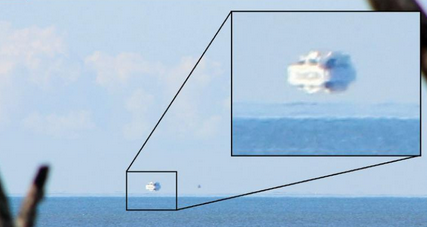
\includegraphics[scale=1]{Images/Mirage.PNG}
\end{center}
\begin{center}
     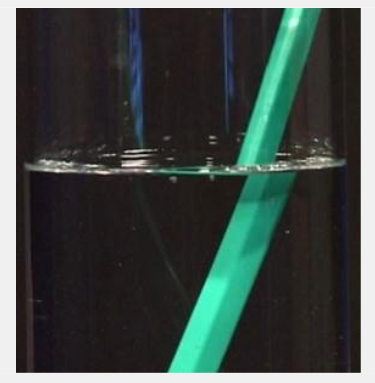
\includegraphics[scale=1]{Images/Crayon_brise.PNG}
\end{center}
Un crayon posé dans un verre d'eau semble se briser lors de son passage dans le verre ...
\end{multicols}
\textbf{Cela est dû au changement du milieu de propagation de la lumière !}
%    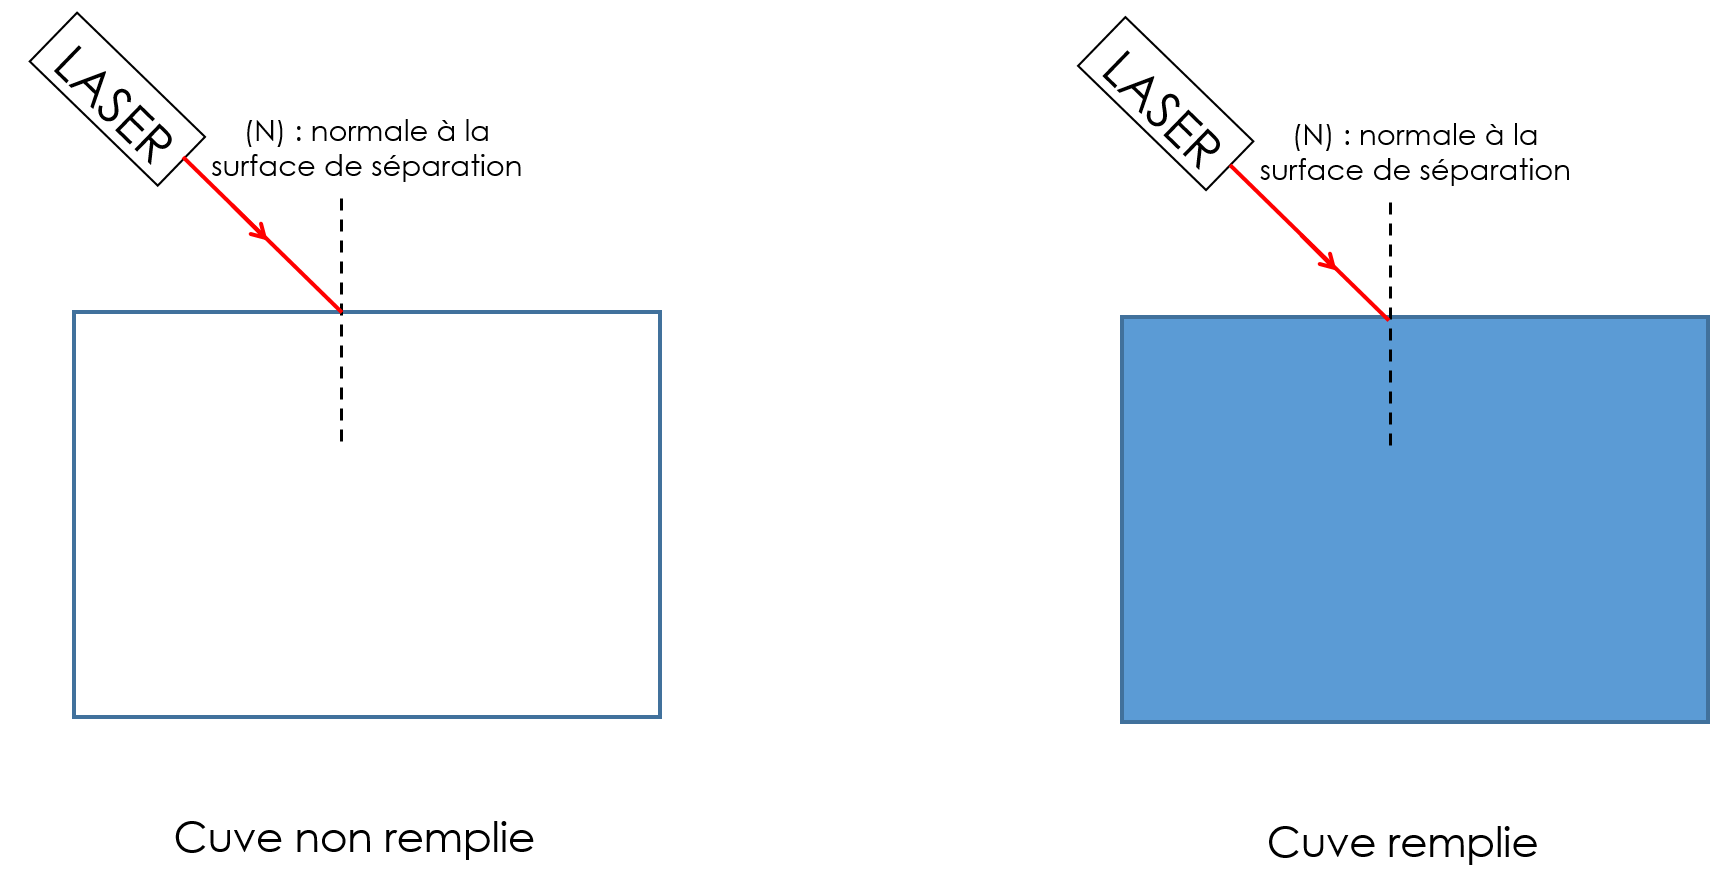
\includegraphics[scale=0.5]{Images/TP/TP9/Experience_intro.png}
%\end{center}
%\begin{wrapfigure}{r}{0.3\textwidth}
%\vspace{-0cm}
%    \centering
%     \includegraphics[width=0.32\textwidth]{Images/Cours/Chapitre_3/Haut_parleur_bougie.PNG}
%   \end{wrapfigure}
%\textcolor{green}{\underline{Expérience 1 :}} On place un laser face à une cuve vide. On vaporise de l'eau sur le trajet de la lumière. Observations : \\
%\textcolor{red}{En vaporisant de l'eau sur le parcours de la lumière, on observe que \underline{la lumière se propage en ligne droite}.}\\
%\textcolor{green}{\underline{Expérience 2 :}} Cette fois, on remplit la cuve d'un mélange eau-fluoréscine qui permet de visualiser le trajet de la lumière. Observations : \\
%\textbf{Observations :} \textcolor{red}{Par rapport à l'expérience 1, on remarque que la lumière du laser n'arrive pas au même endroit sur l'écran. Elle a été \underline{déviée}.}

\subsection{Représentation de la situation}
\begin{center}
    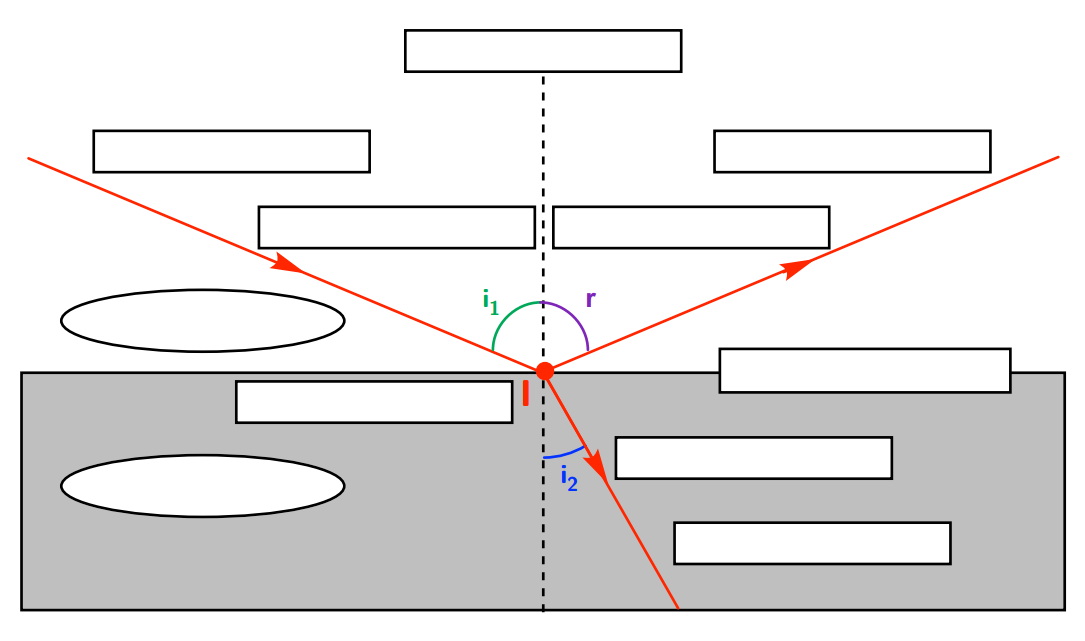
\includegraphics[scale=0.7]{Images/Schema_changement_milieu.PNG}
\end{center}

\subsection{Les lois de Snell-Descartes}
\subsubsection{Loi sur la réflexion}
\begin{tcolorbox}[colback=red!5!white,colframe=red!75!black,title=\textbf{1$^{\text{ère}}$ loi de Snell-Descartes :}, upperbox=invisible]
Le rayon incident et le rayon réfléchi appartiennent au même plan appelé \textcolor{red}{plan d'incidence}.\\
L'angle d'incidence $i_1$ et l'angle de réflexion $r$ sont égaux :
\begin{empheq}[box=\fbox]{equation*}
    i_1=r
\end{empheq}
\end{tcolorbox}

\subsubsection{Loi sur la réfraction}
Lors du passage du milieu d'incidence au milieu de réfraction, la lumière est déviée : c'est le phénomène de \textcolor{red}{réfraction}.
\begin{tcolorbox}[colback=red!5!white,colframe=red!75!black,title=\textbf{2$^{\text{ème}}$ loi de Snell-Descartes :}, upperbox=invisible]
Le rayon incident, réfracté appartiennent au même plan appelé \textcolor{red}{plan d'incidence}.\\
L'angle d'incidence $i_1$ et l'angle de réfraction $i_2$ sont reliés par la formule suivante :
\begin{empheq}[box=\fbox]{equation*}
    n_1 \sin\left(i_1\right)= n_2 \sin\left(i_2\right)
\end{empheq}
\end{tcolorbox}

\begin{center}
    \begin{tabular}{|c|C{0.15}|C{0.13}|C{0.15}|C{0.17}|C{0.15}|}
        \hline
        \cellcolor{blue!25}Milieu & vide & air & eau & plexiglas (TP 9) & diamant \\
        \hline
         \cellcolor{blue!25}Indice optique n & 1 (exactement) & 1,00 & 1,33 &  & 2,52 \\
         \hline
    \end{tabular}
\end{center}
\begin{Large}
    \ding{45}
\end{Large}\textbf{Exercice 9, 10, 11, 12, 22, 29, 31}

\subsection{Dispersion de la lumière}
\begin{Large}
    \ding{43}
\end{Large}
Voir \textit{TP 10 : L'apparition d'un arc-en-ciel}.
\begin{multicols}{2}
    \begin{center}
        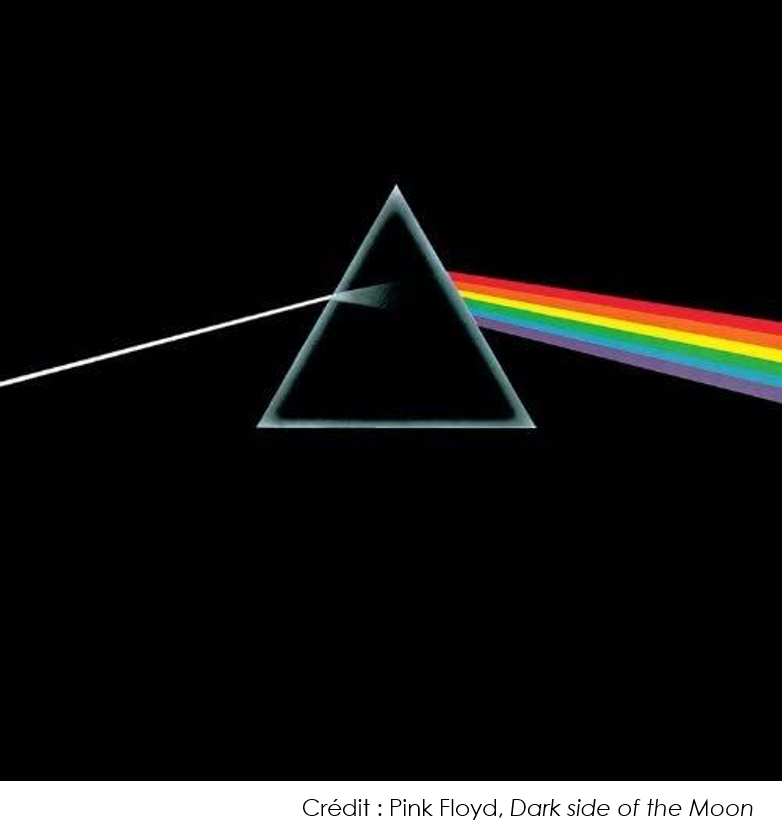
\includegraphics[scale=0.5]{Images/Pink_floyd.png}
    \end{center}
    
    \begin{tcolorbox}[colback=green!5!white,colframe=green!75!black,title=\textbf{Milieu dispersif et spectre:}, upperbox=invisible]
Un milieu est dit \textcolor{red}{disersif} si son indice optique $n$ dépend de la longueur d'onde (c'est-à-dire de la couleur) de la lumière qui le traverse.\\

L'image de cette décomposition des couleurs sur un écran est appelé le \textcolor{red}{spectre de la lumière blanche}.
\end{tcolorbox}
\end{multicols}

\begin{tcolorbox}[colback=green!5!white,colframe=green!75!black,title=\textbf{Source monochromatique ou polychromatique:}]
Une source de lumière est dite \textcolor{red}{monochromatique} si elle produit une lumière composée d'une seule longueur d'onde. Par exemple : un laser.\\

Une source de lumière est dite \textcolor{red}{polychromatique} si elle produit une lumière composée de plusieurs longueurs d'ondes. Par exemple : le soleil.
\end{tcolorbox}

\begin{Large}
    \ding{45}
\end{Large}\textbf{Exercice 14, 19}
\section{Modélisation de l'\oe il par une lentille}
\begin{Large}
    \ding{43}
\end{Large}
Voir \textit{Activité : L'\oe il, un instrument remarquable}.

\subsection{Modélisation}
Tout comme une lentille, l'\oe il permet de visualiser un \textcolor{red}{objet} à une certaine distance en faisant converger les rayons lumineux issus de cet objet pour en produire une \textcolor{red}{image} sur la rétine :
\begin{center}
    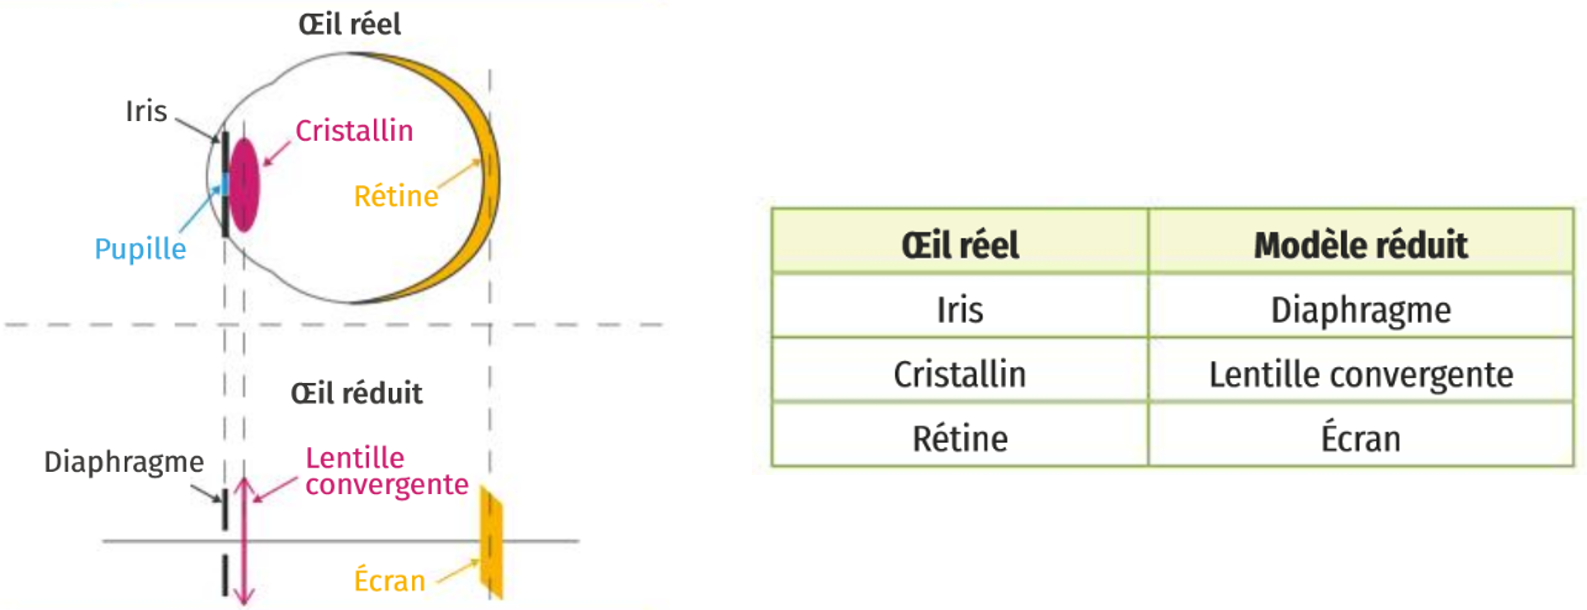
\includegraphics[scale=0.5]{Images/Modele_oeil.PNG}
\end{center}

\subsection{Détermination graphique d'une image par une lentille convergente}

\begin{tcolorbox}[colback=green!5!white,colframe=green!75!black,title=\textbf{Lentille convergente :}]
\begin{multicols}{2}
    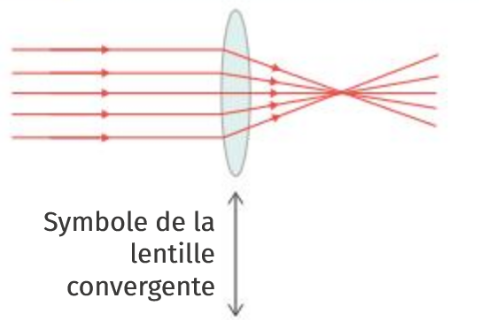
\includegraphics[scale=0.7]{Images/Lentille.PNG}
    
    %Une lentille est caractérisée par son \textcolor{red}{centre optique} O par lequel passe l'axe optique $\Delta$, son \textcolor{red}{foyer image} F' et \textcolor{red}{son foyer objet} F.
\end{multicols}
\end{tcolorbox}

\begin{tcolorbox}[colback=red!5!white,colframe=red!75!black,title=\textbf{Construction d'une image par une lentille :}]
\begin{itemize}
    \item Le rayon passant par le centre optique O \textbf{n'est pas dévié} ;
    \item Les rayons arrivant parallèlement à l'axe optique $\Delta$ \textbf{ressortent sur le foyer image F'} ;
    \item Les rayons passant par le foyer objet F \textbf{ressortent parallèle à l'axe optique $\Delta$}.
\end{itemize}
\end{tcolorbox}

\begin{center}
    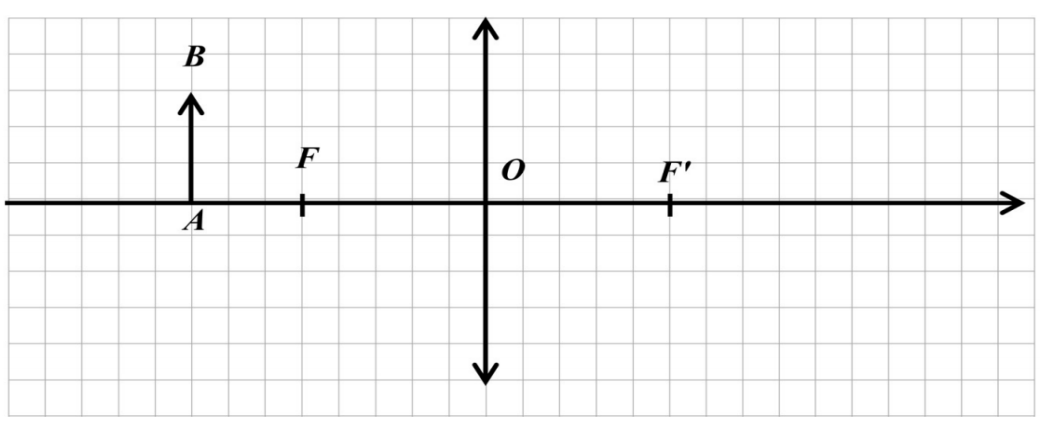
\includegraphics[scale=1]{Images/Lentille_construction_eleve.PNG}
\end{center}

\subsection{Grandissement}
Pour un objet de taille AB, on obtient une image A'B'. \begin{tcolorbox}[colback=green!5!white,colframe=green!75!black,title=\textbf{Grandissement :}, upperbox=invisible]
On définit le \textcolor{red}{grandissement} $\gamma$ d'une lentille comme le rapport entre la \textcolor{red}{hauteur algébrique} de l'image $\overline{\text{A'B'}}$ sur la \textcolor{red}{hauteur algébrique} de l'objet $\overline{\text{AB}}$ :
\begin{empheq}[box=\fbox]{equation*}
    \gamma = \frac{\overline{A'B'}}{\overline{AB}}
\end{empheq}
\begin{itemize}
    \item Si $\gamma$ est négatif, alors l'image est renversée ;
    \item Si $\abs{\gamma}$ est plus petit que 1, alors l'image est rétrécie.
\end{itemize}
\end{tcolorbox}

\begin{mdframed}[style=autreexo]
\textbf{\bsc{Exercice de cours} - Grandissement}\\
Sur la construction précédente, déterminer $\gamma$.
\end{mdframed}

\begin{Large}
    \ding{45}
\end{Large}\textbf{Exercice 25, Appareil photo}
  %\modeCorrection

\renewcommand{\thesubsection}{\textcolor{red}{\Roman{section}.\arabic{subsection}}}
\renewcommand{\thesubsubsection}{\textcolor{red}{\Roman{section}.\arabic{subsection}.\alph{subsubsection}}}

\setcounter{section}{0}
\sndEnTeteCoursQuatre

\begin{mdframed}[style=titr, leftmargin=60pt, rightmargin=60pt, innertopmargin=7pt, innerbottommargin=7pt, innerrightmargin=8pt, innerleftmargin=8pt]

\begin{center}
\large{\textbf{Chapitre 4 : Propagation de la lumière dans les milieux}}
\end{center}
\end{mdframed}
La lumière se propage-t'elle toujours en ligne droite ? Quelles sont les lois qui gouvernent la propagation de la lumière ?

\begin{tcolorbox}[colback=blue!5!white,colframe=blue!75!black,title=Mots clés du chapitre :]
Lois de Snell-Descartes, réfraction, réflexion, dispersion, lentille convergent, image, objet, modélisation de l'\oe il.
\end{tcolorbox}


\section{Propagation de la lumière dans un milieu homogène}
\subsection{Généralités}
\begin{tcolorbox}[colback=red!5!white,colframe=red!75!black,title=\textbf{Propriété de la propagation :}]
La lumière se propage de façon \textcolor{red}{rectiligne} (en ligne droite) dans un milieu \textcolor{red}{transparent} (qui laisse passer la lumière) et \textcolor{red}{homogène} (dont les propriétés ne changent pas dans l'espace).
\end{tcolorbox}

\subsection{Vitesse de la lumière}
La vitesse, aussi appelée \textcolor{red}{célérité} de la lumière, est c = 299 792 458~m$\cdot$s$^{-1}$. Aucun objet matériel ne peut aller plus vite que la lumière.
\begin{tcolorbox}[colback=red!5!white,colframe=red!75!black,title=\textbf{Propriété de la vitesse de la lumière :}]
On retiendra que dans le vide et dans l'air :
\begin{empheq}[box=\fbox]{equation*}
    c_{vide}\simeq c_{air}=3\times10^8~\text{m$\cdot$s$^{-1}$}
\end{empheq}
\end{tcolorbox}

\begin{tcolorbox}
[colback=green!5!white,colframe=green!75!black,title=\textbf{Indice optique d'un milieu homogène :}]
Un milieu transparent et homogène est caractérisé par son \textcolor{red}{indice optique} (ou \textcolor{red}{indice de réfraction}), noté $n$ défini par :
\begin{equation*}
    n_{\text{milieu}} = \frac{c}{v_{\text{milieu}}}
\end{equation*}
avec :
\begin{itemize}
    \item c la célérité de la lumière dans le vide, 
    \item $v_{\text{milieu}}$ la vitesse de la lumière dans le milieu.
\end{itemize}
\importantbox{L'indice optique d'un milieu est toujours supérieur à 1 : $n_{milieu}>1$.}
\end{tcolorbox}

\section{Changement du milieu de propagation : lois de Snell-Descartes}
\begin{Large}
    \ding{43}
\end{Large}
Voir TP 9 : Les lois de la réfraction et de la réflexion.
\subsection{Mise en évidence expérimentale}
\begin{multicols}{2}
Avez-vous déjà observé un bateau qui semble flotter dans les airs ? C'est le phénomène de \textit{Fata Morgana} qui peut être observé au-dessus d'une étendue d'eau qui reste froide par rapport à l'air.
\begin{center}
     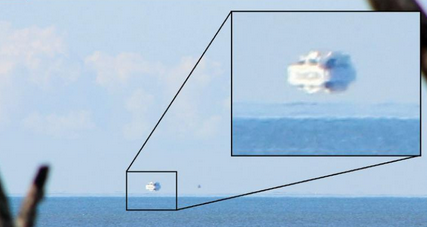
\includegraphics[scale=1]{Images/Mirage.PNG}
\end{center}
\begin{center}
     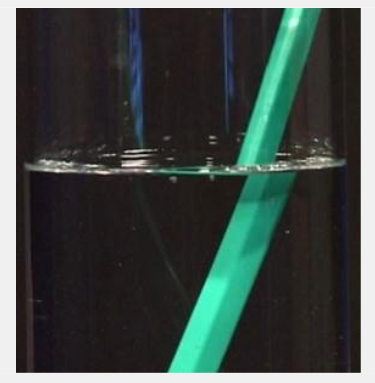
\includegraphics[scale=1]{Images/Crayon_brise.PNG}
\end{center}
Un crayon posé dans un verre d'eau semble se briser lors de son passage dans le verre ...
\end{multicols}
\textbf{Cela est dû au changement du milieu de propagation de la lumière !}
%    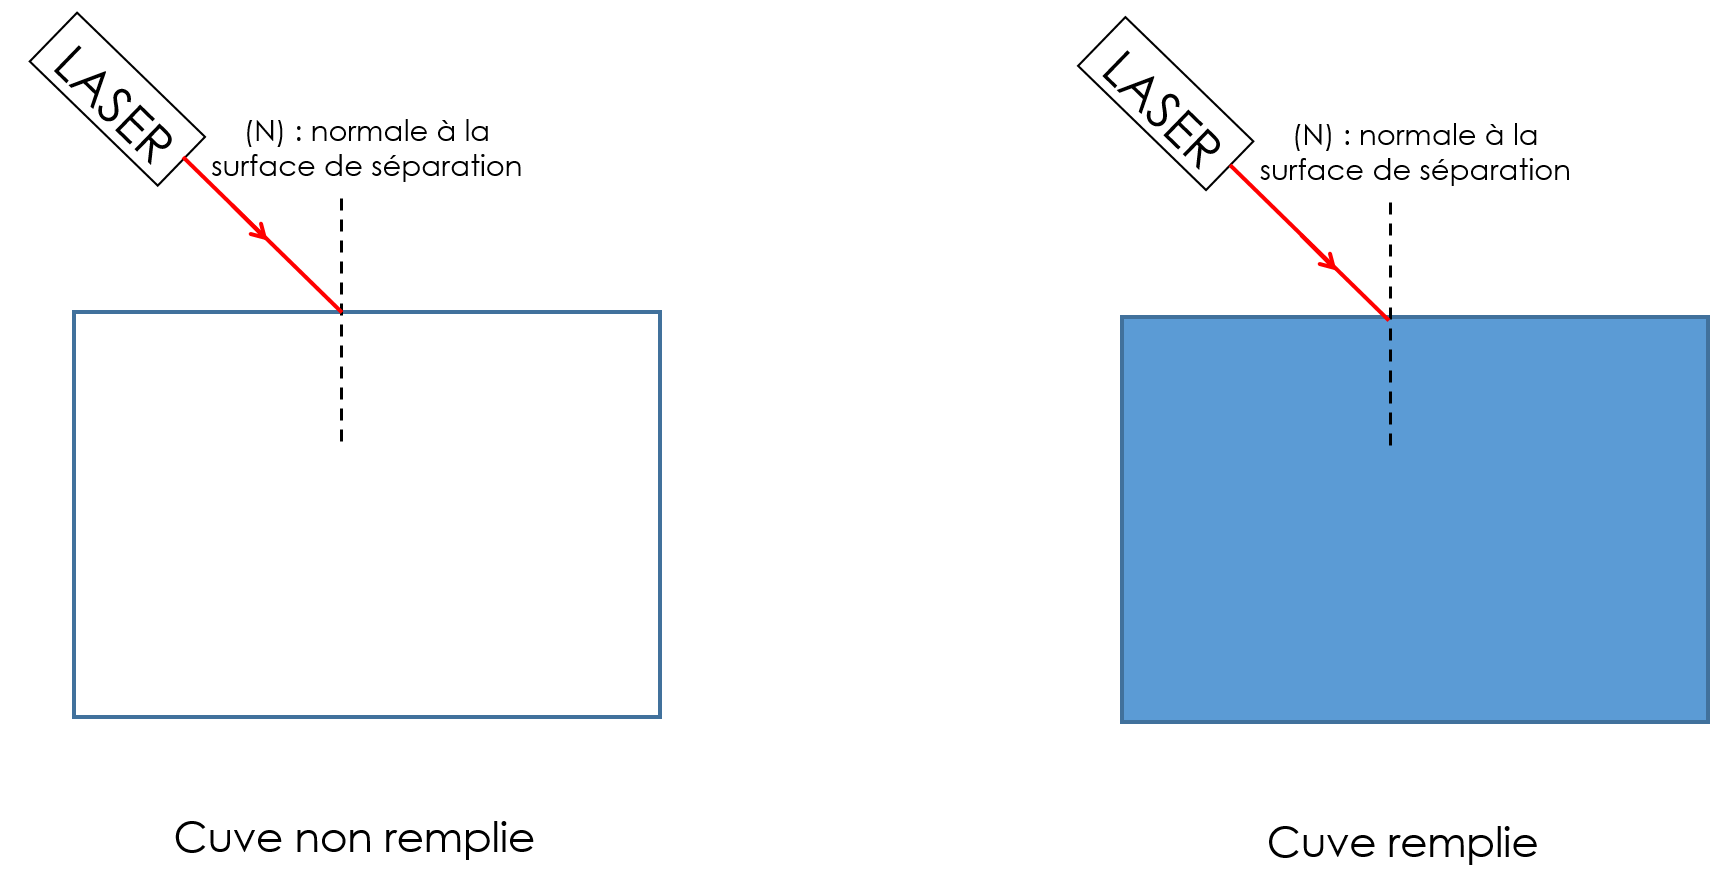
\includegraphics[scale=0.5]{Images/TP/TP9/Experience_intro.png}
%\end{center}
%\begin{wrapfigure}{r}{0.3\textwidth}
%\vspace{-0cm}
%    \centering
%     \includegraphics[width=0.32\textwidth]{Images/Cours/Chapitre_3/Haut_parleur_bougie.PNG}
%   \end{wrapfigure}
%\textcolor{green}{\underline{Expérience 1 :}} On place un laser face à une cuve vide. On vaporise de l'eau sur le trajet de la lumière. Observations : \\
%\textcolor{red}{En vaporisant de l'eau sur le parcours de la lumière, on observe que \underline{la lumière se propage en ligne droite}.}\\
%\textcolor{green}{\underline{Expérience 2 :}} Cette fois, on remplit la cuve d'un mélange eau-fluoréscine qui permet de visualiser le trajet de la lumière. Observations : \\
%\textbf{Observations :} \textcolor{red}{Par rapport à l'expérience 1, on remarque que la lumière du laser n'arrive pas au même endroit sur l'écran. Elle a été \underline{déviée}.}

\subsection{Représentation de la situation}
\begin{center}
    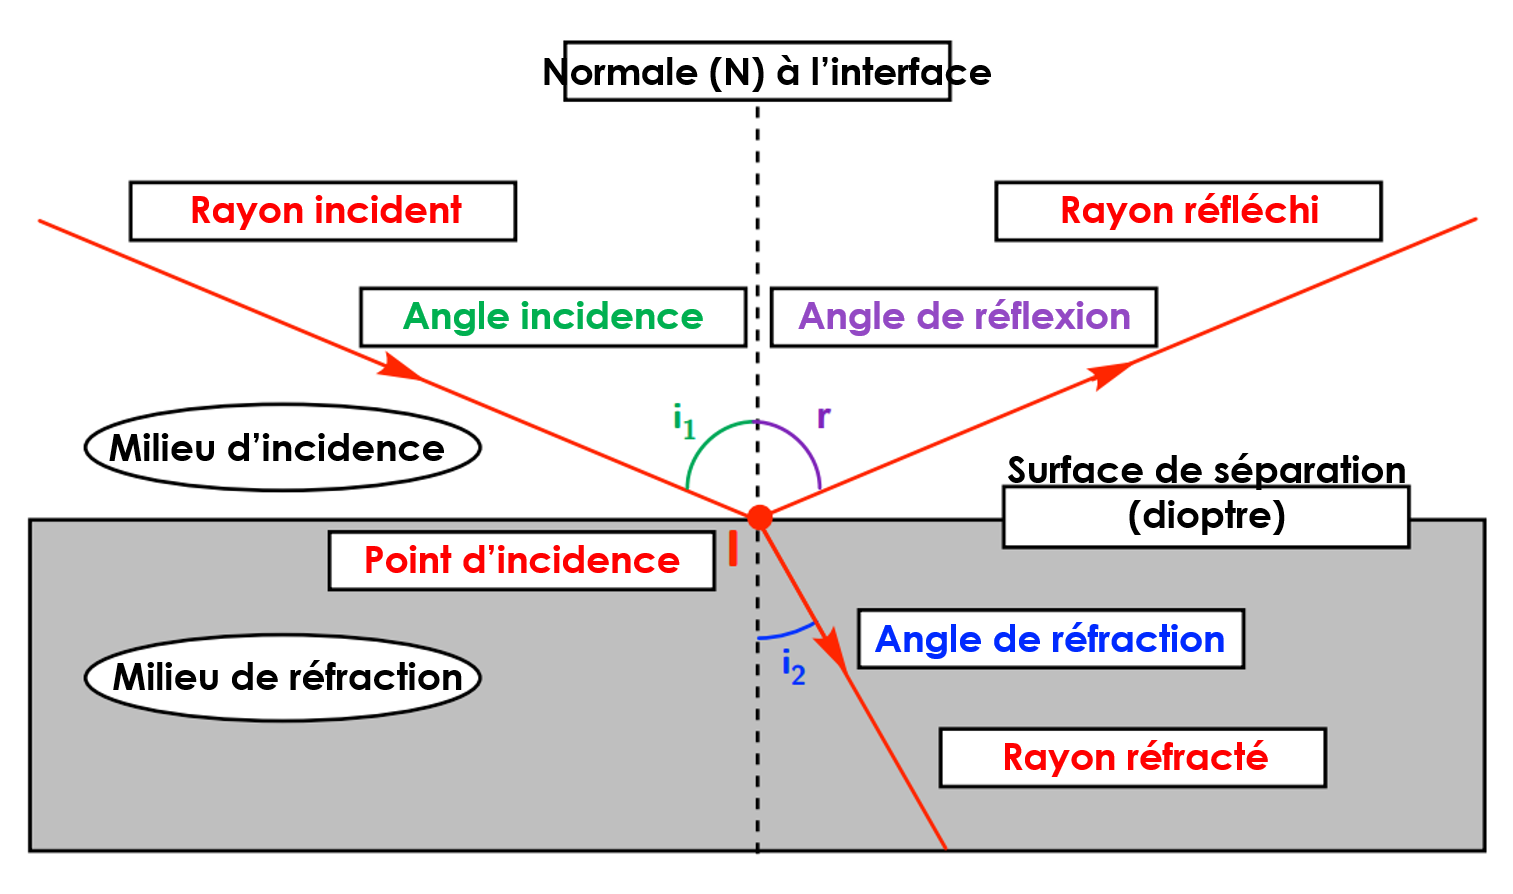
\includegraphics[scale=0.6]{Images/Schema_changement_milieu_corrige.png}
\end{center}

\subsection{Les lois de Snell-Descartes}
\subsubsection{Loi sur la réflexion}
\begin{tcolorbox}[colback=red!5!white,colframe=red!75!black,title=\textbf{1$^{\text{ère}}$ loi de Snell-Descartes :}]
Le rayon incident et le rayon réfléchi appartiennent au même plan appelé \textcolor{red}{plan d'incidence}.\\
L'angle d'incidence $i_1$ et l'angle de réflexion $r$ sont égaux :
\begin{empheq}[box=\fbox]{equation*}
    i_1=r
\end{empheq}
\end{tcolorbox}

\subsubsection{Loi sur la réfraction}
Lors du passage du milieu d'incidence au milieu de réfraction, la lumière est déviée : c'est le phénomène de \textcolor{red}{réfraction}.
\begin{tcolorbox}[colback=red!5!white,colframe=red!75!black,title=\textbf{2$^{\text{ème}}$ loi de Snell-Descartes :}]
Le rayon incident, réfracté appartiennent au même plan appelé \textcolor{red}{plan d'incidence}.\\
L'angle d'incidence $i_1$ et l'angle de réfraction $i_2$ sont reliés par la formule suivante :
\begin{empheq}[box=\fbox]{equation*}
    n_1 \sin\left(i_1\right)= n_2 \sin\left(i_2\right)
\end{empheq}
\end{tcolorbox}

\begin{center}
    \begin{tabular}{|c|C{0.15}|C{0.13}|C{0.15}|C{0.17}|C{0.15}|}
        \hline
        \cellcolor{blue!25}Milieu & vide & air & eau & plexiglas (TP 9) & diamant \\
        \hline
         \cellcolor{blue!25}Indice optique n & 1 (exactement) & 1,00 & 1,33 & 1,48 & 2,52 \\
         \hline
    \end{tabular}
\end{center}
\begin{Large}
    \ding{45}
\end{Large}\textbf{Exercice 9, 10, 11, 12, 22, 29, 31}

\subsection{Dispersion de la lumière}
\begin{Large}
    \ding{43}
\end{Large}
Voir TP 10 : L'apparition d'un arc-en-ciel.
\begin{multicols}{2}
    \begin{center}
        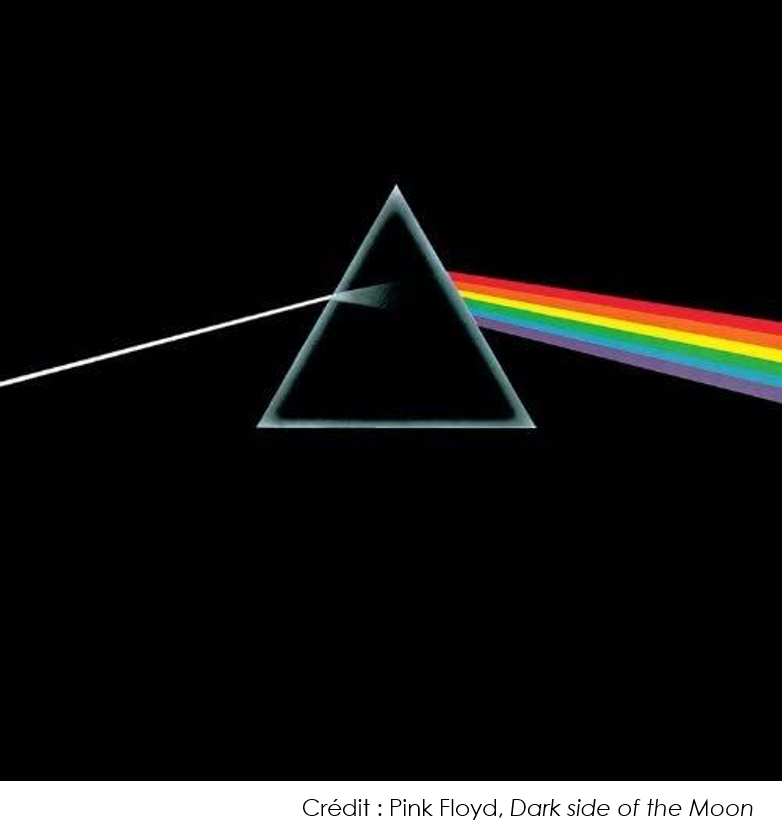
\includegraphics[scale=0.5]{Images/Pink_floyd.png}
    \end{center}
    
    \begin{tcolorbox}[colback=green!5!white,colframe=green!75!black,title=\textbf{Milieu dispersif et spectre:}]
Un milieu est dit \textcolor{red}{dispersif} si son indice optique $n$ dépend de la longueur d'onde (c'est-à-dire de la couleur) de la lumière qui le traverse.\\

L'image de cette décomposition des couleurs sur un écran est appelé le \textcolor{red}{spectre d'émission} de la source (ci-contre le spectre d'émission de la lumière blanche).
\end{tcolorbox}
\end{multicols}

\begin{tcolorbox}[colback=green!5!white,colframe=green!75!black,title=\textbf{Source monochromatique ou polychromatique:}]
Une source de lumière est dite \textcolor{red}{monochromatique} si elle produit une lumière composée d'une seule longueur d'onde. Par exemple : un laser.\\

Une source de lumière est dite \textcolor{red}{polychromatique} si elle produit une lumière composée de plusieurs longueurs d'ondes. Par exemple : le soleil.
\end{tcolorbox}

\begin{Large}
    \ding{45}
\end{Large}\textbf{Exercice 14, 19}
\section{Modélisation de l'\oe il par une lentille}
\begin{Large}
    \ding{43}
\end{Large}
Voir Activité : L'\oe il, un instrument remarquable.

\subsection{Modélisation}
Tout comme une lentille, l'\oe il permet de visualiser un \textcolor{red}{objet} à une certaine distance en faisant converger les rayons lumineux issus de cet objet pour en produire une \textcolor{red}{image} sur la rétine :
\begin{center}
    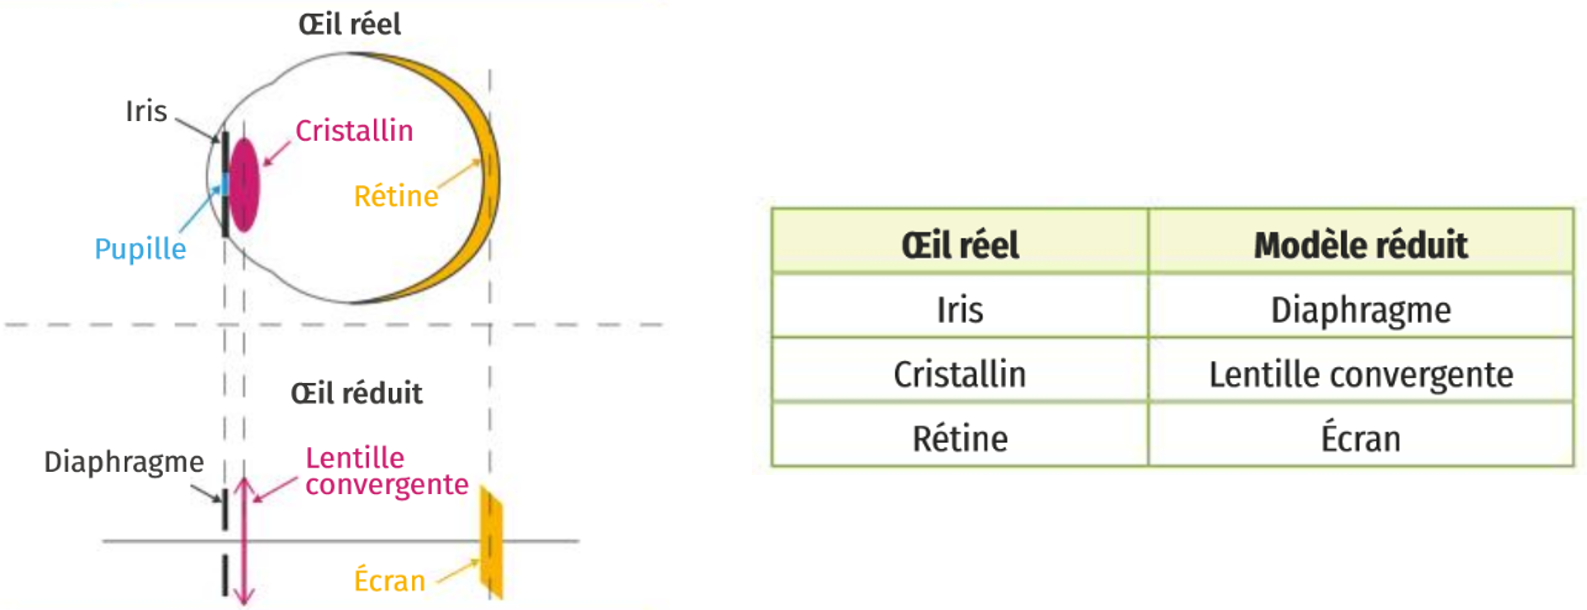
\includegraphics[scale=0.5]{Images/Modele_oeil.PNG}
\end{center}

\subsection{Détermination graphique d'une image par une lentille convergente}

\begin{tcolorbox}[colback=green!5!white,colframe=green!75!black,title=\textbf{Lentille convergente :}]
\begin{multicols}{2}
    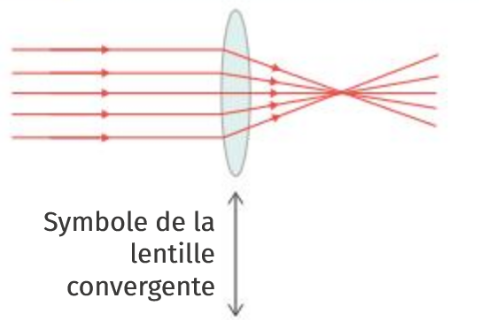
\includegraphics[scale=0.7]{Images/Lentille.PNG}
    
    Une lentille est caractérisée par son \textcolor{red}{centre optique} O par lequel passe l'axe optique $\Delta$, son \textcolor{red}{foyer image} F' et \textcolor{red}{son foyer objet} F.
\end{multicols}
\end{tcolorbox}
%\newpage

%\begin{center}
 %   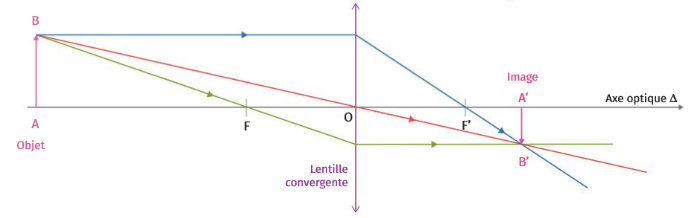
\includegraphics[scale=1]{Images/Lentille_construction.png}
%\end{center}

\begin{tcolorbox}[colback=red!5!white,colframe=red!75!black,title=\textbf{Construction d'une image par une lentille :}]
\begin{itemize}
    \item Le rayon passant par le centre optique O \textbf{n'est pas dévié} ;
    \item Les rayons arrivant parallèlement à l'axe optique $\Delta$ \textbf{ressortent sur le foyer image F'} ;
    \item Les rayons passant par le foyer objet F \textbf{ressortent parallèle à l'axe optique $\Delta$}.
\end{itemize}
\end{tcolorbox}

\begin{center}
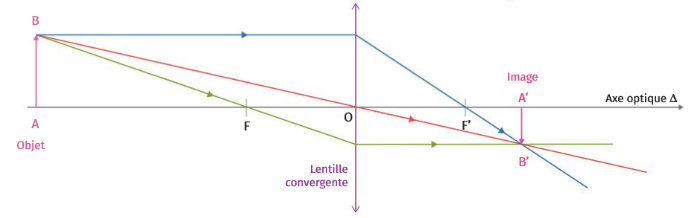
\includegraphics[scale=1]{Images/Lentille_construction.png}
\end{center}

\subsection{Grandissement}
Pour un objet de taille AB, on obtient une image A'B'. 
\begin{tcolorbox}[colback=green!5!white,colframe=green!75!black,title=\textbf{Grandissement :}]
On définit le \textcolor{red}{grandissement} $\gamma$ d'une lentille comme le rapport entre la \textcolor{red}{hauteur algébrique} de l'image $\overline{\text{A'B'}}$ sur la \textcolor{red}{hauteur algébrique} de l'objet $\overline{\text{AB}}$ :
\begin{empheq}[box=\fbox]{equation*}
    \gamma = \frac{\overline{A'B'}}{\overline{AB}}
\end{empheq}
\begin{itemize}
    \item Si $\gamma$ est négatif, alors l'image est renversée ;
    \item Si $\abs{\gamma}$ est plus petit que 1, alors l'image est plus petite que l'objet.
\end{itemize}
\end{tcolorbox}

\begin{mdframed}[style=autreexo]
\textbf{\bsc{Exercice de cours} - Grandissement}\\
Sur la construction précédente, déterminer $\gamma$.
\end{mdframed}

\begin{Large}
    \ding{45}
\end{Large}\textbf{Exercice 25, Appareil photo}

  %%%%%%%%%% Exercices %%%%%%%%
  
  %%%%%%%%%% Activités %%%%%%%%

 
  %%%%%%%%%% TP %%%%%%%%%%%%%%%
  %\modeCorrection

%%%% début de la page
\renewcommand{\thesection}{\textcolor{red}{Partie \Roman{section} -}}
\renewcommand{\thesubsection}{\textcolor{red}{\Roman{section}.\arabic{subsection}}}
\renewcommand{\thesubsubsection}{\textcolor{red}{\Roman{section}.\arabic{subsection}.\alph{subsubsection}}}

\setcounter{section}{0}
\setcounter{document}{0}
\sndEnTeteTPNeuf

\begin{center}
\begin{mdframed}[style=titr, leftmargin=60pt, rightmargin=60pt, innertopmargin=7pt, innerbottommargin=7pt, innerrightmargin=8pt, innerleftmargin=8pt]

\begin{center}
\large{\textbf{TP 9 : Phénomènes de réflexion en réfraction de la lumière
}}
\end{center}
\end{mdframed}
\end{center}

%\begin{tableauCompetences}
%    APP & Exploiter des explications orales pour rédiger un protocole & & & & \\
 %   \hline
  %  REA & Réaliser une série de mesures ; relever les résultats obtenus & & & & \\
   %  \hline 
    % REA & Utiliser une grandeur quotient pour déterminer le numérateur ou le dénominateur& & & & \\
     %\hline 
   % COM & Rendre compte de façon écrite & & & & \\
    %\hline
    %VAL & Analyser l’ensemble des résultats de façon critique  & & & &
%\end{tableauCompetences}


%%%% objectifs
\begin{tcolorbox}[colback=blue!5!white,colframe=blue!75!black,title=Objectifs de la séance :]
\begin{itemize}
    \item Mettre en évidence les phénomène de réflexion et de réfraction de la lumière ;
    \item Identifier une relation de proportionnalité ;
    \item Valider une loi en réalisant une série de mesures 
    \item Déterminer l'indice de réfraction d'un milieu ;
\end{itemize}
\end{tcolorbox}

%%%% Consignes
\begin{tcolorbox}[colback=red!5!white,colframe=red!75!black,title= Consignes :]
\begin{itemize}
    \item Faire attention au matériel lors de son utilisation ;
\end{itemize}
\end{tcolorbox}

%%%% contexte
\section{Mise en évidence expérimentale}
\begin{tcolorbox}[colback=orange!5!white,colframe=orange!75!black,title= Expérience introductive :]
Réalisons l'expérience suivante : on éclaire par une lumière laser une cuve initialement vide. Puis on remplit la cuve d'un mélange d'eau et d'une substance fluorescente permettant de visualiser la lumière laser. Voici les schémas de l'expérience avant et après remplissage de la cuve :
\begin{center}
    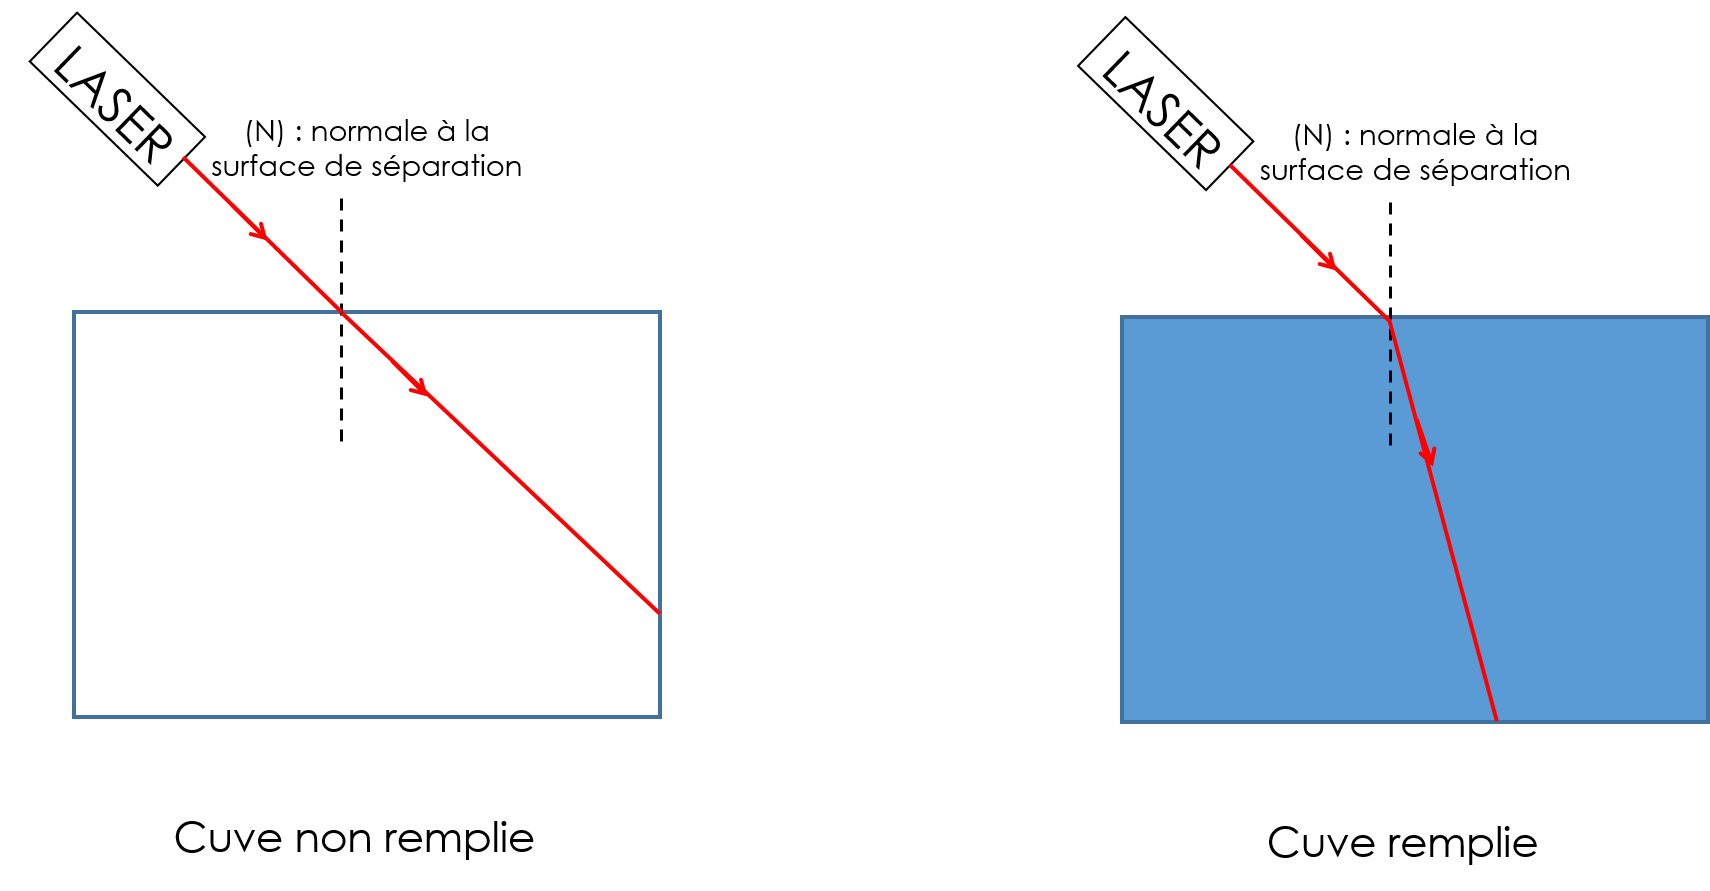
\includegraphics[scale=0.4]{Images/Experience_intro_correc.png}
\end{center}
\textbf{\underline{Observations :}}
\texteTrouMultiLignes{Lorsque la cuve est vide, la lumière provenant du laser se propage en ligne droite dans la cuve. En revanche, lorsque la cuve est remplie du mélange eau-fluorescéine, la lumière est déviée lors du passage air-mélange. La lumière se rapproche de la normale à l'interface.}{4}

\problematique{Peut-on relier les rayons refracté et réfléchi au rayon incident ? Peut-on mesurer un indice de réfraction d'un milieu ?}
\end{tcolorbox}


\begin{mdframed}[style=autreexo]
\textbf{\bsc{Liste du matériel}}
\begin{itemize}
    \item Une source de lumière collimatée avec son alimentation électrique ;
    \item Un demi-cylindre de plexiglas sur un disque gradué pivotant ;
    \item un ordinateur muni du logiciel tableau-grapheur ;
\end{itemize}
\end{mdframed}

%%%% documents

%%%%
\section{Lois de Snell-Descartes}
\begin{doc}{Quelques mots de vocabulaire}
\begin{center}
\vspace{-0.5cm}
     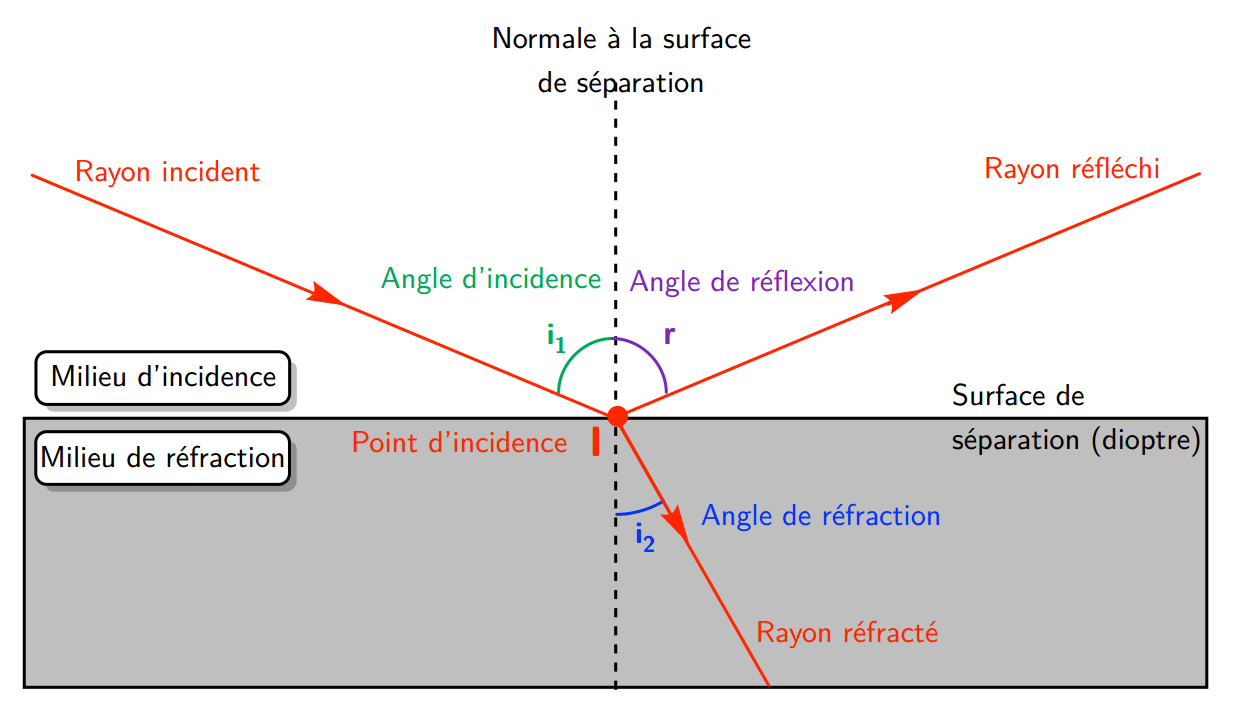
\includegraphics[scale=0.5]{Images/Figure_propagation.PNG}
\end{center}
\importantbox{Les angles d'incidence $i_1$, de reflexion $r$ et de réfraction $i_2$ sont toujours comptés à partir de la normale à la surface de séparation.}
\end{doc}

\subsection{Loi de Snell-Descartes pour la réflexion}
\begin{multicols}{2}
\question{Allumer la lampe et régler le zéro du disque gradué à l'aide des vis de réglage.}{Fais en classe.}{0}
\\
\question{Pour chaque valeur d'angle d'incidence $i_1$, mesurer l'angle de réflexion $r$ et compléter le tableau suivant :}{\begin{center}
    \begin{tabular}{|c|C{0.06}|C{0.06}|C{0.06}|C{0.06}|C{0.06}|C{0.06}|C{0.06}|C{0.06}|C{0.06}|}
        \hline
        $i_1$ (en $\degree$) & 0 & 5 & 10 & 15 & 20 & 30 & 35 & 40 & 45 \\
        \hline
        $r$ (en $\degree$) & 5 & 10 & 15 & 20 & 25 & 30 & 35 & 40 & 45\\
        \hline
    \end{tabular}
\end{center}}{0}
\begin{center}
    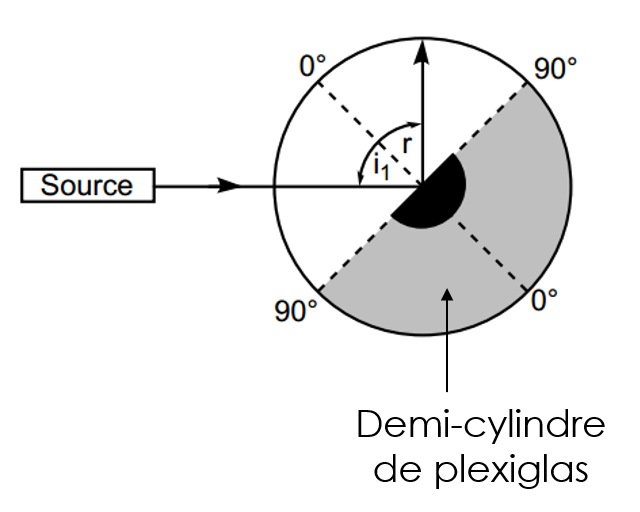
\includegraphics[width=0.4\textwidth]{Images/Schema_exp.PNG}
\end{center}
\end{multicols}

\begin{center}
    \begin{tabular}{|c|C{0.06}|C{0.06}|C{0.06}|C{0.06}|C{0.06}|C{0.06}|C{0.06}|C{0.06}|C{0.06}|}
        \hline
        $i_1$ (en $\degree$) & 0 & 5 & 10 & 15 & 20 & 30 & 35 & 40 & 45 \\
        \hline
        $r$ (en $\degree$) & & & & & & & & &\\
        \hline
    \end{tabular}
\end{center}
%\\
\begin{tcolorbox}[colback=red!5!white,colframe=red!75!black,title=\textbf{Loi de Snell-Descartes pour la réflexion : }]
\texteTrouMultiLignes{Les rayons incident et réfléchis sont tels que les angles d'incidence $i_1$ et de réflexion $r$ sont égaux : 
\begin{empheq}[box=\fbox]{equation*}
    i_1=r
\end{empheq}.}{2}
\end{tcolorbox}

\subsection{Loi de Snell-Descartes pour la réfraction}
\begin{center}
    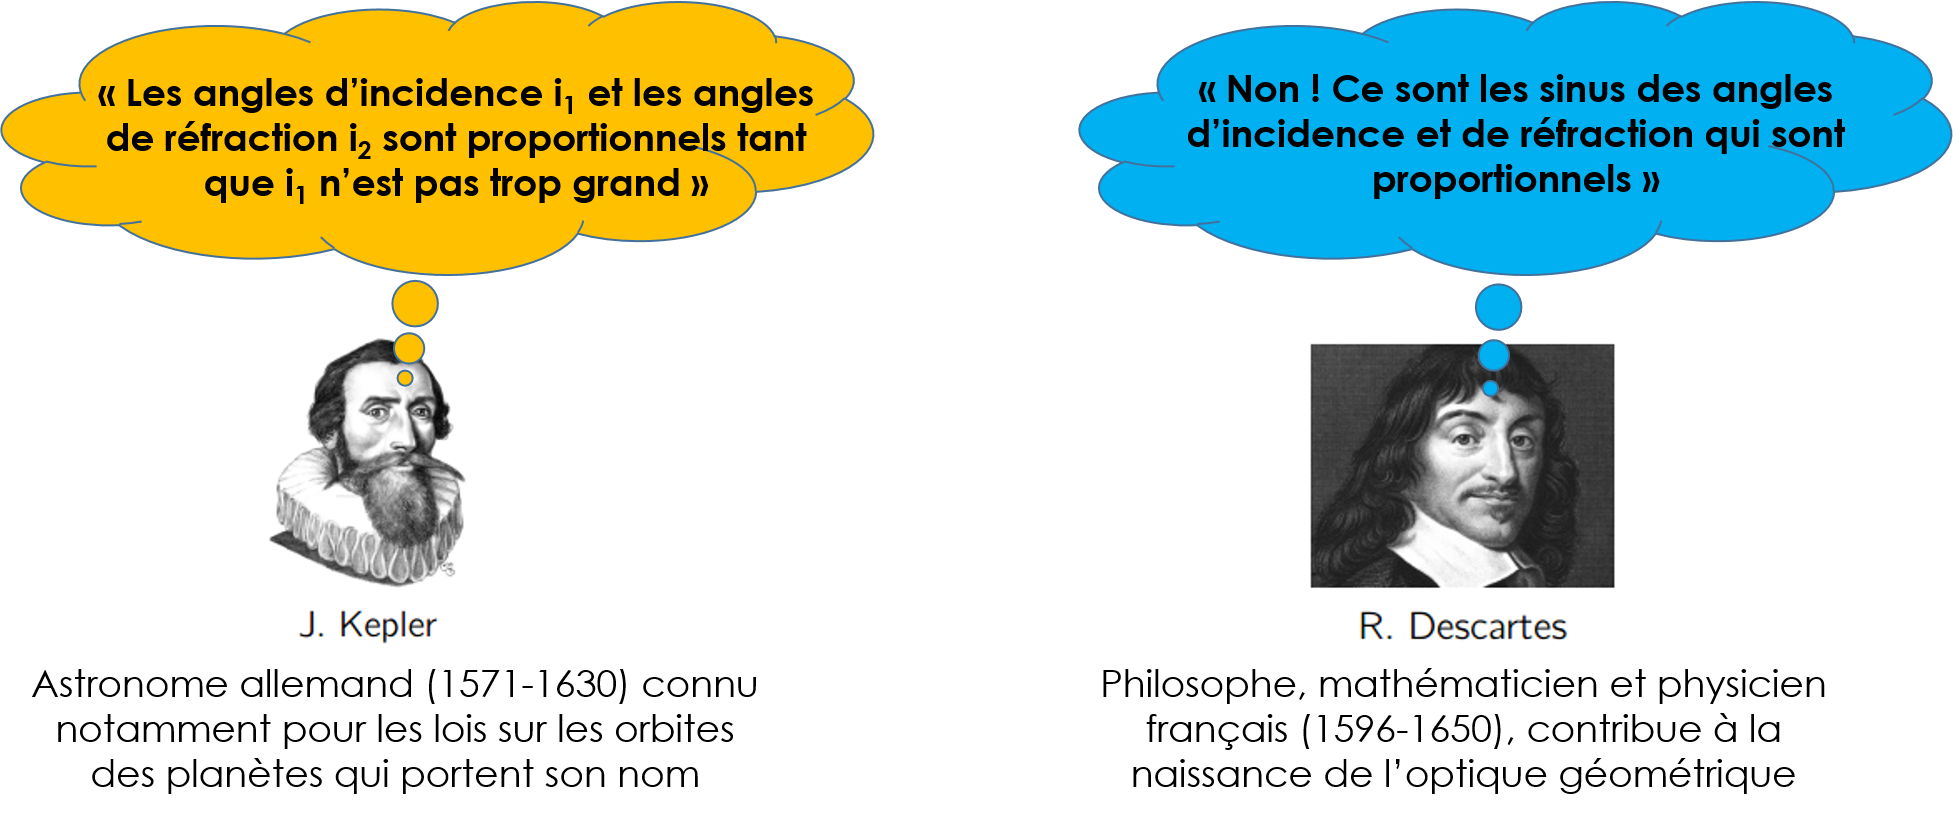
\includegraphics[scale=0.5]{Images/DescartesvsKepler.png}
\end{center}

\problematique{Lequel de ces deux scientifiques avait raison ?}
\subsubsection{Expérience}

\begin{multicols}{2}
\question{Allumer la lampe et régler le zéro du disque gradué sur le chemin du faisceau lumineux.}{Réalisé en classe.}{0}
\\
\question{Pour chaque valeur d'angle d'incidence $i_1$, mesurer l'angle de réfraction $i_2$ et compléter le tableau suivant (on ne prendra que 2 chiffres après la virgule pour le sinus) :}{~}{0}
\begin{center}
    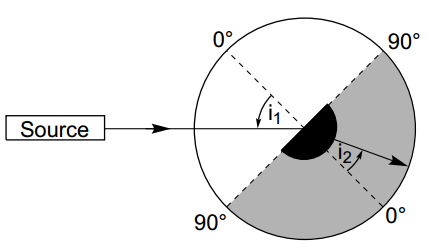
\includegraphics[width=0.4\textwidth]{Images/Schema_exp2.PNG}
\end{center}
\end{multicols}


\begin{center}
    \begin{tabular}{|C{0.1}|C{0.04}|C{0.04}|C{0.04}|C{0.04}|C{0.04}|C{0.04}|C{0.04}|C{0.04}|C{0.04}|C{0.04}|C{0.04}|C{0.04}|C{0.04}|C{0.04}|}
    \hline
        Angle $i_1$ (en $\degree$) & 0 & 5 & 10 & 15 & 20 & 25 & 30 & 35 & 40 & 45 & 50 & 60 & 70 & 80 \\
        \hline
        Angle $i_2$ (en $\degree$) & 0 & 3,5 & 7 & 10 & 13,5  & 16,5 & 20 & 23 & 25,5 & 28,5 & 31 & 36 & 39 & 41,5    \\
        \hline
        $\sin\left(i_1\right)$ & 0 & 0,09 & 0,17 & 0,26 & 0,34  & 0,42  & 0,50 & 0,57 & 0,64 & 0,71 & 0,77 & 0,87 & 0,94  & 0,98 \\
        \hline
        $\sin\left(i_2\right)$ & 0 & 0,06 & 0,12 & 0,17  & 0,23  & 0,28 & 0,34 & 0,39  & 0,43 & 0,48  & 0,52 & 0,58  & 0,63 & 0,66 \\
        \hline
        $\frac{i_1}{i_2}$ & non défini & 1,48 & 1,49 & 1,49 & 1,50 & 1,51 & 1,52 & 1,54 & 1,56 & 1,58 & 1,61 & 1,68 & 1,78 & 1,92  \\
        \hline
       $\frac{\sin\left(i_1\right)}{\sin\left(i_2\right)}$ & non defini & 1,6 & 1,5 & 1,5 & 1,5 & 1,5  & 1,5 &1,5  &1,5  &  1,5& 1,5 & 1,5  & 1,5 & 1,5  \\
        \hline
    \end{tabular}
\end{center}

\subsubsection{Exploitation des résultats}
\question{\`{A} partir des résultats expérimentaux, tracer sur le papier millimétré $i_2$ en fonction de $i_1$.}{\begin{center}
    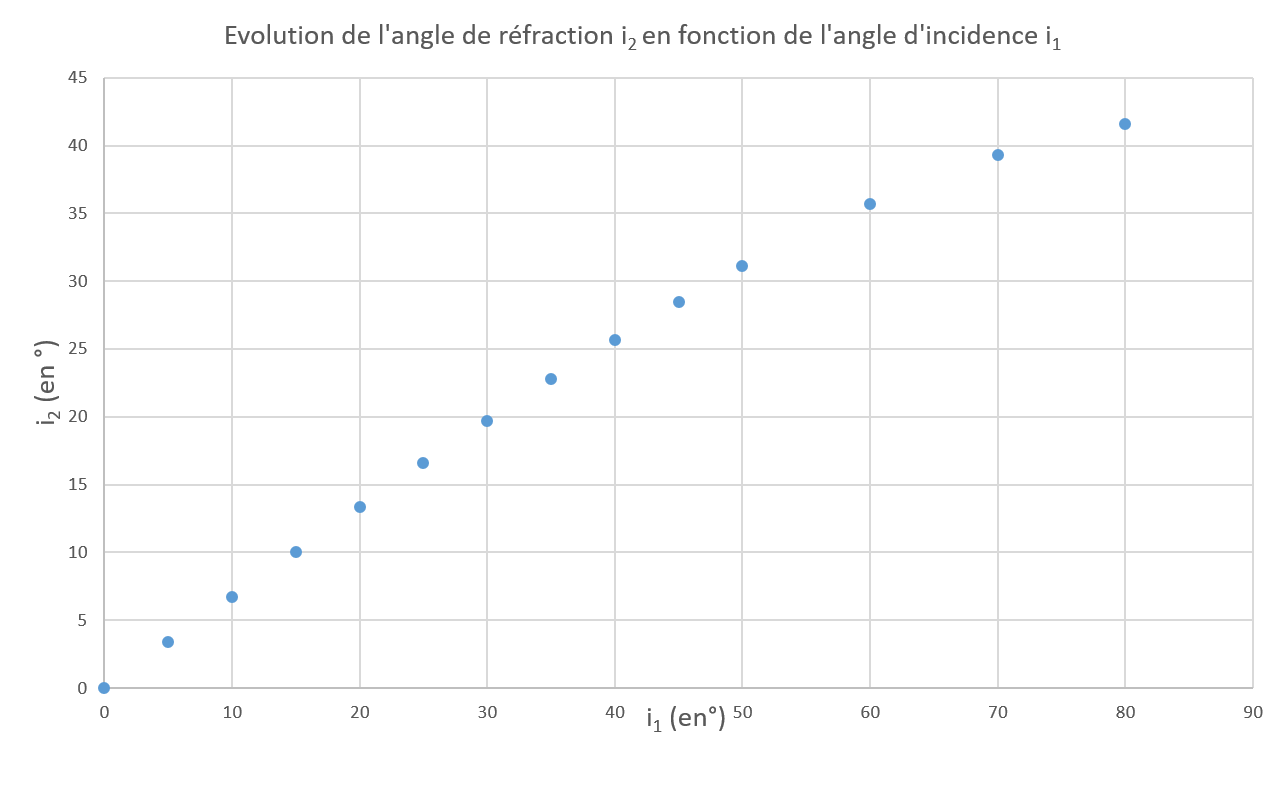
\includegraphics[scale=0.5]{Images/Refraction_i2vsi1.png}
\end{center}}{0}
%\\
\question{Johannes Kepler avait-il raison ?}{Oui à faible angle d'incidence, les angles $i_1$ et $i_2$ sont proportionnels comme on peut le voir sur le graphique ci-dessus.}{0}
\\
\question{Aller chercher le fichier \og TP9\_FeuilleCalculRefraction\_NomClasse\fg~sur l'ENT, dans l'espace documentaire de la classe.}{Fais en classe.}{0}
\\
\question{Reporter les valeurs de $i_1$ et de $i_2$ dans le tableau Excel. Convertir les angles $i_1$ et $i_2$ en radian (rad). Puis calculer les sinus de ces angles en utilisant la fonction SINUS() du tableur Excel.}{Fais en classe.}{0}
\\
\question{Tracer le graphique $\sin(i_2)=f(\sin(i_1))$ puis imprimez-le et coller-le sur votre compte-rendu.}{\begin{center}
    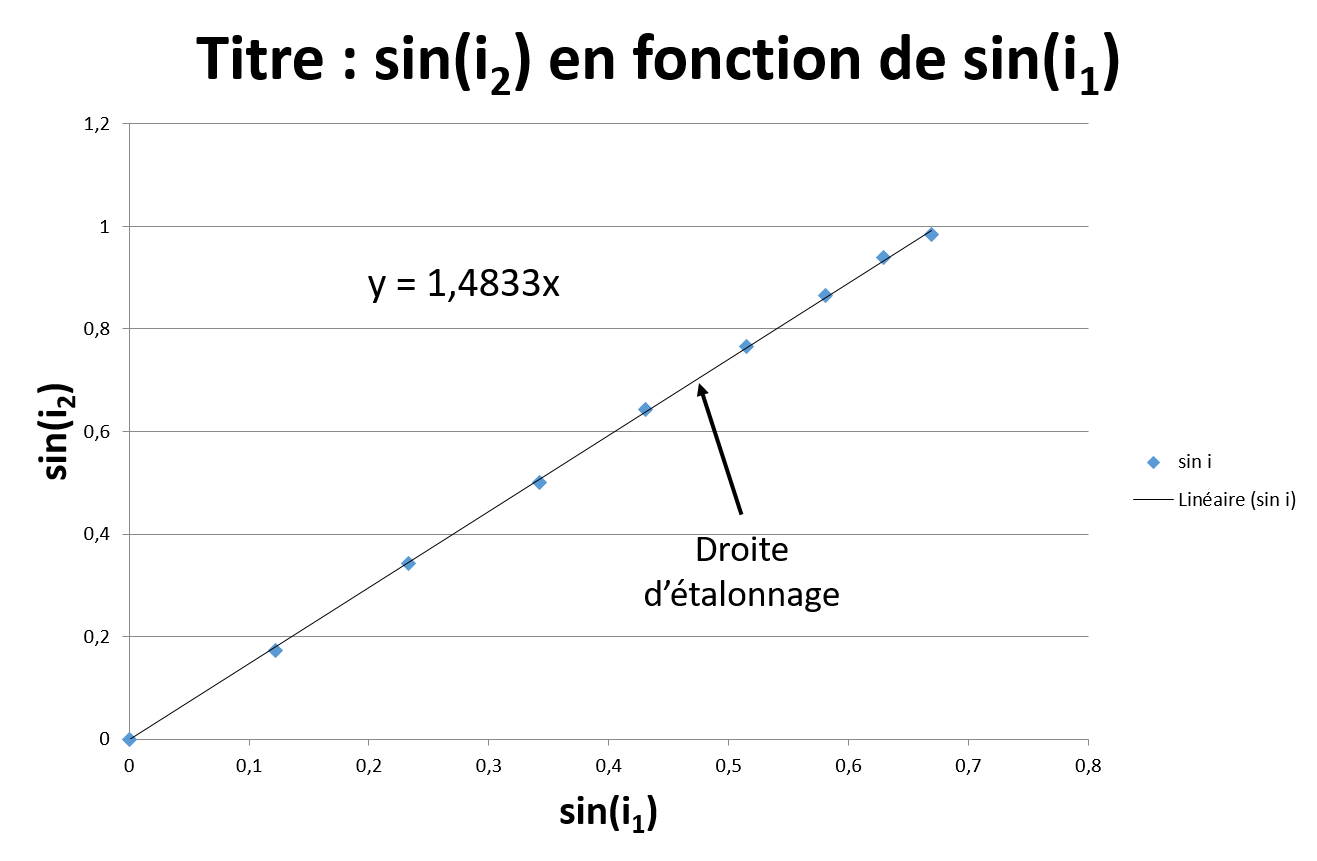
\includegraphics[scale=0.5]{Images/Refraction_resultats.png}
\end{center}}{0}
%\\
\question{En déduire qui de Kepler ou Descartes a énoncé la loi la plus valable. Justifier la réponse.}{C'est bien sûr Descartes car sa loi est valable pour n'importe quel angle d'incidence $i_1$, tandis que la loi énoncée par Kepler n'est valable que pour des petits angles d'incidence.}{0}
\\
On suppose que $\frac{\sin\left(i_2\right)}{\sin\left(i_1\right)} = \frac{n_2}{n_1}$ où $n_1$ et $n_2$ sont des nombres sans unités appelés \textcolor{red}{indices de réfraction}.\\
\question{En utilisant les fonctionnalités d’Excel (voir fiche méthode), déterminer une valeur expérimentale de $\frac{n_2}{n_1}$.}{A l'aide de l'équation de la droite d'étalonnage, on lit : $\frac{n_2}{n_1}=1,48$.}{0}

\begin{tcolorbox}[colback=red!5!white,colframe=red!75!black,title=\textbf{Loi de Snell-Descartes pour la réfraction : }]
\texteTrouMultiLignes{L'angle d'incidence $i_1$ est relié à l'angle de réfraction $i_2$ par la formule suivante :\begin{empheq}[box=\fbox]{equation*}
    n_1\sin\left(i_1\right)=n_2\sin\left(i_2\right)
\end{empheq}.}{2}
\end{tcolorbox}

\question{En sachant que $n_1=n_{air}=1$, déterminer la valeur de $n_2=n_{plexiglas}$.}{On détermine directement : 
\begin{equation*}
    n_{plexiglas} = 1,48\times n_{air} = 1,48
\end{equation*}
}{0}



%\newpage
%\papiermillimetre
  %
\modeCorrection

%%%% début de la page
\renewcommand{\thesection}{\textcolor{red}{Partie \Roman{section} -}}
\renewcommand{\thesubsection}{\textcolor{red}{\Roman{section}.\arabic{subsection}}}
\renewcommand{\thesubsubsection}{\textcolor{red}{\Roman{section}.\arabic{subsection}.\alph{subsubsection}}}

\setcounter{section}{0}
\setcounter{document}{0}
\sndEnTeteTPDix

\begin{center}
\begin{mdframed}[style=titr, leftmargin=60pt, rightmargin=60pt, innertopmargin=7pt, innerbottommargin=7pt, innerrightmargin=8pt, innerleftmargin=8pt]

\begin{center}
\large{\textbf{TP 10 : L'apparition d'un arc-en-ciel
}}
\end{center}
\end{mdframed}
\end{center}

\begin{tableauCompetences}
    REA & Réaliser un montage à l'aide d'un protocole expérimental & & & & \\
    \hline
    APP & Exploiter un spectre d'émission & & & & \\   
    \hline 
    REA & Connaître et exploiter les lois de Snell-Descartes & & & & \\
    \hline 
    COM & Rendre compte de façon écrite & & & & \\
    \hline
    VAL & Analyser l’ensemble des résultats de façon critique  & & & &
\end{tableauCompetences}


%%%% objectifs
\begin{tcolorbox}[colback=blue!5!white,colframe=blue!75!black,title=Objectifs de la séance :]
\begin{itemize}
    \item Décrire et expliquer qualitativement le phénomène de dispersion de la lumière par un prisme ;
    \item Produire et exploiter des spectres d'émission obtenus à l'aide d'un système dispersif ;
\end{itemize}
\end{tcolorbox}

%%%% Consignes
\begin{tcolorbox}[colback=red!5!white,colframe=red!75!black,title= Consignes :]
\begin{itemize}
    \item Faire attention au matériel lors de son utilisation ;
    \item Produire et rendre un compte rendu écrit de TP par binôme ;
\end{itemize}
\end{tcolorbox}

%%%% contexte
\section{Mise en évidence expérimentale}
\begin{tcolorbox}[colback=orange!5!white,colframe=orange!75!black,title= Expérience d'Isaac Newton :]
\begin{wrapfigure}{r}{0.4\textwidth}
\vspace{-0.6cm}
    \centering
     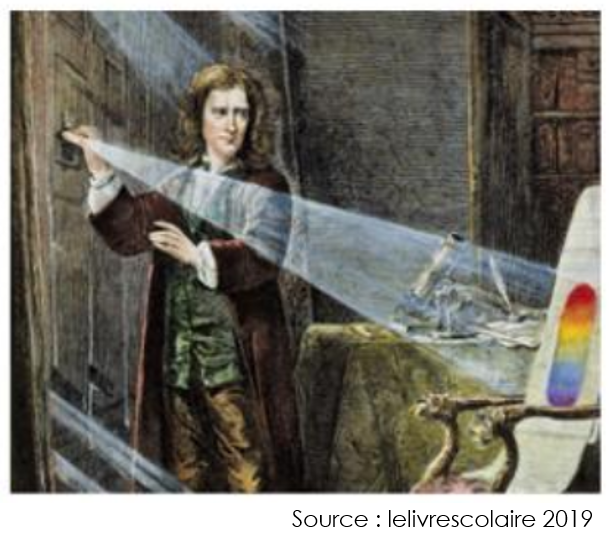
\includegraphics[width=0.4\textwidth]{Images/Isaac_Newton.PNG}
   \end{wrapfigure}
Le physicien Isaac Newton (1643-1727) a mené en 1666 une expérience sur la lumière du Soleil qui allait révolutionner la conception de l'optique que l'on avait à l'époque. Pour cela, il a réalisé une petite ouverture dans son volet afin qu'un fin faisceau lumineux pénètre dans la pièce. Il a alors placé un prisme de verre sur le trajet de la lumière. Il a constaté que la lumière était déviée par le prisme et qu'elle formait sur un écran un dégradé de couleurs allant du rouge au violet, appelé \textcolor{red}{spectre}.\\

\problematique{Quel phénomène permet d'expliquer l'apparition d'un arc-en-ciel ?}
\end{tcolorbox}

\begin{mdframed}[style=autreexo]
\textbf{\bsc{Liste du matériel}}
\begin{multicols}{2}
    \begin{itemize}
    \item Un générateur de tension continue ;
    \item Une lampe à incandescence ;
    \item Une lentille convergente ;
    \item Une fente ;
    \item Un prisme ;
    \item Un écran ;
    \item Une lampe à vapeur de mercure ;
    \item Un filtre rouge et un filtre bleu ;
\end{itemize}
\end{multicols}
\end{mdframed}

\begin{large}
    \textbf{\textcolor{red}{\underline{Travail à réaliser :}}}
\end{large}
\\
\question{\`{A} l'aide du matériel que vous avez à disposition, réaliser la même expérience qu'Isaac Newton. Observe-t'on le même résultat que le physicien ?}{Oui on observe les mêmes résultats que le physicien à savoir la décomposition du spectre de la lumière blanche par le prisme.}{0}
\\
\question{Réaliser un schéma de votre expérience en reproduisant le résultat obtenu.}{\begin{center}
    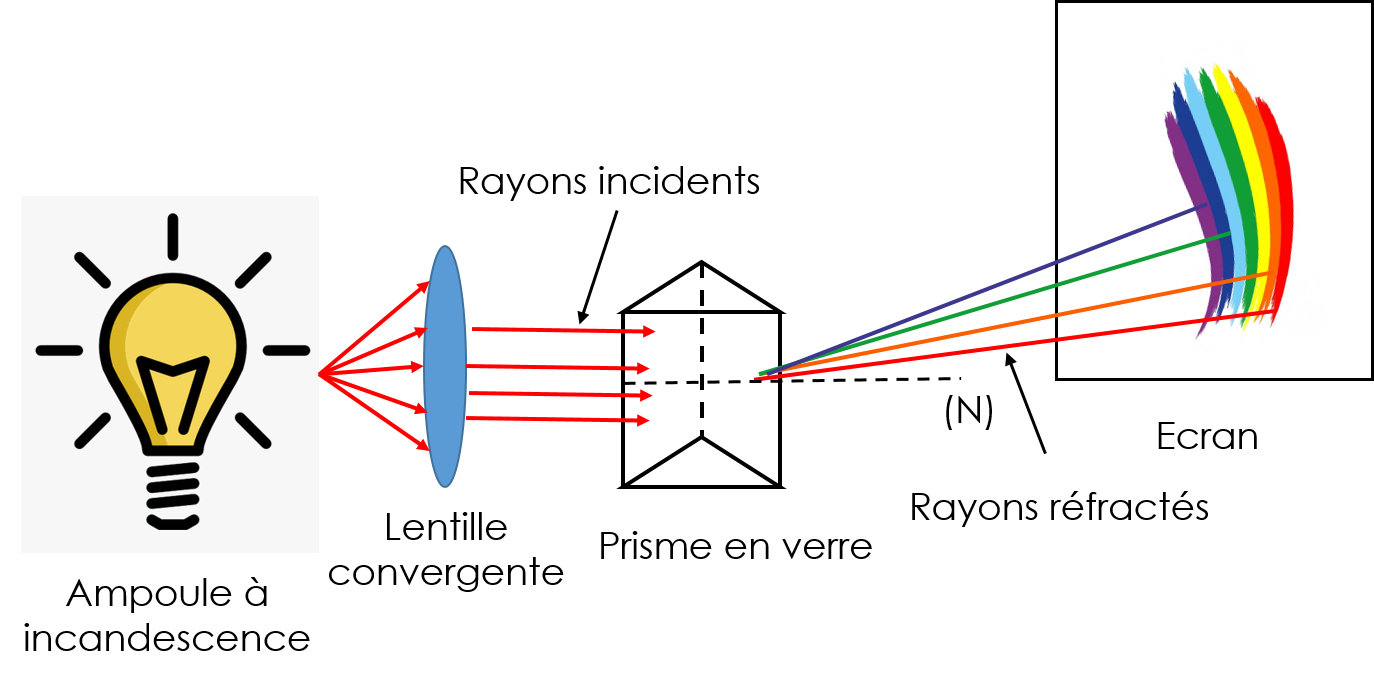
\includegraphics[scale=0.5]{Images/Montage.png}
\end{center}}{0}
%\\
\question{Mettre un filtre rouge devant la sortie de la lampe à incandescence. Réaliser la même expérience avec un filtre bleu. Reproduire le résultat sur un schéma pour chacune des expériences. En déduire l'utilité d'un filtre.}{Le filtre rouge sélectionne la couleur rouge et le filtre bleu sélectionne la lumière bleu. Un filtre permet de sélectionner une radiation particulière. Plus un filtre est sélectif, moins on verra les couleurs qu'il ne sélectionne pas.}{0}
\\
\question{Indiquer quelle radiation est la plus déviée et laquelle est la moins déviée par le prisme.}{Le schéma nous permet de dire que la radiation la plus déviée (par rapport au rayon incident) et la lumière violette (bleue acceptée).}{0}
\\
\question{Au bureau, la même expérience que celle de Newton est réalisée en remplaçant la lampe à incandescence par la lampe à vapeur de mercure. Noter vos observations en réalisant un schéma.}{\begin{center}
    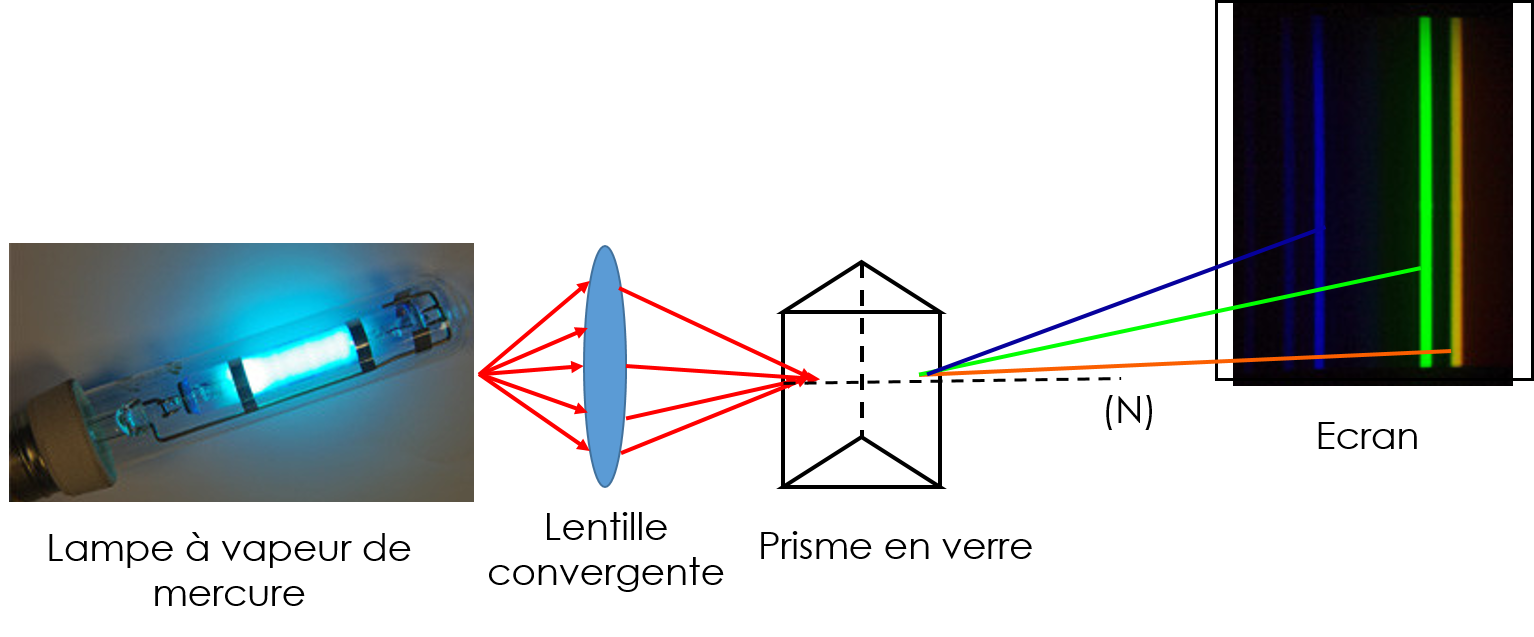
\includegraphics[scale=0.5]{Images/Montage_mercure.png}
\end{center}}{0}
%%%% documents

%\begin{center}
 %   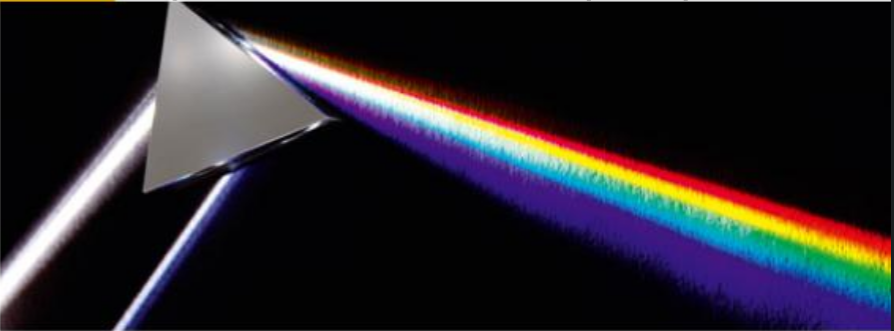
\includegraphics[scale=1.1]{Images/Dispersion.PNG}
%\end{center}

%%%%
%\newpage
\section{Interprétation des résultats}

\begin{doc}{Variation de l'indice optique du verre en fonction de la radiation qui le traverse}
    L'indice optique du verre dépend de la longueur d'onde de la radiation qui le traverse : un verre est un milieu dit \textcolor{red}{dispersif}. Par exemple, pour une radiation rouge, l'indice optique $n_{rouge}=1,510$ et pour une radiation bleue $n_{bleu}=1,520$.
\end{doc}
\begin{large}
    \textbf{\textcolor{red}{\underline{Travail à réaliser :}}}
\end{large}
\\
%\\
\question{Voici un prisme dont l'angle au sommet A vaut 35$\degree$ :
\begin{center}
    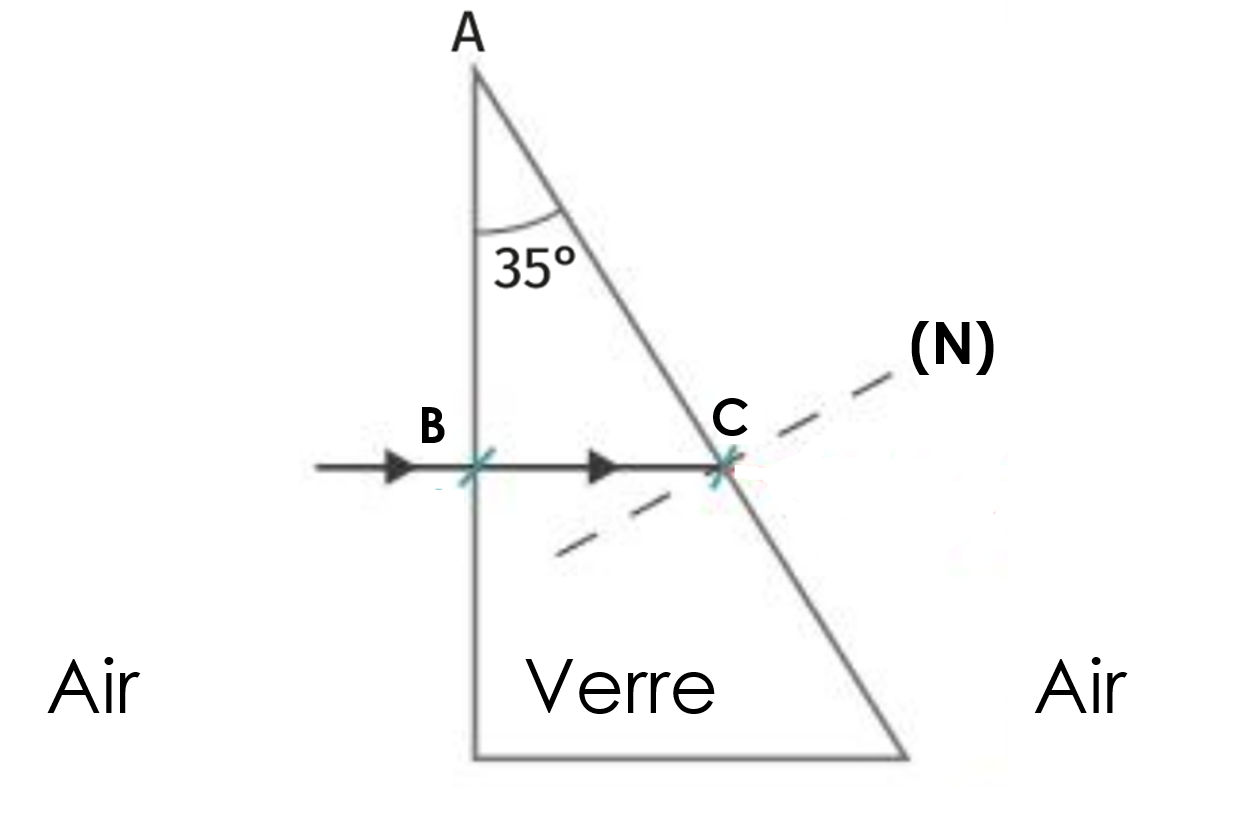
\includegraphics[scale=0.6]{Images/Prisme_exo.PNG}
\end{center}
Indiquer l'angle d'incidence $i_1$ et l'angle de réfraction $i_2$ à l'interface verre-air (c'est-à-dire  au point \textbf{C}).}{\begin{center}
    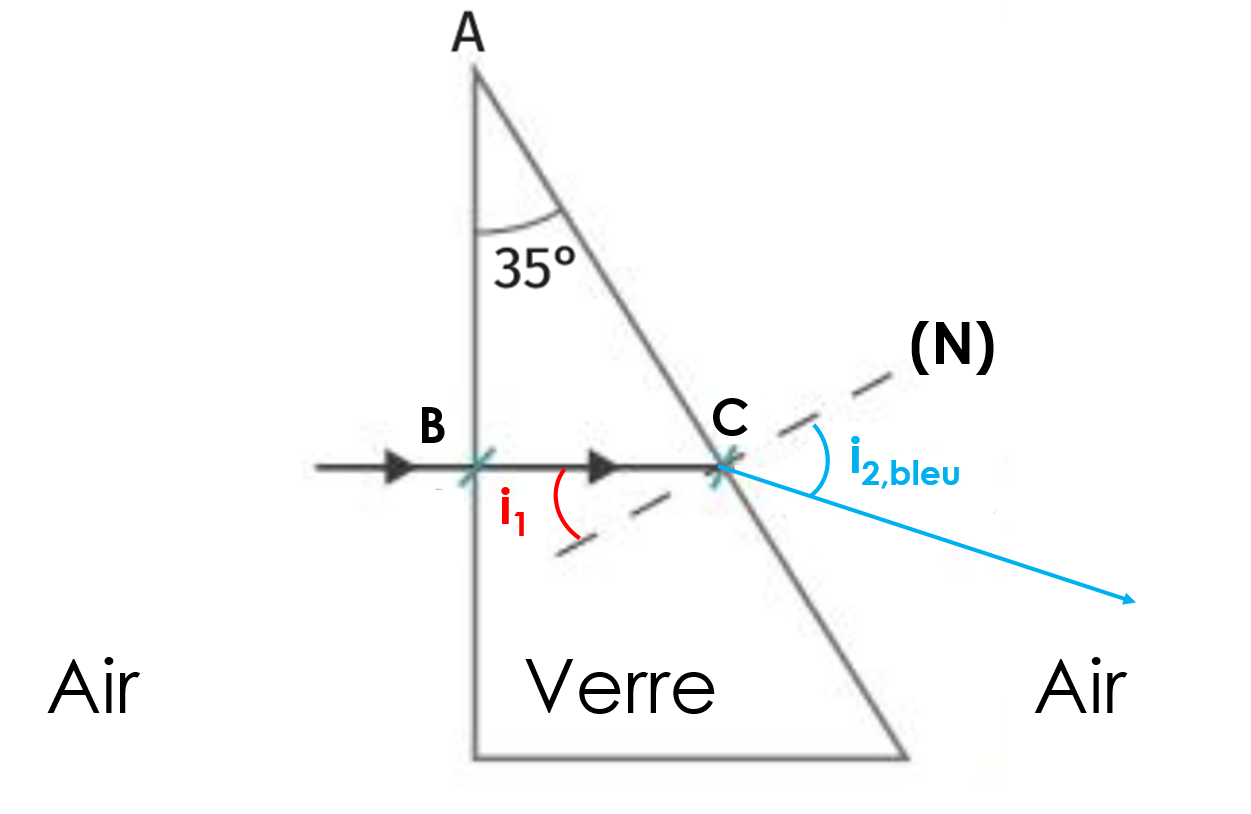
\includegraphics[scale=0.6]{Images/Prisme_correction6.png}
\end{center}}{0}
%\\
%\begin{minipage}{0.47\textwidth}

\begin{facile}{Parcours dispersion}

\question{Rappeler la loi de Snell-Descartes pour la réfraction.}{Les rayons incident et réfracté appartiennent au même plan appelé plan d'incidence. Ces deux rayons sont tels qu'on a la relation : 
\begin{equation*}
    n_1\times \sin\left(i_1\right) = n_2\times \sin\left(i_2\right)
\end{equation*}}{0}
%\\
\question{Justifier que le rayon n'est pas dévié au point \textbf{B}.}{L'angle d'incidence au point \textbf{B} vaut $0\degree$, l'angle de réfraction est donc nul d'après la loi de Descartes sur la réfraction :
\begin{equation*}
    n_{verre}\sin(0) = 0 = n_{air}\sin(i_2)
\end{equation*}
Donc $\sin(i_2)=0$ donc  $i_2=0$.}{0}
\\
\question{Déterminer l'angle de réfraction de la lumière bleue en sachant que l'angle d'incidence au point \textbf{C} vaut 35$\degree$.}{D'après la loi de Descartes sur la réfraction :
\begin{equation*}
    n_{\text{bleu}}\times \sin\left(i_1\right) = n_{air}\times \sin\left(i_{2,\text{bleu}}\right)
\end{equation*}
On en déduit que : 
\begin{equation*}
    \sin\left(i_{2,\text{bleu}}\right) = \frac{n_{\text{bleu}}}{n_{air}}\times \sin\left(i_1\right)
\end{equation*}
Et donc que : 
\begin{align*}
    i_{2,\text{bleu}} &= \arcsin\left(\frac{n_{\text{bleu}}}{n_{air}}\times \sin\left(i_1\right) \right) \\
     i_{2,\text{bleu}} &= \arcsin\left(\frac{1,520}{1,00}\times \sin\left(35\degree\right) \right) \\
     i_{2,\text{bleu}} &= 60,7\degree
\end{align*}}{0}

\end{facile}
%\end{minipage}
%
%\hspace{0.05\textwidth}
%\begin{minipage}{0.47\textwidth}
%\vspace{-2.5cm}

\begin{difficile}{Parcours Newton}
\question{Tracer les rayons rouge et bleu en indiquant précisément les angles de réfraction $i_{2,rouge}$ et $i_{2,bleu}$.}{Merci à Gabrielle Reniez et Laura Leung pour cette très belle démonstration ! 
\begin{center}
    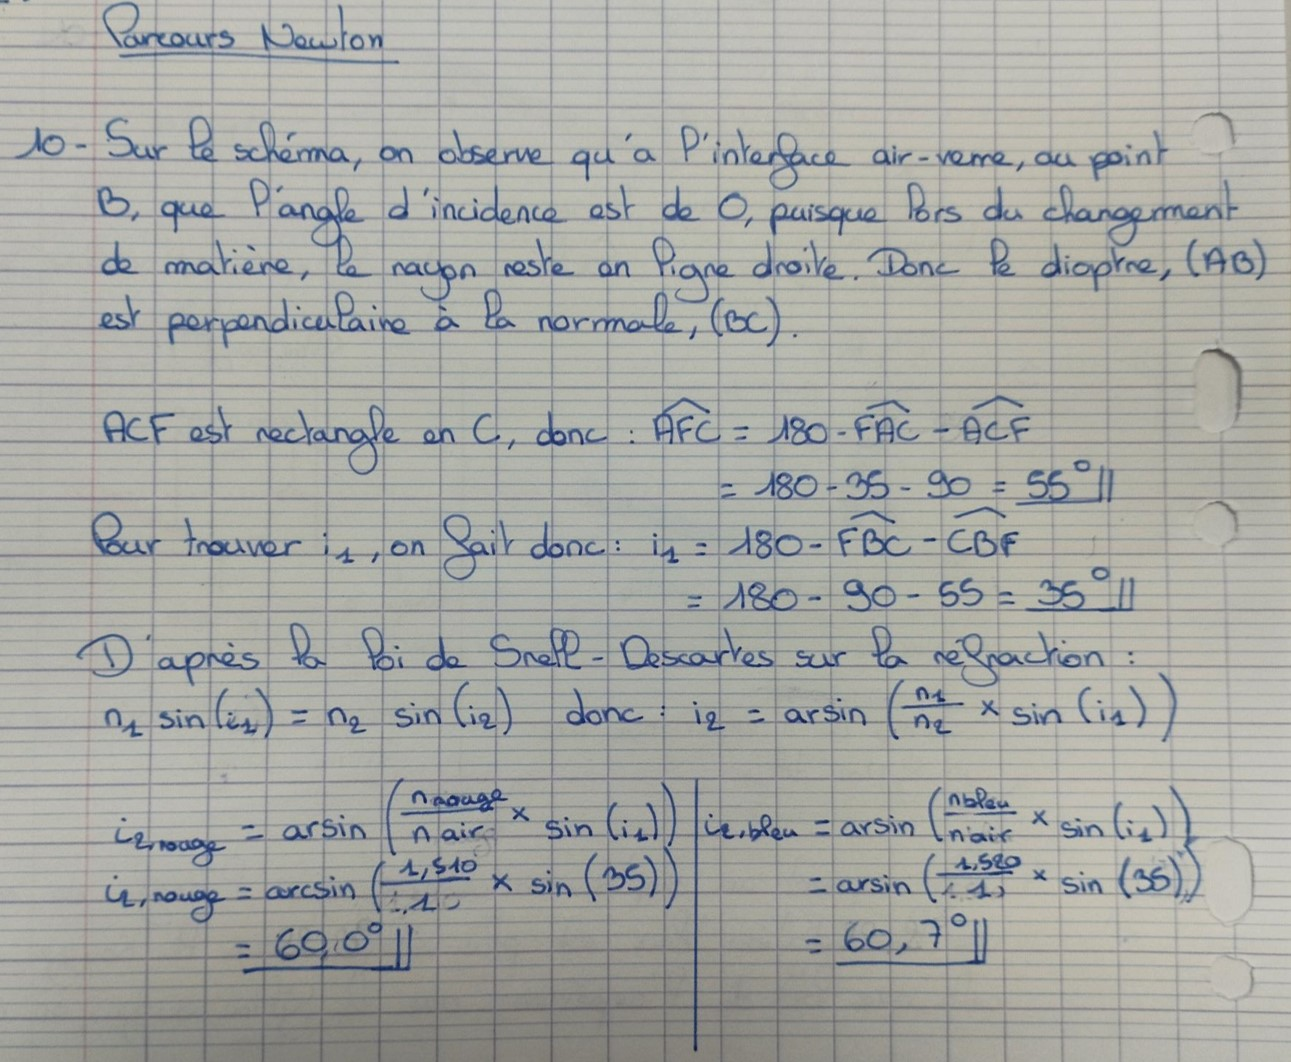
\includegraphics[scale=0.7]{Images/Correction_Newton.jpg}
\end{center}
On peut alors tracer les rayons bleu et rouge :
\begin{center}
    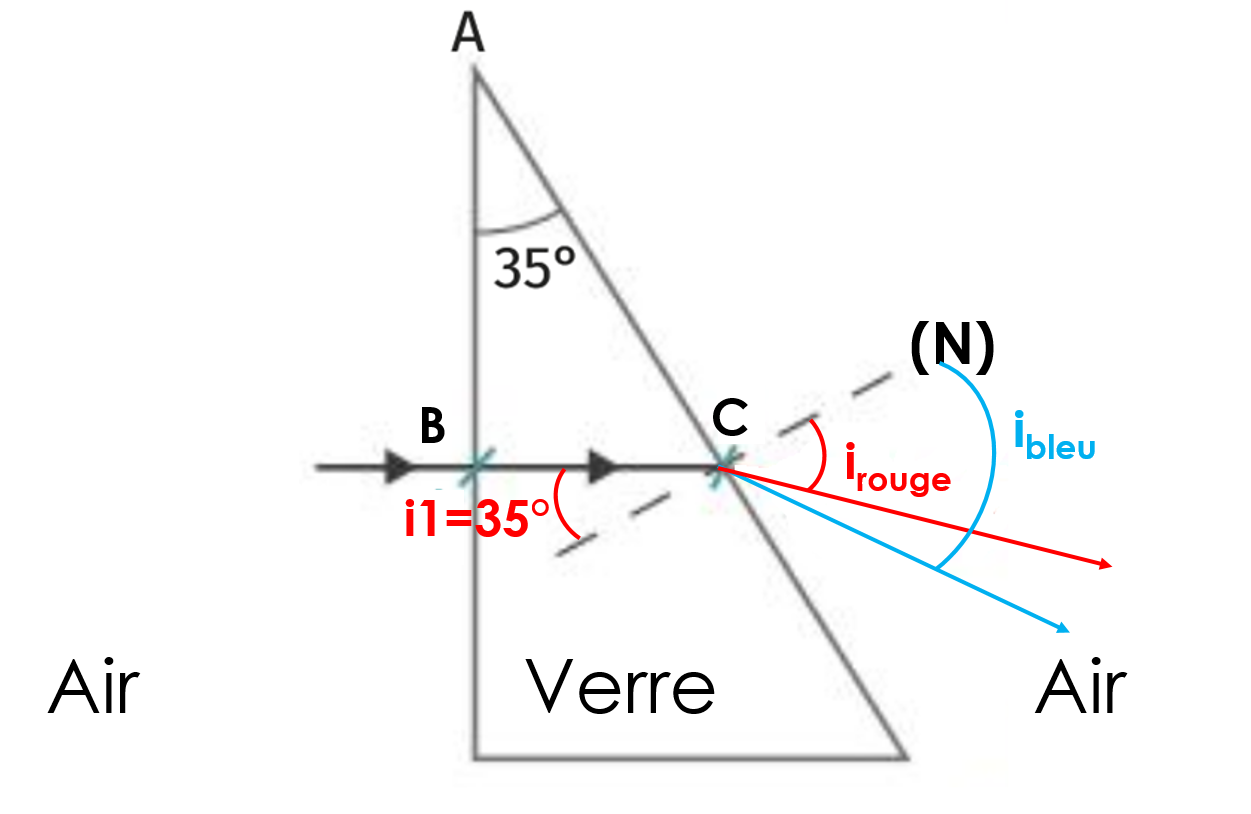
\includegraphics[scale=0.6]{Images/Prisme_correction10.png}
\end{center}}{0}
\end{difficile}
%\hfill
%\end{minipage}

\newpage

\begin{difficile}{\large Bilan de l'activité sur la dispersion}
\vspace{0.5cm}
\question{Quel phénomène permet d'expliquer la déviation de la lumière par le prisme ?}{Il s'agit de la réfraction. Lorsque l'indice optique d'un milieu dépend de la longueur d'onde (la couleur autrement dit) de la lumière, l'angle de réfraction va changer suivant la couleur de la lumière. Le milieu est alors dit \underline{dispersif}.}{0}
\\
\question{Lors de la formation d'un arc-en-ciel, quel élément joue un rôle de prisme ?}{Il s'agit des gouttes d'eau composant la pluie.}{0}
    \texteTrouMultiLignes{~}{15}
\end{difficile}

  %\modeCorrection

%%%% début de la page
\renewcommand{\thesection}{\textcolor{red}{Partie \Roman{section} -}}
\renewcommand{\thesubsection}{\textcolor{red}{\Roman{section}.\arabic{subsection}}}
\renewcommand{\thesubsubsection}{\textcolor{red}{\Roman{section}.\arabic{subsection}.\alph{subsubsection}}}

\setcounter{section}{0}
\setcounter{document}{0}
\sndEnTeteTPDix

\nomPrenomClasse

\begin{center}
\begin{mdframed}[style=titr, leftmargin=60pt, rightmargin=60pt, innertopmargin=7pt, innerbottommargin=7pt, innerrightmargin=8pt, innerleftmargin=8pt]

\begin{center}
\large{\textbf{TP 10 : L'apparition d'un arc-en-ciel
}}
\end{center}
\end{mdframed}
\end{center}

\begin{tableauCompetences}
    \hline
    APP & Exploiter un spectre d'émission & & & & \\   
    \hline 
    REA & Connaître et exploiter les lois de Snell-Descartes & & & & \\
    \hline 
    COM & Rendre compte de façon écrite & & & & 
\end{tableauCompetences}


%%%% objectifs
\begin{tcolorbox}[colback=blue!5!white,colframe=blue!75!black,title=Objectifs de la séance :]
\begin{itemize}
    \item Décrire et expliquer qualitativement le phénomène de dispersion de la lumière par un prisme ;
    \item Exploiter des spectres d'émission obtenus à l'aide d'un système dispersif ;
\end{itemize}
\end{tcolorbox}

%%%% Consignes
\begin{tcolorbox}[colback=red!5!white,colframe=red!75!black,title= Consignes :]
\begin{itemize}
    \item Rédiger un compte-rendu individuel ;
    \item Interdiction de se déplacer dans la salle sauf autorisation explicite ;
\end{itemize}
\end{tcolorbox}

%%%% contexte
\section{Mise en évidence expérimentale}
\begin{tcolorbox}[colback=orange!5!white,colframe=orange!75!black,title= Expérience d'Isaac Newton :]
\begin{wrapfigure}{r}{0.4\textwidth}
\vspace{-0.6cm}
    \centering
     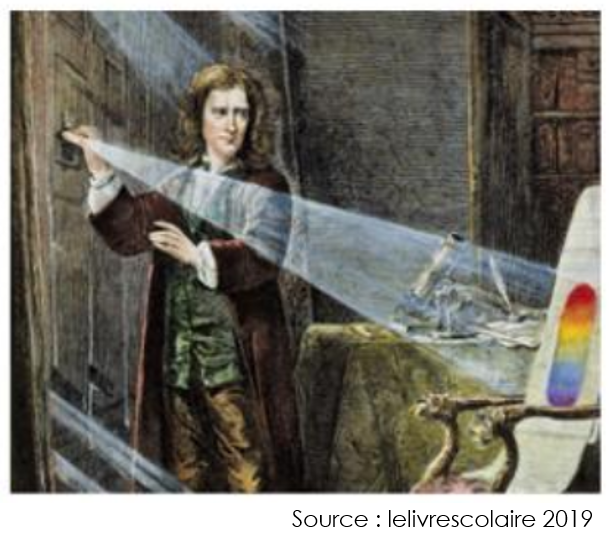
\includegraphics[width=0.4\textwidth]{Images/Isaac_Newton.PNG}
   \end{wrapfigure}
Le physicien Isaac Newton (1643-1727) a mené en 1666 une expérience sur la lumière du Soleil qui allait révolutionner la conception de l'optique que l'on avait à l'époque. Pour cela, il a réalisé une petite ouverture dans son volet afin qu'un fin faisceau lumineux pénètre dans la pièce. Il a alors placé un prisme de verre sur le trajet de la lumière. Il a constaté que la lumière était déviée par le prisme et qu'elle formait sur un écran un dégradé de couleurs allant du rouge au violet, appelé \textcolor{red}{spectre}.\\

\problematique{Quel phénomène permet d'expliquer l'apparition d'un arc-en-ciel ?}
\end{tcolorbox}

\begin{mdframed}[style=autreexo]
\textbf{\bsc{Liste du matériel}}
\begin{multicols}{2}
    \begin{itemize}
    \item Un générateur de tension continue ;
    \item Une lampe à incandescence ;
    \item Une lentille convergente ;
    \item Une fente ;
    \item Un prisme ;
    \item Un écran ;
    \item Une lampe à vapeur de mercure ;
    \item Un filtre rouge et un filtre bleu ;
\end{itemize}
\end{multicols}
\end{mdframed}

\begin{large}
    \textbf{\textcolor{red}{\underline{Travail à réaliser (20min):}}}
\end{large}
\\
\question{Au bureau, la même expérience qu'Isaac Newton a été réalisée. Observe-t'on le même résultat que le physicien ?}{Oui on observe bien le même résultat que le physicien à savoir l'apparition du spectre de la lumière blache.}{0}
\\
\question{Réaliser un schéma de l'expérience en reproduisant le résultat obtenu. On utilisera bien le vocabulaire appris dans le cours (rayon incident, réfléchi, réfracté).}{\begin{center}
    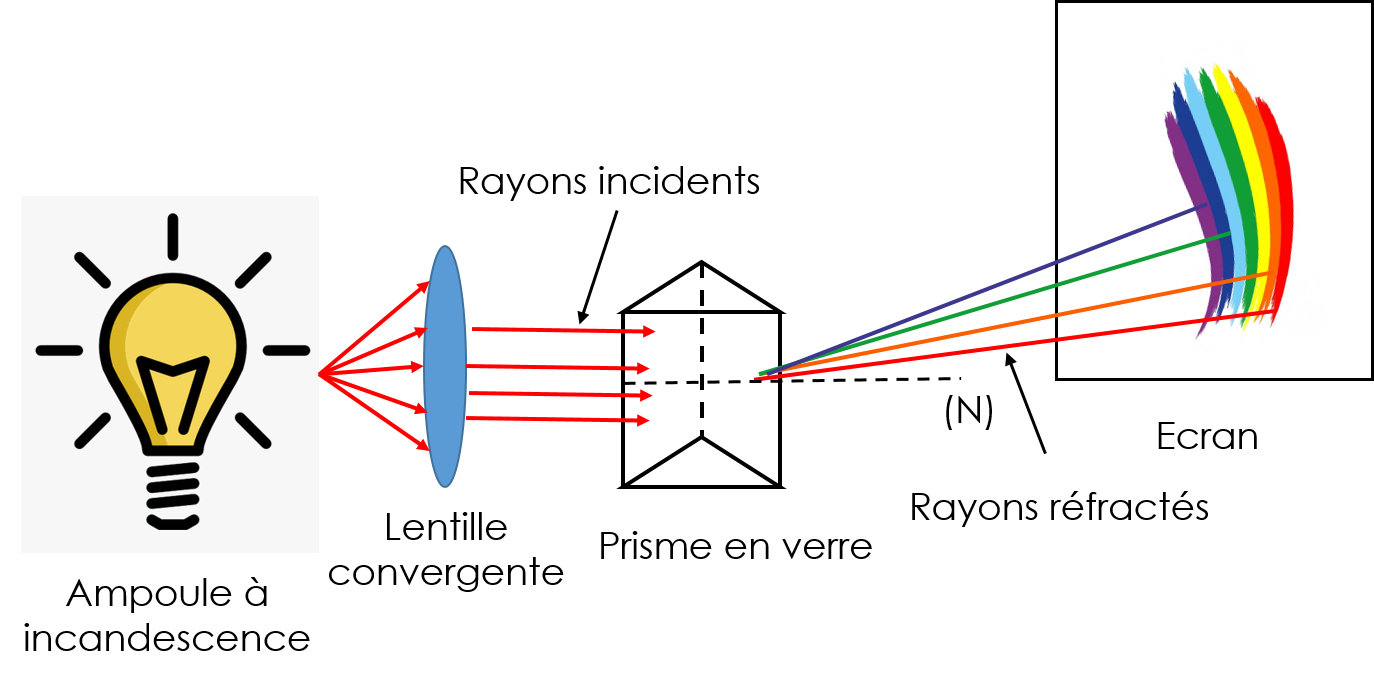
\includegraphics[scale=0.6]{Images/Montage.png}
\end{center}}{0}
%\\
\question{On définit l'angle de déviation comme l'angle entre le rayon arrivant sur le prisme et le rayon réfracté à la sortie du prisme. Indiquer quelle radiation est la plus déviée et laquelle est la moins déviée par le prisme.}{En regardant le schéma, on peut voir que le rayon violet est celui le plus dévié et le rouge est celui le moins dévié.}{0}
\\
%\question{Mettre un filtre rouge devant la sortie de la lampe à incandescence. Réaliser la même expérience avec un filtre bleu. Reproduire le résultat sur un schéma pour chacune des expériences. En déduire l'utilité d'un filtre.}{}{0}
%\\
\question{On remplace la lampe à incandescence par la lampe à vapeur de mercure. Indiquer la différence avec le spectre obtenu dans l'expérience précédente.}{\begin{center}
    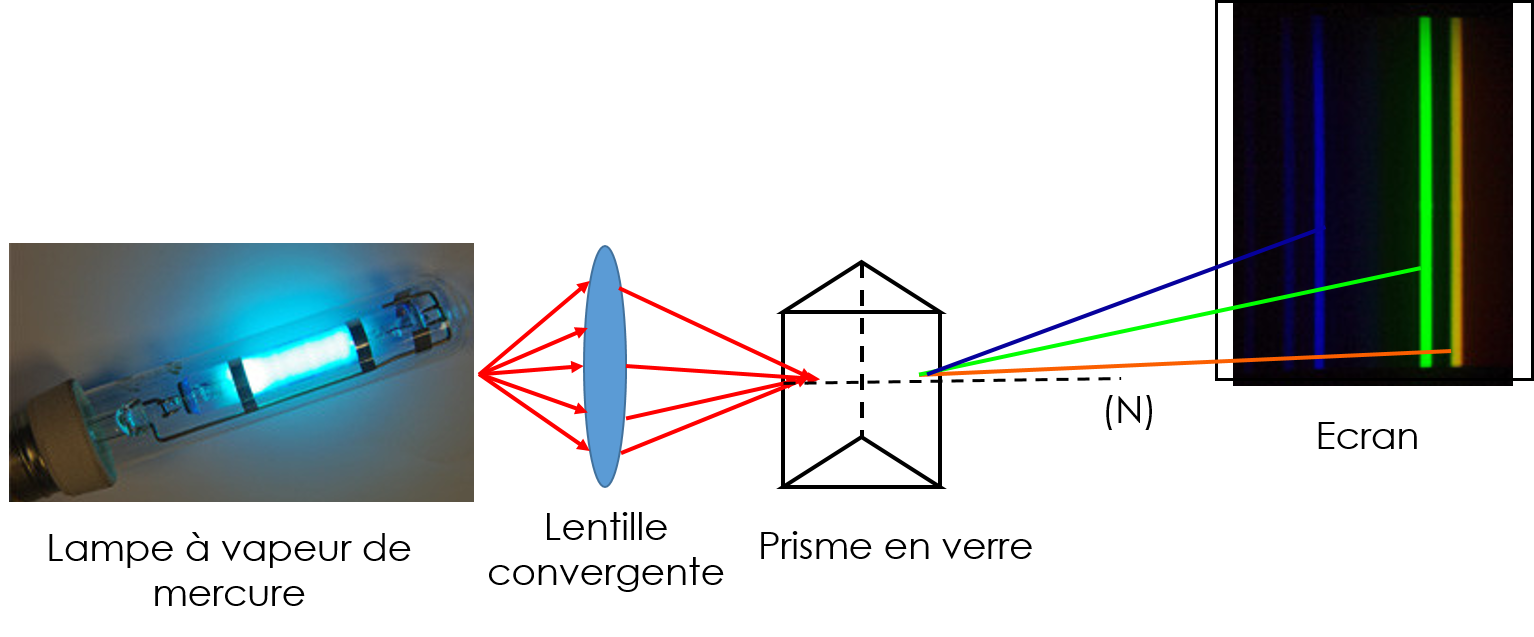
\includegraphics[scale=0.6]{Images/Montage_mercure.png}
\end{center}
On voit qu'il y a moins de couleurs dans le spectre de la lampe à vapeur de mercure que dans le spectre de la lumière blanche.}{0}
%%%% documents

\begin{center}
    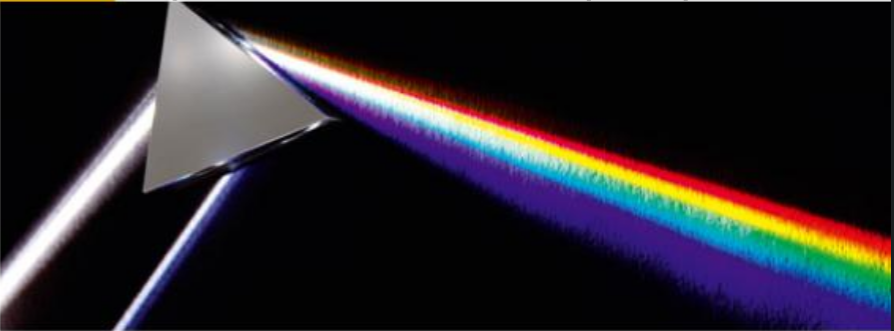
\includegraphics[scale=1.1]{Images/Dispersion.PNG}
\end{center}

%%%%
%\newpage
\section{Interprétation des résultats}

\begin{doc}{Variation de l'indice optique du verre en fonction de la radiation qui le traverse}
    L'indice optique du verre dépend de la longueur d'onde de la radiation qui le traverse : un verre est un milieu dit \textcolor{red}{dispersif}. Par exemple, pour une radiation rouge, l'indice optique $n_{rouge}=1,510$ et pour une radiation bleue $n_{bleu}=1,520$.
\end{doc}
\begin{large}
    \textbf{\textcolor{red}{\underline{Travail à réaliser (30min):}}}
\end{large}
\\
%\\
\question{Voici un prisme dont l'angle au sommet A vaut 35$\degree$ :
\begin{center}
    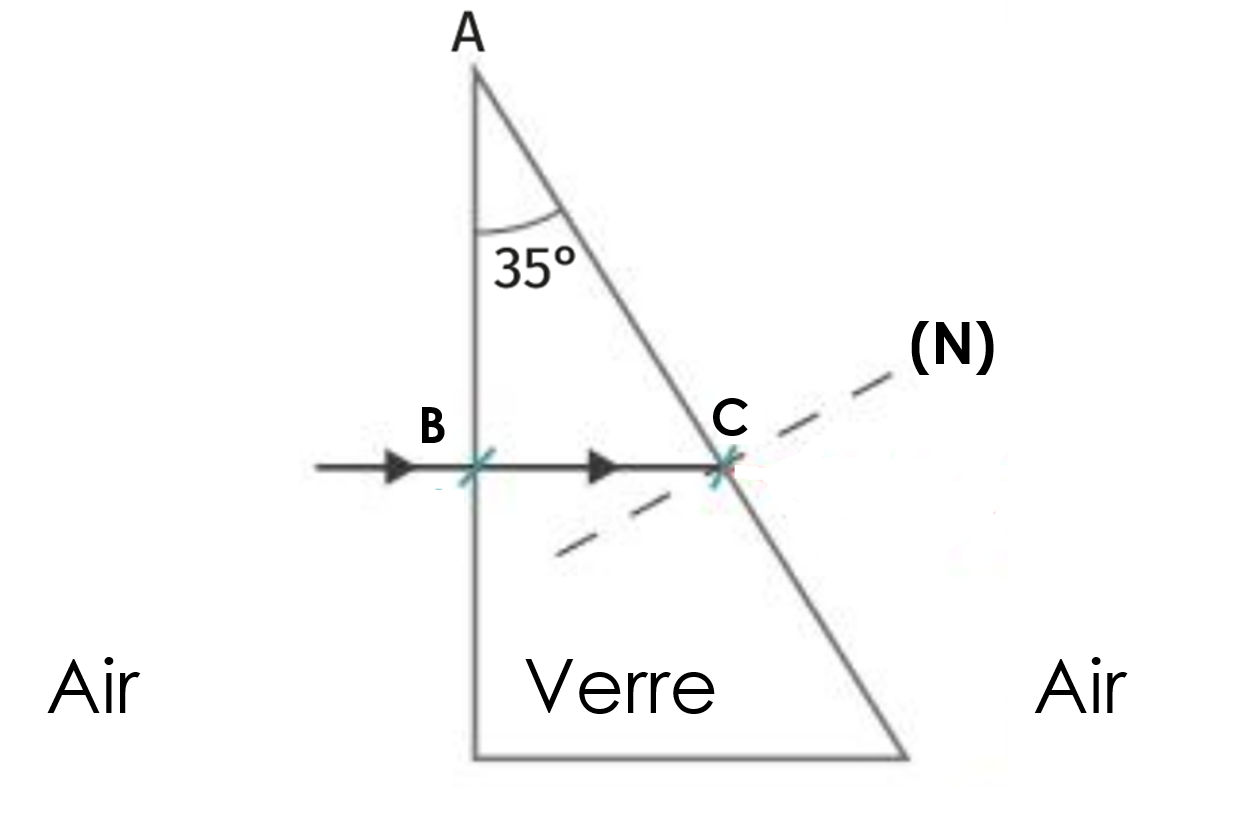
\includegraphics[scale=0.6]{Images/Prisme_exo.PNG}
\end{center}
Tracer le rayon réfléchi à l'interface verre-air (c'est-à-dire  au point \textbf{C}). Indiquer sur le schéma l'angle d'incidence $i_1$ et l'angle de réflexion $r$ en ce point.}{\begin{center}
    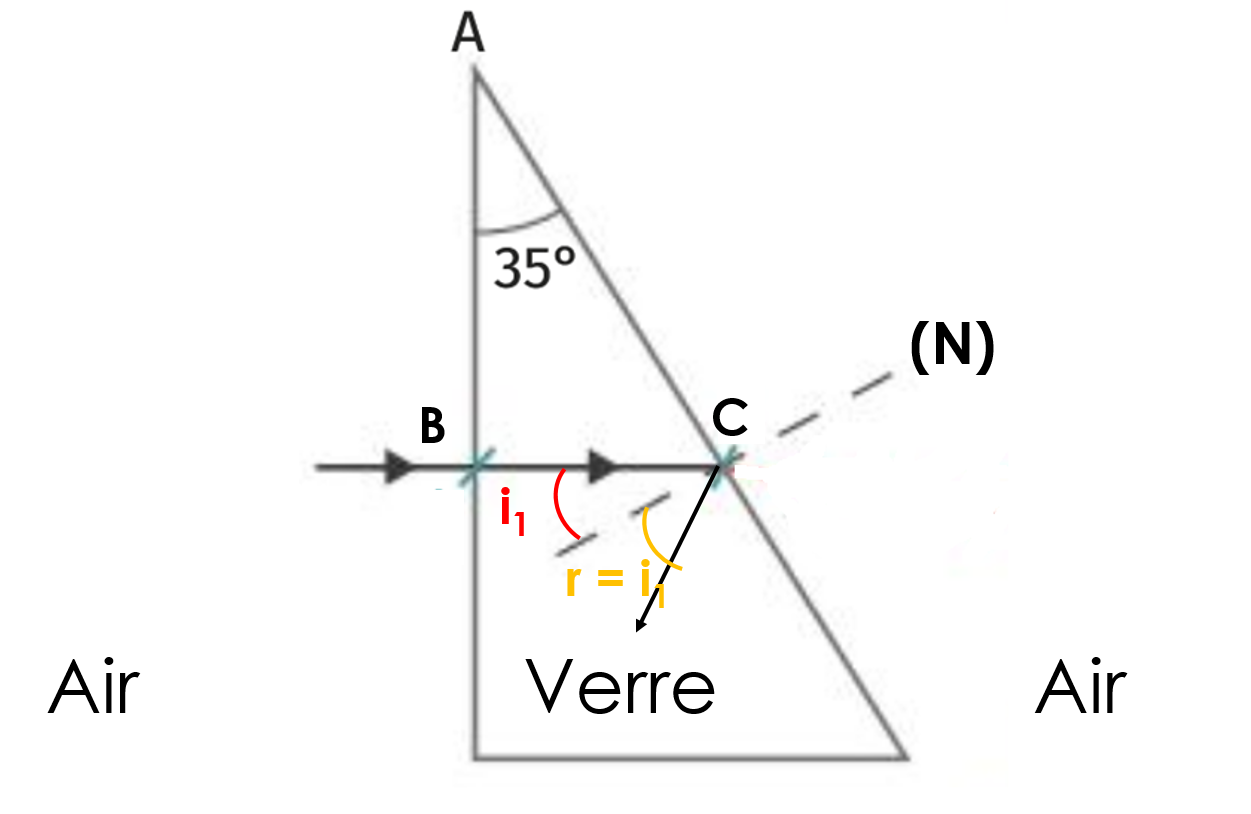
\includegraphics[scale=0.6]{Images/Prisme_correction5.png}
\end{center}}{0}
%\\
%\begin{minipage}{0.47\textwidth}

\begin{facile}{Parcours dispersion}

\question{Rappeler la loi de Snell-Descartes pour la réfraction.}{Les rayons incident et réfracté appartiennent au même plan appelé plan d'incidence. Ces deux rayons sont tels qu'on a la relation : 
\begin{equation*}
    n_1\times \sin\left(i_1\right) = n_2\times \sin\left(i_2\right)
\end{equation*}}{0}
%\\
\question{Justifier que le rayon n'est pas dévié au point \textbf{B}.}{L'angle d'incidence au point \textbf{B} vaut $0\degree$, l'angle de réfraction est donc nul d'après la loi de Descartes sur la réfraction :
\begin{equation*}
    n_{verre}\sin(0) = 0 = n_{air}\sin(i_2)
\end{equation*}
Donc $\sin(i_2)=0$ donc  $i_2=0$.}{0}
\\
\question{Déterminer l'angle de réfraction de la lumière bleue en sachant que l'angle d'incidence au point \textbf{C} vaut 35$\degree$.}{D'après la loi de Descartes sur la réfraction :
\begin{equation*}
    n_{\text{bleu}}\times \sin\left(i_1\right) = n_{air}\times \sin\left(i_{2,\text{bleu}}\right)
\end{equation*}
On en déduit que : 
\begin{equation*}
    \sin\left(i_{2,\text{bleu}}\right) = \frac{n_{\text{bleu}}}{n_{air}}\times \sin\left(i_1\right)
\end{equation*}
Et donc que : 
\begin{align*}
    i_{2,\text{bleu}} &= \arcsin\left(\frac{n_{\text{bleu}}}{n_{air}}\times \sin\left(i_1\right) \right) \\
     i_{2,\text{bleu}} &= \arcsin\left(\frac{1,520}{1,00}\times \sin\left(35\degree\right) \right) \\
     i_{2,\text{bleu}} &= 60,7\degree
\end{align*}}{0}
%\\
\question{Tracer le rayon bleu en indiquant l'angle de réfraction $i_{2,bleu}$ sur le schéma.}{\begin{center}
    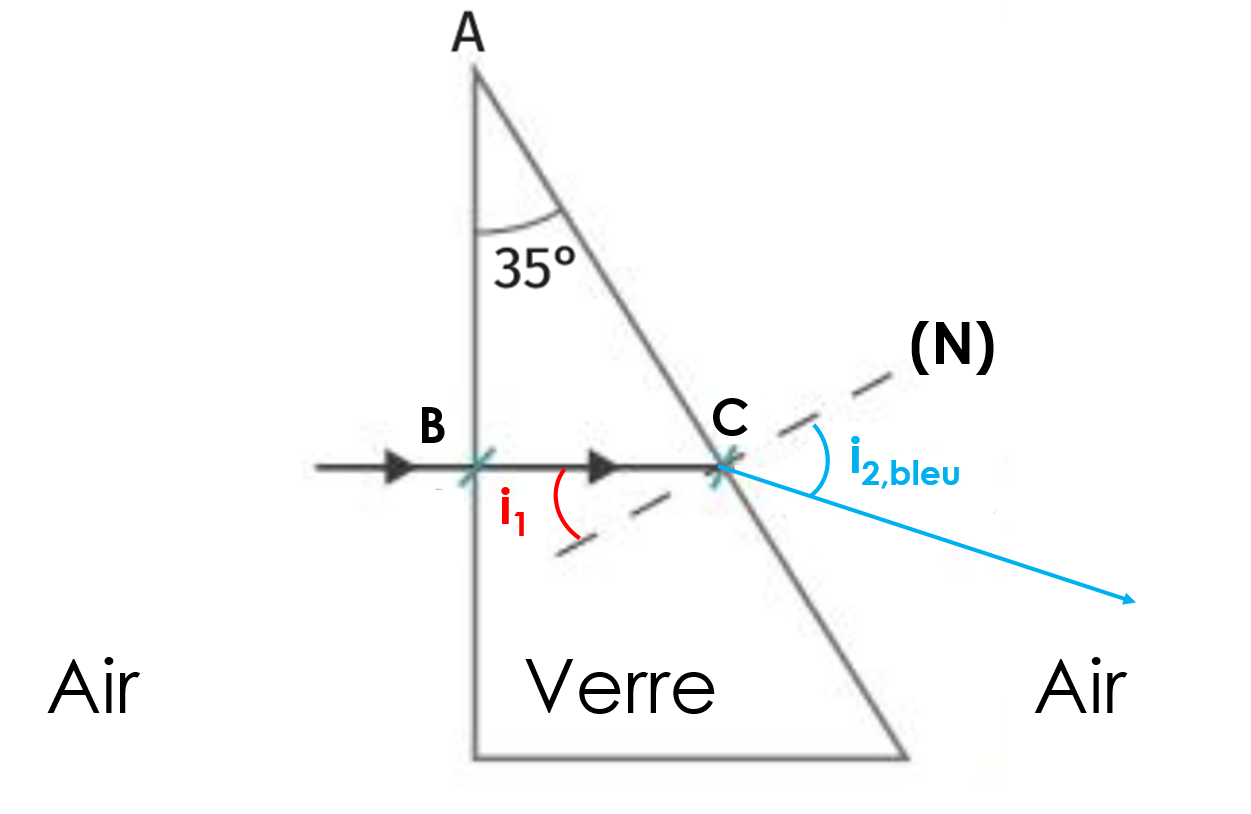
\includegraphics[scale=0.6]{Images/Prisme_correction6.png}
\end{center}}{0}

\end{facile}
%\end{minipage}
%
%\hspace{0.05\textwidth}
%\begin{minipage}{0.47\textwidth}
%\vspace{-2.5cm}

\begin{difficile}{Parcours Newton}
\question{Tracer les rayons rouge et bleu en indiquant précisément les angles de réfraction $i_{2,rouge}$ et $i_{2,bleu}$. Justifier chaque étape de calcul.}{Merci à Gabrielle Reniez et Laura Leung pour cette très belle démonstration ! 
\begin{center}
    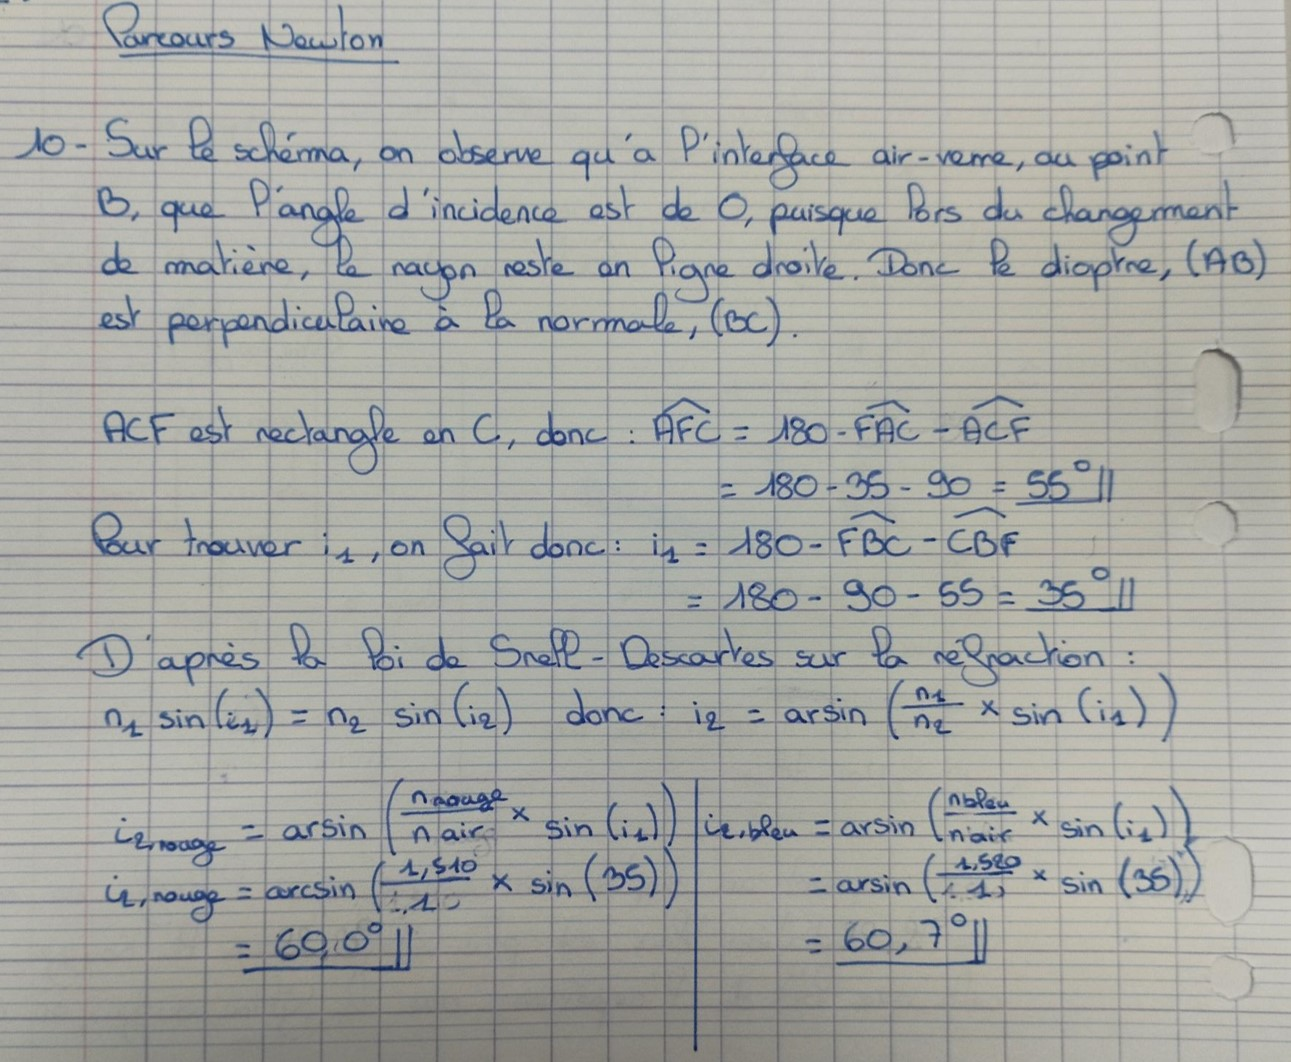
\includegraphics[scale=0.7]{Images/Correction_Newton.jpg}
\end{center}
On peut alors tracer les rayons bleu et rouge :
\begin{center}
    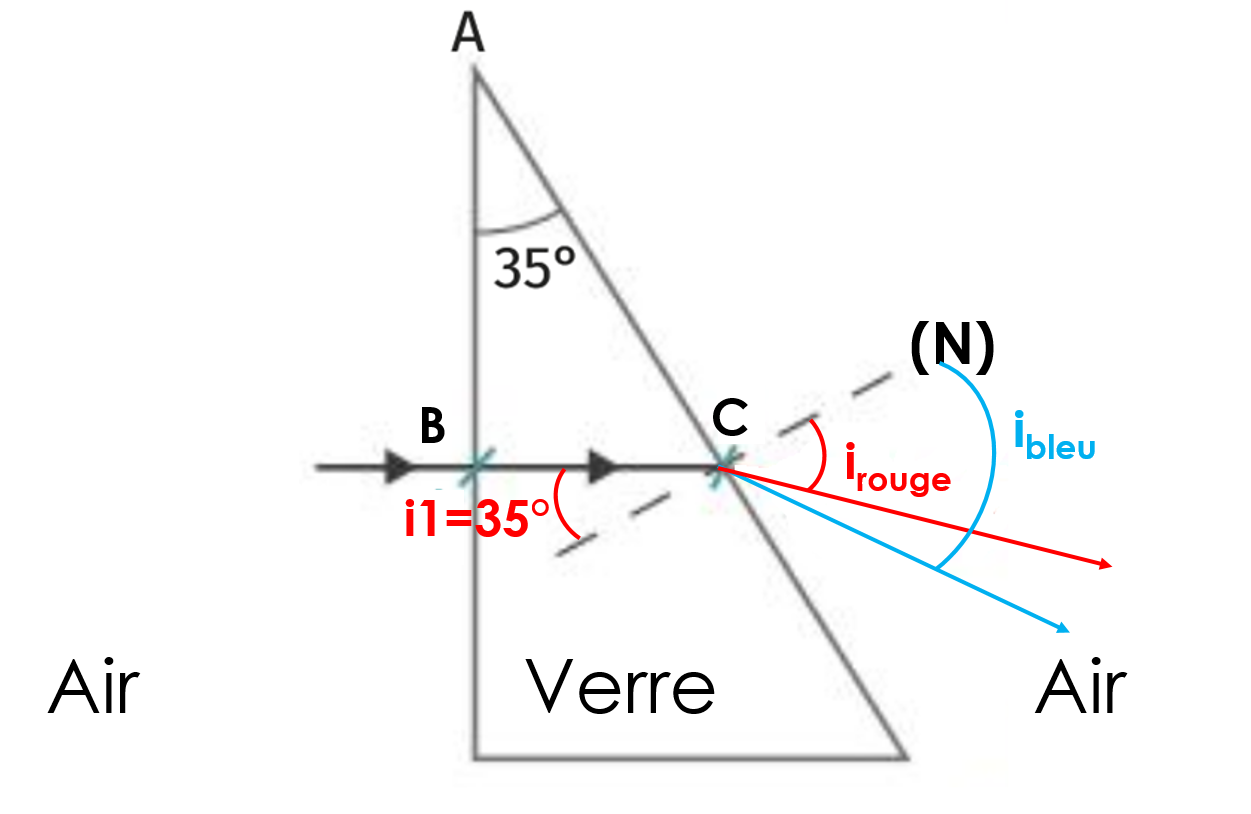
\includegraphics[scale=0.6]{Images/Prisme_correction10.png}
\end{center}}{0}
\end{difficile}
\hfill
%\end{minipage}

%\newpage

\begin{difficile}{\large Bilan de l'activité sur la dispersion}
\vspace{0.5cm}
\question{Quel phénomène permet d'expliquer la déviation de la lumière par le prisme ?}{Il s'agit de la réfraction. Celle-ci dépend de la longueur d'onde (la couleur autrement dit) de la lumière. Lorsque l'indice optique d'un milieu dépend de la longueur d'onde, on dit que le milieu est \underline{dispersif}.}{0}
\\
\question{Lors de la formation d'un arc-en-ciel, quel élément joue le rôle de prisme ?}{Il s'agit des gouttes d'eau composant la pluie.}{0}
    \texteTrouMultiLignes{~}{15}
\end{difficile}
%\newpage
%\papiermillimetre
  %%\modeCorrection

%%%% début de la page
\renewcommand{\thesection}{\textcolor{red}{Partie \Roman{section} -}}
\renewcommand{\thesubsection}{\textcolor{red}{\Roman{section}.\arabic{subsection}}}
\renewcommand{\thesubsubsection}{\textcolor{red}{\Roman{section}.\arabic{subsection}.\alph{subsubsection}}}

\setcounter{section}{0}
\setcounter{document}{0}
\sndEnTeteTPOnze

\begin{center}
\begin{mdframed}[style=titr, leftmargin=60pt, rightmargin=60pt, innertopmargin=7pt, innerbottommargin=7pt, innerrightmargin=8pt, innerleftmargin=8pt]

\begin{center}
\large{\textbf{TP 11 : L'\oe il, un instrument remarquable
}}
\end{center}
\end{mdframed}
\end{center}


%%%% objectifs
\begin{tcolorbox}[colback=blue!5!white,colframe=blue!75!black,title=Objectifs de la séance :]
\begin{itemize}
    \item Modéliser l'\oe il ;
    \item Produire et caractériser l'image réelle d'un objet plan réel formée par une lentille mince convergente ;
    \item Utiliser le théorème de Thalès ;
\end{itemize}
\end{tcolorbox}

%%%% Consignes
\begin{tcolorbox}[colback=red!5!white,colframe=red!75!black,title= Consignes :]
\begin{itemize}
    \item Faire attention au matériel lors de son utilisation ;
\end{itemize}
\end{tcolorbox}

%%%% contexte
\section{Analyse documentaire}
\begin{tcolorbox}[colback=orange!5!white,colframe=orange!75!black,title= C'est pas sorcier l'\oe il ! :]
Regarder la vidéo tirée de l'émission \og C'est pas Sorcier \fg~ à l'adresse suivante \url{https://ladigitale.dev/digiview/#/v/6576d364e2055} ou en scannant le QR-code : 
\begin{center}
    
\includegraphics[scale=0.4]{Images/CPasSorcier_Oeil.png}
\end{center}
Compléter le tableau suivant :
\begin{center}
    \begin{tabular}{|C{0.3}|C{0.3}|C{0.3}|}
    \hline
        \cellcolor{orange!25} \oe il & \cellcolor{orange!25} appareil photo & \cellcolor{orange!25} rôle \\
        \hline
        Cornée & %Lentille  
        & %Faire converger la lumière dans l'\oe il 
        \\
        \hline
        Iris & %Diaphragme 
        & %Faire passer plus ou moins de lumière dans l'\oe il 
        \\
        \hline 
        Cristallin & %Lentille 
        &%Faire converger la lumière sur la rétine
        \\
        \hline 
        Rétine & %Pélicule
        & %Reçoit la lumière/ Convertir le signal lumineux en signal électrique pour le cerveau 
        \\
        \hline 
    \end{tabular}
\end{center}

\problematique{Comment se propage la lumière à travers une lentille ? Quelle dimension a l'image d'un objet réel à travers une lentille convergente ?}
\end{tcolorbox}


\begin{mdframed}[style=autreexo]
\textbf{\bsc{Liste du matériel}}
\vspace{-0.5cm}
\begin{multicols}{2}
\begin{itemize}
    \item Une \og laser box \fg ;
    \item Des lentilles convergentes ;
    \item Un tableau magnétique ;
\end{itemize}
\end{multicols}
\end{mdframed}

%%%% documents

%%%%
\section{Propriétés des lentilles convergentes}

\subsection{Mise en évidence de 3 points particuliers}

\question{Observer sur le tableau magnétique le cheminement d'un rayon lumineux passant par le \textbf{centre de la lentille} aussi appelé \textcolor{red}{centre optique} et noté O.\\

\textit{Observations :} \texteTrouMultiLignes{Lorsqu'un rayon lumineux passe par le centre optique de la lentille, il \underline{n'est pas dévié}.}{1}
\begin{center}
    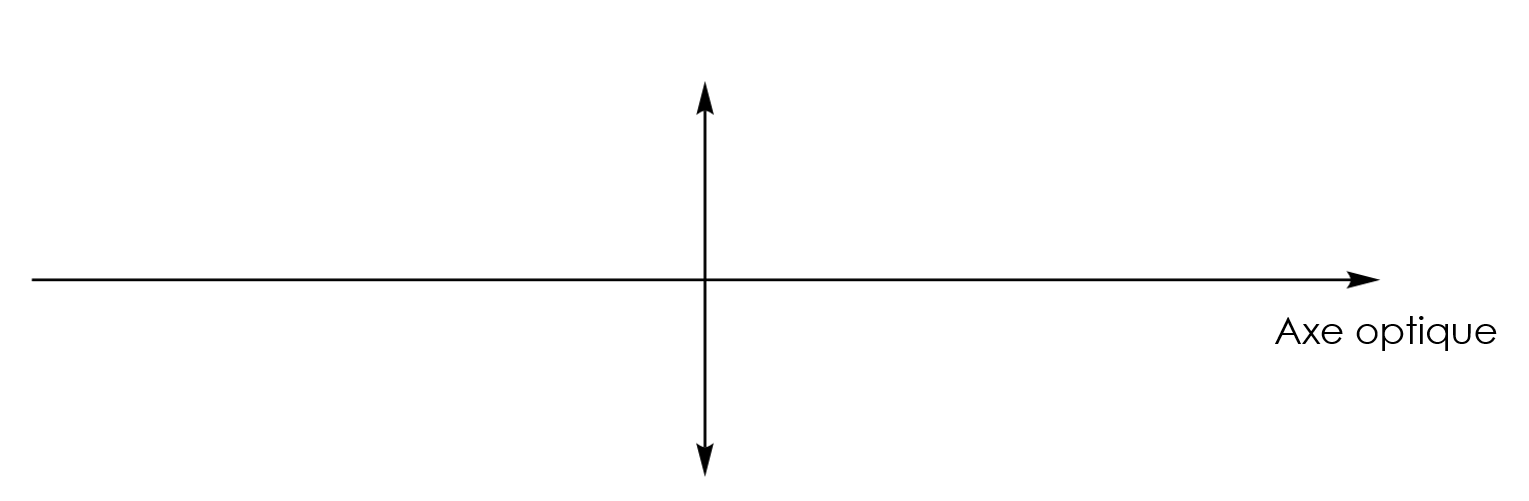
\includegraphics[scale=0.6]{Images/Lentille_construction.PNG}
\end{center}
}{\begin{center}
    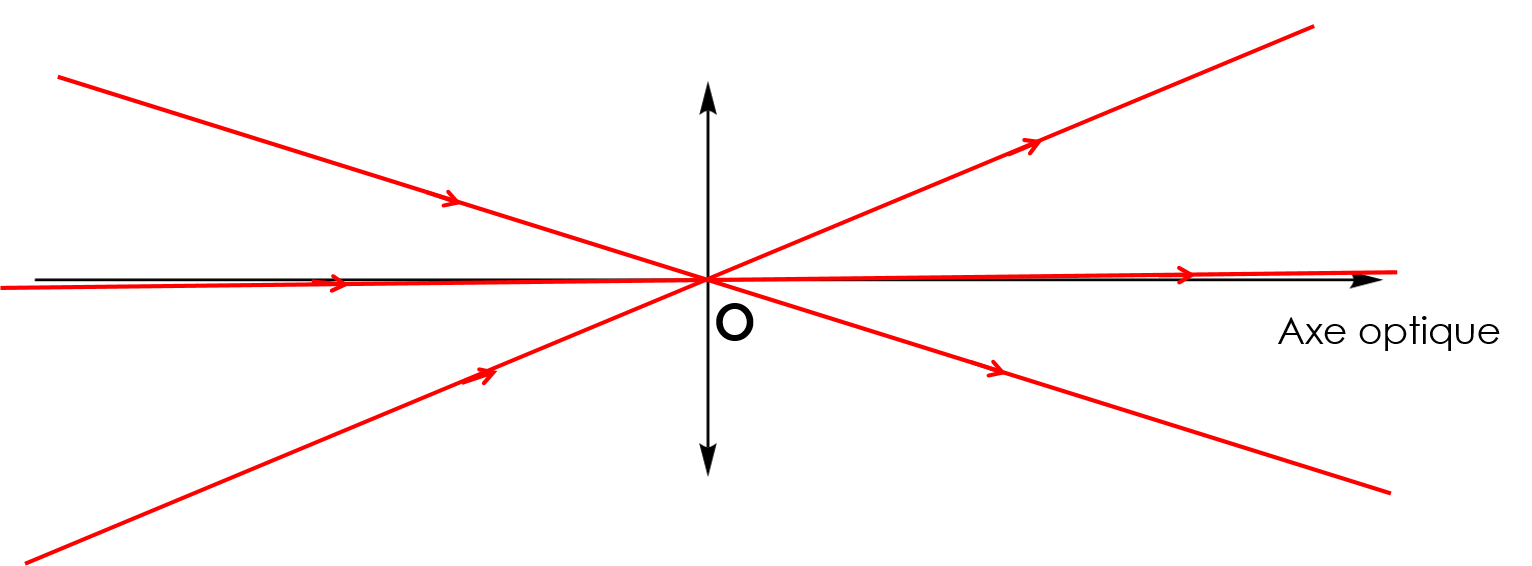
\includegraphics[scale=0.5]{Images/Lentille_construction_centreoptique.png}
\end{center}}{0}

\question{Observer sur le tableau magnétique le cheminement de rayons lumineux \textbf{arrivant parallèles à l'axe optique}.\\

\textit{Observations :} \texteTrouMultiLignes{Lorsqu'un rayon lumineux arrive parallèlement à l'axe optique, il ressort sur un point particulier appelé  \underline{foyer focal image}, noté F'.}{1}
\begin{center}
    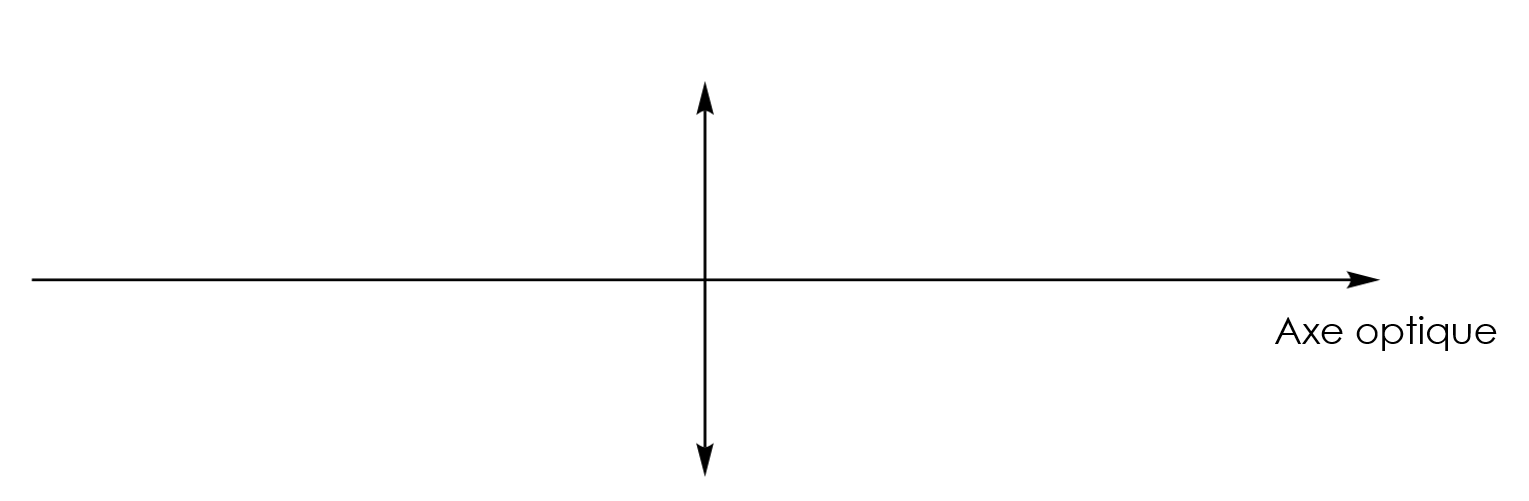
\includegraphics[scale=0.6]{Images/Lentille_construction.PNG}
\end{center}
}{\begin{center}
    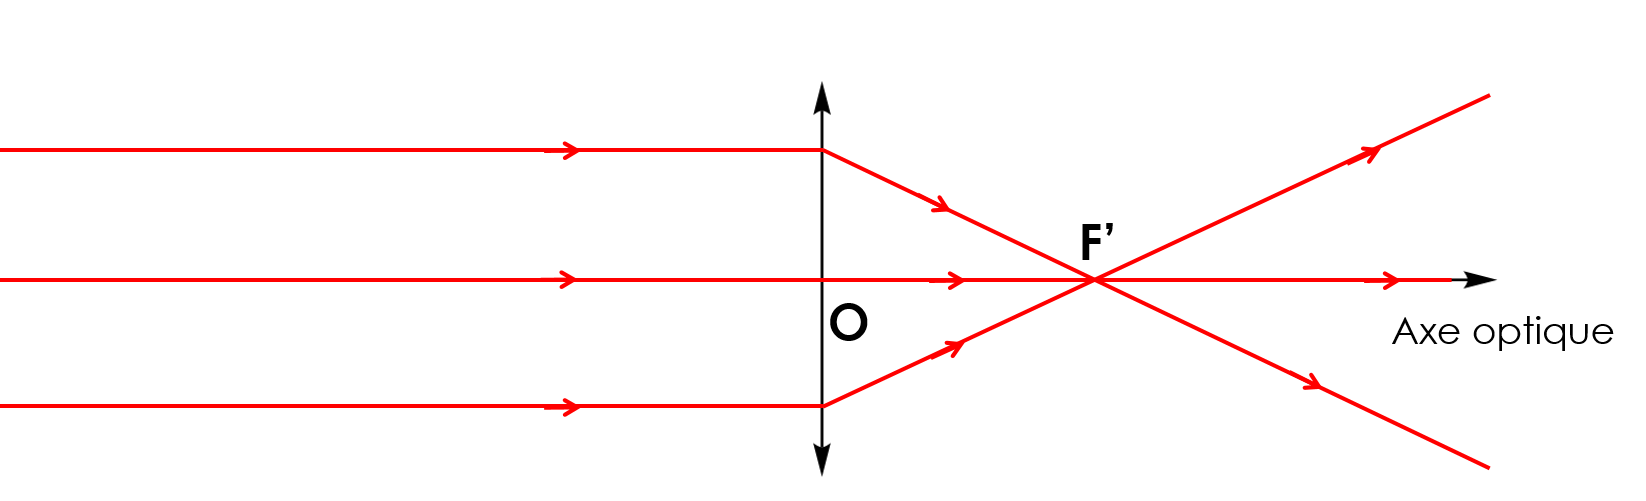
\includegraphics[scale=0.5]{Images/Lentille_construction_foyerimage.png}
\end{center}}{0}

\question{Observer sur le tableau magnétique le cheminement de rayons lumineux \textbf{émergeant parallèles à l'axe optique}.\\

\textit{Observations :} \texteTrouMultiLignes{Lorsqu'un rayon lumineux émerge parallèle à l'axe optique, il provient d'un point particulier appelé \underline{foyer focal objet}, noté F.}{2}
\begin{center}
    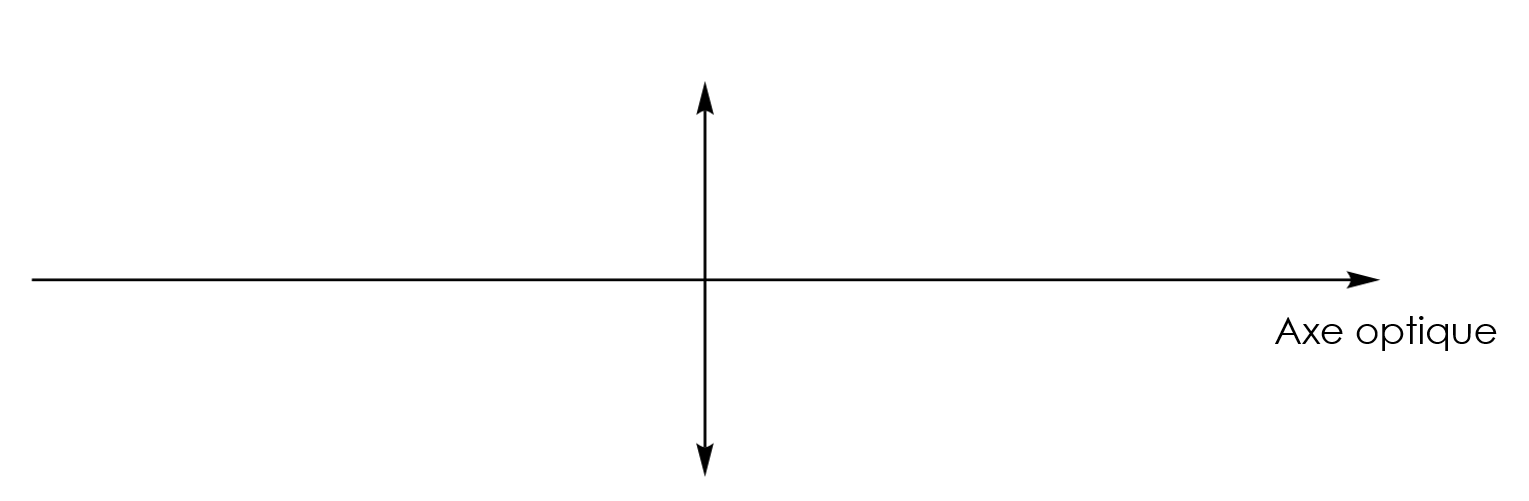
\includegraphics[scale=0.6]{Images/Lentille_construction.PNG}
\end{center}
}{\begin{center}
    \includegraphics[scale=0.5]{Images/Lentille_construction_foyerobjet.png}
\end{center}}{0}

\subsection{\`{A} retenir}

\begin{multicols}{2}
\begin{tcolorbox}[colback=green!5!white,colframe=green!75!black,title=\textbf{Lentille convergente :}]  
    Une lentille est caractérisée par son \textcolor{red}{centre optique} O par lequel passe l'axe optique, son \textcolor{red}{foyer image} F' et \textcolor{red}{son foyer objet} F.
\end{tcolorbox}
\begin{tcolorbox}[colback=red!5!white,colframe=red!75!black,title=\textbf{Propriété sur F et F' :}]
Les foyers objets F et images F' sont \textcolor{red}{symétriques} par rapport au centre optique O de la lentille.
\end{tcolorbox}

\end{multicols}
    \begin{tcolorbox}[colback=red!5!white,colframe=red!75!black,title=\textbf{Règles de construction d'une image par une lentille :}]
\begin{itemize}
    \item Le rayon passant par le centre optique O \textbf{n'est pas dévié} ;
    \item Les rayons arrivant parallèlement à l'axe optique \textbf{ressortent sur le foyer image F'} ;
    \item Les rayons passant par le foyer objet F \textbf{ressortent parallèle à l'axe optique $\Delta$}.
\end{itemize}
\end{tcolorbox}
\newpage
\section{Image d'un objet plan à travers une lentille convergente}
\setcounter{exercice}{0}

\begin{mdframed}[style=autreexo]
\textbf{\bsc{Liste du matériel}}
\vspace{-0.5cm}
\begin{multicols}{2}
\begin{itemize}
    \item Une source de lumière avec un objet plan ;
    \item Une lentille convergentes de distance focale OF'=f'=12,5~cm (8 dioptries) ;
    \item Un banc optique ;
    \item Un écran recouvert d'un papier millimétré;
\end{itemize}
\end{multicols}
\end{mdframed}

\begin{doc}{Protocole expérimental}
\begin{center}
    \includegraphics[scale=0.7]{Images/Protocole_lentille.PNG}
\end{center}
   \begin{enumerate}
       \item Réaliser le montage ci-dessus ;
       \item Mesurer la taille de l'objet lumineux AB ;
       \item Placer la lentille convergente à différentes distances de l'objet lumineux et mesurer la distance entre l'objet et la lentille OA à l'aide du banc optique ;
       \item Déplacer l’écran pour observer une \textbf{image nette} sur l’écran ;
       \item Mesurer la distance entre la lentille et l'écran notée $\overline{\text{OA'}}$ ;
       \item Mesurer la taille $\overline{\text{A'B'}}$ de l'image sur l'écran ;
   \end{enumerate}
\end{doc}

\begin{tcolorbox}[colback=green!5!white,colframe=green!75!black,title=\textbf{Définition du grandissement :}]  
    On appelle \textcolor{red}{grandissement}, noté $\gamma$, le rapport entre la taille \textcolor{red}{algébrique} de l'image $\overline{\text{A'B'}}$ et celle de l'objet $\overline{\text{AB}}$ :
    \begin{equation*}
        \gamma = \frac{\overline{\text{A'B'}}}{\overline{\text{AB}}}
    \end{equation*}
    \begin{itemize}
    \item Si $\gamma$ est négatif, alors l'image est renversée ;
    \item Si $\abs{\gamma}$ est plus petit que 1, alors l'image est plus petite que l'objet.
\end{itemize}
\end{tcolorbox}
\clearpage
%\vspace{-0.5cm}
\question{Mettre en \oe uvre les \textbf{4 premières étapes} protocole expérimental donné dans le document 1 en prenant $\overline{\text{OA}}$ = -30~cm.}{On mesure AB=5cm.}{0}
%\\
\question{Indiquer si l'image est droite ou renversée, agrandie ou rétrécie.}{L'image est renversée et rétrécie.}{0}
%\\
%\clearpage
\question{Compléter le schéma suivant en plaçant l'axe optique, le centre optique O, le foyer focal objet F et le foyer focal image F'. \`{A} l'aide des règes de construction énoncées dans la partie II, tracer les rayons lumineux provenant de B pour construire l'image B' à travers la lentille. 
\begin{center}
    \includegraphics[scale=0.9]{Images/Lentille_construction_papier.png}
\end{center}}{\begin{center}
    \includegraphics[scale=0.6]{Images/Lentille_construction_papier_correction.png}
\end{center}}{0}
\newpage
\question{Réaliser le protocole du document 1 et compléter le tableau suivant : 
\begin{center}
    \begin{tabular}{|C{0.2}|C{0.15}|C{0.15}|C{0.15}|C{0.15}| }
        \hline 
        \cellcolor{orange!25} Expérience & \cellcolor{blue!25}n$\degree$1 & \cellcolor{blue!25}n$\degree$2 & \cellcolor{blue!25}n$\degree$3 & \cellcolor{blue!25}n$\degree$4\\
         \hline
         \cellcolor{orange!25} Distance $\overline{\text{OA}}$ (en cm) & -15 & -30 & -50 & -60 \\
         \hline
         \cellcolor{orange!25} Distance $\overline{\text{OA'}}$ (en cm) & & & &  \\
         \hline
         \cellcolor{orange!25} Nature de l'image (agrandie ou rétrécie, droite ou renversée) & & & & \\
         \hline
         \cellcolor{orange!25} Taille de l'image $\overline{\text{AB'}}$ (en cm) & & & & \\
         \hline
    \end{tabular}
\end{center}}{\begin{center}
    \begin{tabular}{|C{0.2}|C{0.15}|C{0.15}|C{0.15}|C{0.15}| }
        \hline 
        \cellcolor{orange!25} Expérience & \cellcolor{blue!25}n$\degree$1 & \cellcolor{blue!25}n$\degree$2 & \cellcolor{blue!25}n$\degree$3 & \cellcolor{blue!25}n$\degree$4\\
         \hline
         \cellcolor{orange!25} Distance $\overline{\text{OA}}$ (en cm) & -15 & -30 & -50 & -60 \\
         \hline
         \cellcolor{orange!25} Distance $\overline{\text{OA'}}$ (en cm) & 75 & 21 & 17 & 16 \\
         \hline
         \cellcolor{orange!25} Nature de l'image (agrandie ou rétrécie, droite ou renversée) & Agrandie, renversée & Rétrécie, renversée & Rétrécie, renversée & Rétrécie, renversée\\
         \hline
         \cellcolor{orange!25} Taille de l'image $\overline{\text{AB'}}$ (en cm) & -25 & -3,5 & -1,7 & -1,3 \\
         \hline
    \end{tabular}
\end{center}}{0}

\question{Indiquer comment varie la taille de l'image lorsqu'on rapproche l'objet de la lentille.}{La taille de l'image augmente. On ne peut même plus obtenir d'image nette à partir si OA<12,5cm.}{0}

\question{\`{A} l'aide de vos résultats dans le tableau précédent, compléter le tableau suivant :
\begin{center}
    \begin{tabular}{|C{0.2}|C{0.15}|C{0.15}|C{0.15}|C{0.15}| }
        \hline 
        \cellcolor{orange!25} Expérience & \cellcolor{blue!25}n$\degree$1 & \cellcolor{blue!25}n$\degree$2 & \cellcolor{blue!25}n$\degree$3 & \cellcolor{blue!25}n$\degree$4\\
        \hline
        \cellcolor{orange!25} $\frac{\overline{\text{OA'}}}{\overline{\text{OA}}}$ & & & &  \\
        \hline
        \cellcolor{orange!25} Grandissement $\gamma$ &  &  &  & \\
        \hline 
    \end{tabular}
\end{center}
}{\begin{center}
    \begin{tabular}{|C{0.2}|C{0.15}|C{0.15}|C{0.15}|C{0.15}| }
        \hline 
        \cellcolor{orange!25} Expérience & \cellcolor{blue!25}n$\degree$1 & \cellcolor{blue!25}n$\degree$2 & \cellcolor{blue!25}n$\degree$3 & \cellcolor{blue!25}n$\degree$4\\
        \hline
        \cellcolor{orange!25} $\frac{\overline{\text{OA'}}}{\overline{\text{OA}}}$ & -5 & -0,7 & -0,34 & -0,27 \\
        \hline
        \cellcolor{orange!25} Grandissement $\gamma$ & -5 & -0,7 & -0,34 & -0,27\\
        \hline 
    \end{tabular}
\end{center}}{0}

\question{Proposer une relation entre le grandissement et le rapport $\frac{\overline{\text{OA'}}}{\overline{\text{OA}}}$.}{D'après les mesures expérimentales, on peut conjecturer que $\gamma=\frac{\overline{\text{OA'}}}{\overline{\text{OA}}}$}{0}

\question{\`{A} l'aide du théorème de Thalès dans les triangles OAB et OA'B' (voir la question 6), démontrer la relation conjecturée dans la question précédente.}{Dans les triangles OAB et OA'B', les droites (AB) et (A'B') sont parallèles. On peut dès lors appliquer le théorème de Thalès qui donne les relations suivantes :
\begin{equation*}
    \frac{\overline{\text{OA'}}}{\overline{\text{OA}}} = \frac{\overline{\text{A'B'}}}{\overline{\text{AB}}} = \frac{\overline{\text{OB'}}}{\overline{\text{OB}}}
\end{equation*}
La première égalité donne la relation recherchée.}{0}
%\\

\begin{facile}{\large Simulation sur les lentilles}
\vspace{0.5cm}
\begin{multicols}{2}
\begin{center}
    On aurait pu tout faire à l'aide de ce logiciel de simulation (merci l'université du Colorado !) :

    \url{https://phet.colorado.edu/fr/simulations/geometric-optics-basics}\\
    \vspace{4cm}
    \begin{Large}
        \textbf{Mais c'est quand même bien mieux d'expérimenter en TP, non ??}
    \end{Large}
\end{center}

%\begin{center}
 %   \includegraphics[scale=0.15]{Images/Joyeux_noel_dispersé.png}
%\end{center}
\end{multicols}


\end{facile}
%\newpage
%\papiermillimetre
  

  %%%%%%%%%% Devoirs Notés %%%%%%%%%%
  %%\modeCorrection


\renewcommand{\thesubsection}{\textcolor{red}{\Roman{section}.\arabic{subsection}}}
\renewcommand{\thesubsubsection}{\textcolor{red}{\Roman{section}.\arabic{subsection}.\alph{subsubsection}}}
\renewcommand{\titreDocu}[1]{
  \refstepcounter{document} % update counter
  \textbf{Exercice \arabic{document} -- #1} 
  \addcontentsline{toc}{document}{\protect\numberline{} #1} % update table of content
}

\setcounter{section}{0}
\setcounter{document}{0}


\nomPrenomClasse
\vspace{1cm}

\begin{center}
\begin{mdframed}[style=titr, leftmargin=60pt, rightmargin=60pt, innertopmargin=7pt, innerbottommargin=7pt, innerrightmargin=8pt, innerleftmargin=8pt]
\begin{center}
\begin{Large}
    Devoir Surveillé n°3 (sujet A) : Propagation de la lumière dans les milieux (55min)
\end{Large}
\end{center}
\end{mdframed}
\end{center}
\vspace{1cm}

\begin{tableauCompetences}
    APP & Connaître les définitions du cours & & & & \\
    \hline
    REA & Réaliser ou compléter un schéma & & & & \\
\hline
    ANA &  Exploiter des informations extraites des données & & & & 
\end{tableauCompetences}

\begin{tcolorbox}[colback=red!5!white,colframe=red!75!black,title=\textbf{Consignes : }]
   \begin{enumerate}
        \item Vous rédigerez tout sur le sujet,
        \item Pour les élèves bénéficiant d'un PAP, vous ne traiterez pas les questions marquées par $(*)$ ; 
        %\item La calculatrice \underline{n'est pas autorisée}.
   \end{enumerate}
\end{tcolorbox}

\begin{doc}{Quizz \begin{Large}
    /4 points
\end{Large}}
Entourer \underline{la} bonne réponse :
\begin{enumerate}
    \item \textbf{La lumière se propage dans le vide à la vitesse (1pt):}
        \begin{align*}
            a.& ~\text{$c=3\times10^8$~km$\cdot$h$^{-1}$} & b.& ~\text{$c=3\times10^8$~m$\cdot$s$^{-1}$} & c.& ~\text{$c=340$~m$\cdot$s$^{-1}$ à la température T=15$\degreCelsius$}
            %a.& ~\text{$c=3\times10^8$~km$\cdot$h$^{-1}$} & b.& ~\text{\textcolor{red}{$c=3\times10^8$~m$\cdot$s$^{-1}$}} & c.& ~\text{$c=340$~m$\cdot$s$^{-1}$ à la température T=15$\degreCelsius$}
        \end{align*}
    \item \textbf{$(*)$La normale au dioptre est (1pt):}
        \begin{align*}
            a.& ~\text{un objet qui permet de disperser la lumière} & b.&~\text{une ligne imaginaire perpendiculaire à l'interface} \\
            c.& ~\text{l'interface entre deux milieux différents} & d.&~\text{un instrument de musique}
            %a.& ~\text{un objet qui permet de disperser la lumière} & b.&~\text{\textcolor{red}{une ligne imaginaire perpendiculaire à l'interface}} \\
            %c.& ~\text{l'interface entre deux milieux différents} & d.&~\text{un instrument de musique}
        \end{align*}
    %\item (*)\textbf{Un rayon lumineux passant par la normale (1pt): }
    %    \begin{align*}
    %        a.& ~\text{le rayon n'est pas dévié à l'interface} & b.& ~\text{il y a réfraction à l'interface} \\
    %        c.& ~\text{Le rayon s'éloigne de la normale} & d.& ~\text{le rayon se rapproche de la normale}
            %a.& ~\text{le rayon n'est pas dévié à l'interface} & b.& ~\text{\textcolor{red}{il y a réfraction à l'interface} } \\
            %c.& ~\text{Le rayon s'éloigne de la normale} & d.& ~\text{\textcolor{red}{le rayon se rapproche de la normale}} 
    %    \end{align*}
    \item \textbf{L'indice optique d'un milieu est (1pt):}
        \begin{align*}
            a.& ~\text{plus petit que 1} & b.& ~\text{plus grand que 1} & c.& ~\text{égal à 1 dans le plexiglas} 
            %a.& ~\text{plus petit que 1} & b.& ~\text{\textcolor{red}{plus grand que 1}} & c.& ~\text{égal à 1 dans le plexiglas} 
        \end{align*}
    \item \textbf{Le cristallin de l'\oe il (1pt):}
    \begin{align*}
            a.& ~\text{se modélise par une lentille convergente} & b.~\text{est fait en cristal} \\
            c.& ~\text{convertit un signal lumineux en signal électrique} 
            %a.& ~\text{\textcolor{red}{se modélise par une lentille convergente}} & b.& ~\text{est fait en cristal} \\
            %c.& ~\text{convertit un signal lumineux en signal électrique} 
        \end{align*}
\end{enumerate}
\end{doc}

\begin{doc}{L'objectif d'un microscope \begin{Large}
    /8 points
\end{Large}}
%\begin{wrapfigure}{r}{0.2\textwidth}
\begin{center}
    \includegraphics[scale=0.4]{Images/Microscope.png}
\end{center}
      
 % \end{wrapfigure}
L'image de droite ci-dessus représente l'image d'une patte de Gecko embryonnaire obtenue à l'aide d'une technique de microscopie très particulière appelée \og confocale \fg. Cette image a remporté le prestigieux concours d'imagerie de microscopie en 2022 organisé chaque année par la marque Nikon.\\
Un microscope sert à rendre visible pour l'\oe il des objets de taille microscopique (jusqu'au dixième de nanomètre pour les meilleurs microscopes !). \\
Un microscope standard est constitué d'un oculaire et d'un ou de plusieurs objectifs (voir la figure de gauche ci-dessus) qui sont tous les deux des lentilles convergentes. On se propose ici d'évaluer le grandissement d'une lentille convergente.

\question{Compléter le schéma ci-dessous avec les informations suivantes : centre optique \textbf{O}, \textbf{axe optique}, foyer focal objet \textbf{F}, foyer focal image \textbf{F'}. (2pts)
\begin{center}
\includegraphics[scale=0.45]{Images/Construction_lentille_SujetA.png}    
\end{center}}{\begin{center}
\includegraphics[scale=0.45]{Images/Construction_lentille_SujetA_correction1.png}    
\end{center}}{0}

%\vspace{-5pt}
\question{\`{A} l'aide d'au moins deux rayons lumineux, construire sur le schéma précédent l'image A'B' de AB à travers la lentille. (2pts)}{\begin{center}
\includegraphics[scale=0.45]{Images/Construction_lentille_SujetA_correction2.png}    
\end{center}}{0}

\question{Caractériser l'image obtenue (agrandie, rétrécie, renversée, droite) et en déduire le signe du grandissement $\gamma$. (2pts)\newline
\texteTrouMultiLignes{~}{2}}{L'image est ici rétrécie et renversée. Comme l'image est renversée $\gamma<0$.}{0}
%\\
\question{\`{A} l'aide de votre schéma, déterminer la valeur absolue du grandissement $\abs{\gamma}$ (rappel : $\abs{\gamma}>0$) de cette lentille. (1pt)\newline
\texteTrouMultiLignes{~}{2}}{Par lecture graphique (ou avec une règle mais ici le calcul est simple), on a :
\begin{equation*}
    \abs{\gamma} = \frac{\text{A'B'}}{\text{AB}} =\frac{2\text{ carreaux}}{4 \text{ carreaux}} = 0,5
\end{equation*}}{0}
%\\
\question{$(*)$Cette valeur est-elle cohérente avec votre schéma ? Justifier. (1pt)\newline
\texteTrouMultiLignes{~}{2}}{Oui cette valeur est cohérente car l'image est rétrécie et $\abs{\gamma}<1$.}{0}
%\\

%\question{$(*)$Sachant qu'il existe un oculaire et un objectif sur un microscope, l'image est-elle droite ou renversée à la sortie d'un microscope. Justifier.(1pt)\newline
%\texteTrouMultiLignes{~}{3}}{L'image à travers une lentille convergente est à chaque fois renversée par rapport à l'objet. Comme l'objet pour l'oculaire est A'B', son image (qu'on peut appeler A"B" par exemple) sera renversée par rapport à A'B'. Elle sera donc dans le même sens que l'objet AB.}{0}
\end{doc}
\clearpage
\begin{doc}{Les essuies-glace automatiques \begin{Large}
    /8 points
\end{Large}}
\setcounter{exercice}{0}
%\begin{wrapfigure}{r}{0.2\textwidth}
\begin{minipage}{0.5\textwidth}
\begin{center}
    \includegraphics[scale=0.55]{Images/Essuis_glace.png}
\end{center}
\end{minipage}
\begin{minipage}{0.5\textwidth}
\begin{center}
    \includegraphics[scale=0.45]{Images/Temps_sec.PNG}
\end{center}
\end{minipage}
Un essuie-glace automatique se met en marche lorsqu'il y a des gouttes de pluie sur le pare-brise. Le schéma ci-dessus illustre le principe de détection d'un faisceau laser envoyé dans un pare-brise (conçu en verre feuilleté) par temps sec : la lumière du laser envoyé par l'émetteur reste confiné dans le pare-brise et arrive jusqu'à un récepteur.\vspace{1cm}%\clearpage

\question{Identifier le phénomène (réflexion, réfraction, dispersion) qui permet au laser de rester confiné dans le pare-brise. (1pt) \newline \texteTrouMultiLignes{~}{1}}{Il s'agit du phénomène de réflexion de la lumière.}{0}
%\\

Lorsque la pluie tombe sur le pare-brise, les gouttes d'eau permettent de laisser passer la lumière du laser à l'interface verre-eau. \\
\question{Identifier le phénomène (réflexion, réfraction, dispersion) qui explique la propagation de la lumière du pare-brise vers la goutte d'eau. (1pt)\newline \texteTrouMultiLignes{~}{1}}{Il s'agit du phénomène de réfraction.}{0}

\vspace{2cm}
Sur la figure de la page suivante, on a réalisé une modélisation de l'interface entre l'essuie-glace (le verre donc) et la goutte d'eau.%\clearpage
\begin{center}
\includegraphics[scale=0.45]{Images/Interface.PNG}    
\end{center}
L'émetteur envoie un rayon lumineux arrivant avec un angle d'incidence $i_1=30\degree$ à cette interface. On donne $n_{\text{eau}}=1,33$ et $n_{\text{verre}}=1,47$.\\
\question{Compléter le schéma en faisant apparaître la normale au dioptre, les indices $n_{verre}$ et $n_{eau}$, les rayons incident et réfracté ainsi que le sens de propagation de la lumière, leurs angles associés notés $i_1$ et $i_2$. (2pts)
}{\begin{center}
    \includegraphics[scale=0.45]{Images/Interface_corriger.png}
\end{center}}{0}

\question{\'{E}noncer la 2$^{\text{ème}}$ loi de Snell-Descartes sur la réfraction. (1pt)\newline
\texteTrouMultiLignes{}{2}}{Le rayon incident, réfracté appartiennent au même plan appelé \textcolor{red}{plan d'incidence}.\\
L'angle d'incidence $i_1$ et l'angle de réfraction $i_2$ sont reliés par la formule suivante :
\begin{empheq}[box=\fbox]{equation*}
    n_1 \sin\left(i_1\right)= n_2 \sin\left(i_2\right)
\end{empheq}}{0}

\question{$(*)$Calculer l'angle de réfraction $i_2$. (2pts)\newline
\texteTrouMultiLignes{~}{3}}{On a d'après la formule précédente : 
\begin{align*}
    n_{\text{verre}} \sin\left(i_1\right)&= n_{\text{eau}} \sin\left(i_2\right) \\
    \text{donc~}\sin\left(i_2\right) &= \frac{n_{\text{verre}}}{n_{\text{eau}}}\sin\left(i_1\right) \\
    \text{donc~} i_2 &= \arcsin\left(\frac{n_{\text{verre}}}{n_{\text{eau}}}\sin\left(i_1\right)\right) = \arcsin\left(\frac{1,47}{1,33}\sin\left(30\degree\right)\right) = 33,5\degree
\end{align*}
La valeur est cohérente car on passe d'un milieu moins réfringeant à un milieu plus réfringeant.}{0}
%\\
Lorsque le récepteur ne reçoit plus 100\% de la lumière émise, les essuies-glace se mettent en marche.\\
\question{$(*)$Expliquer pourquoi les essuies-glace se mettent en route par temps de pluie. (1pt)\newline
\texteTrouMultiLignes{}{3}}{A chaque passage de la lumière à l'interface verre-eau, une partie de la lumière est réfracté et donc sort à l'extérieur du pare-brise. L'intensité diminue donc et le récepteur ne reçoit plus 100\% de la lumière émise déclanchant les essuie-glace.}{0}
%\\
\question{\textit{(Bonus)} Démontrer qu'à partir d'un certain angle d'incidence noté $i_{1,lim}$, il n'y a plus de réfraction. On appelle ce phénomène \textbf{\underline{la réflexion totale}}. (2pts)\newline
\texteTrouMultiLignes{}{4}}{Plus l'angle d'incidence augmente, plus l'angle de réfraction augmente d'après la loi de Descartes sur la réfraction. Comme $n_{verre}>n_{eau}$, $i_1<i_2$. Or comme les angles ne peuvent prendre que des valeurs entre 0 et 90$\degree$, il existe un angle $i_{i,lim}$ à partir duquel $i_{2}=90\degree$. Au-delà de cet angle d'incidence, il n'existe plus de rayon réfracté et toute l'intensité de la lumière est réfléchie dans le pare-brise.}{0}
\end{doc}

\begin{facile}{Bonus de relecture (+0,5pt)}
    Relisez vos réponses et évaluez votre copie sur 20. \\
    \begin{center}
        Selon moi, je pense avoir ...../20
    \end{center}
    Si la différence entre votre note réelle est celle que vous évaluez est supérieure à 2 points, le bonus ne comptera pas.
\end{facile}
  %\modeCorrection


\renewcommand{\thesubsection}{\textcolor{red}{\Roman{section}.\arabic{subsection}}}
\renewcommand{\thesubsubsection}{\textcolor{red}{\Roman{section}.\arabic{subsection}.\alph{subsubsection}}}
\renewcommand{\titreDocu}[1]{
  \refstepcounter{document} % update counter
  \textbf{Exercice \arabic{document} -- #1} 
  \addcontentsline{toc}{document}{\protect\numberline{} #1} % update table of content
}

\setcounter{section}{0}
\setcounter{document}{0}


\nomPrenomClasse
\vspace{1cm}

\begin{center}
\begin{mdframed}[style=titr, leftmargin=60pt, rightmargin=60pt, innertopmargin=7pt, innerbottommargin=7pt, innerrightmargin=8pt, innerleftmargin=8pt]
\begin{center}
\begin{Large}
    Devoir Surveillé n°3 (sujet B) : Propagation de la lumière dans les milieux (55min)
\end{Large}
\end{center}
\end{mdframed}
\end{center}
\vspace{1cm}

\begin{tableauCompetences}
    APP & Connaître les définitions du cours & & & & \\
    \hline
    REA & Réaliser ou compléter un schéma & & & & \\
\hline
    ANA &  Exploiter des informations extraites des données & & & & 
\end{tableauCompetences}

\begin{tcolorbox}[colback=red!5!white,colframe=red!75!black,title=\textbf{Consignes : }]
   \begin{enumerate}
        \item Vous rédigerez tout sur le sujet,
        \item Pour les élèves bénéficiant d'un PAP, vous ne traiterez pas les questions marquées par $(*)$ ; 
        %\item La calculatrice \underline{n'est pas autorisée}.
   \end{enumerate}
\end{tcolorbox}

\begin{doc}{Quizz \begin{Large}
    /4 points
\end{Large}}
Entourer \underline{la} bonne réponse :
\begin{enumerate}
    \item \textbf{L'indice optique d'un milieu est (1pt):}
        \begin{align*}
            a.& ~\text{plus petit que 1} & b.& ~\text{plus grand que 1} & c.& ~\text{égal à 1 dans le plexiglas} 
            %a.& ~\text{plus petit que 1} & b.& ~\text{\textcolor{red}{plus grand que 1}} & c.& ~\text{égal à 1 dans le plexiglas} 
        \end{align*}
    \item \textbf{$(*)$Une normale au dioptre est (1pt):}
        \begin{align*}
            a.& ~\text{un objet qui permet de disperser la lumière} & b.&~\text{une ligne imaginaire perpendiculaire à l'interface} \\
            c.& ~\text{l'interface entre deux milieux différents} & d.&~\text{un instrument de musique}
            %a.& ~\text{un objet qui permet de disperser la lumière} & b.&~\text{\textcolor{red}{une ligne imaginaire perpendiculaire à l'interface}} \\
            %c.& ~\text{l'interface entre deux milieux différents} & d.&~\text{un instrument de musique}
        \end{align*}
    %\item (*)\textbf{Un rayon lumineux passant par la normale (1pt): }
    %    \begin{align*}
    %        a.& ~\text{le rayon n'est pas dévié à l'interface} & b.& ~\text{il y a réfraction à l'interface} \\
    %        c.& ~\text{Le rayon s'éloigne de la normale} & d.& ~\text{le rayon se rapproche de la normale}
            %a.& ~\text{le rayon n'est pas dévié à l'interface} & b.& ~\text{\textcolor{red}{il y a réfraction à l'interface} } \\
            %c.& ~\text{Le rayon s'éloigne de la normale} & d.& ~\text{\textcolor{red}{le rayon se rapproche de la normale}} 
    %    \end{align*}
    \item \textbf{La lumière se propage dans le vide à la vitesse (1pt):}
        \begin{align*}
            a.& ~\text{$c=3\times10^8$~km$\cdot$h$^{-1}$} & b.& ~\text{$c=3\times10^8$~m$\cdot$s$^{-1}$} & c.& ~\text{$c=340$~m$\cdot$s$^{-1}$ à la température T=15$\degreCelsius$}
            %a.& ~\text{$c=3\times10^8$~km$\cdot$h$^{-1}$} & b.& ~\text{\textcolor{red}{$c=3\times10^8$~m$\cdot$s$^{-1}$}} & c.& ~\text{$c=340$~m$\cdot$s$^{-1}$ à la température T=15$\degreCelsius$}
        \end{align*}
    \item \textbf{La rétine de l'\oe il (1pt):}
    \begin{align*}
            a.& ~\text{se modélise par une lentille convergente} & b.~\text{est fait en cristal} \\
            c.& ~\text{convertit un signal lumineux en signal électrique} 
            %a.& ~\text{se modélise par une lentille convergente} & b.& ~\text{est fait en cristal} \\
            %c.& ~\text{\textcolor{red}{convertit un signal lumineux en signal électrique}} 
        \end{align*}
\end{enumerate}
\end{doc}

\begin{doc}{L'objectif d'un microscope \begin{Large}
    /8 points
\end{Large}}
%\begin{wrapfigure}{r}{0.2\textwidth}
\begin{center}
    \includegraphics[scale=0.4]{Images/Microscope.png}
\end{center}
      
 % \end{wrapfigure}
L'image de droite ci-dessus représente l'image d'une patte de Gecko embryonnaire obtenue à l'aide d'une technique de microscopie très particulière appelée \og confocale \fg. Cette image a remporté le prestigieux concours d'imagerie de microscopie en 2022 organisé chaque année par la marque Nikon.\\
Un microscope sert à rendre visible pour l'\oe il des objets de taille microscopique (jusqu'au dixième de nanomètre pour les meilleurs microscopes !). \\
Un microscope standard est constitué d'un oculaire et d'un ou de plusieurs objectifs (voir la figure de gauche ci-dessus) qui sont tous les deux des lentilles convergentes. On se propose ici d'évaluer le grandissement d'une lentille convergente.

\question{Compléter le schéma ci-dessous avec les informations suivantes : centre optique \textbf{O}, \textbf{axe optique}, foyer focal objet \textbf{F}, foyer focal image \textbf{F'}. (2pts)
\begin{center}
\includegraphics[scale=0.45]{Images/Construction_lentille_SujetB.png}    
\end{center}}{\begin{center}
\includegraphics[scale=0.45]{Images/Construction_lentille_SujetB_correction1.png}    
\end{center}}{0}
%\\
%\vspace{-5pt}
\question{\`{A} l'aide d'au moins deux rayons lumineux, construire sur le schéma précédent l'image A'B' de AB à travers la lentille. (2pts)}{\begin{center}
\includegraphics[scale=0.45]{Images/Construction_lentille_SujetB_correction2.png}    
\end{center}}{0}

\question{Caractériser l'image obtenue (agrandie, rétrécie, renversée, droite) et en déduire le signe du grandissement $\gamma$. (2pts)\newline
\texteTrouMultiLignes{~}{2}}{L'image est ici agrandie et renversée. Comme l'image est renversée $\gamma<0$.}{0}
%\\
\question{\`{A} l'aide de votre schéma, déterminer la valeur absolue du grandissement $\abs{\gamma}$ (rappel : $\abs{\gamma}>0$) de cette lentille. (1pt)\newline
\texteTrouMultiLignes{~}{2}}{Par lecture graphique (ou avec une règle mais ici le calcul est simple), on a :
\begin{equation*}
    \abs{\gamma} = \frac{\text{A'B'}}{\text{AB}} =\frac{8\text{ carreaux}}{4 \text{ carreaux}} = 2
\end{equation*}}{0}
%\\
\question{$(*)$Cette valeur est-elle cohérente avec votre schéma ? Justifier. (1pt)\newline
\texteTrouMultiLignes{~}{2}}{Oui cette valeur est cohérente car l'image est agrandie et $\abs{\gamma}>1$.}{0}

%\vspace{-5pt}
%\question{$(*)$Sachant qu'il existe un oculaire et un objectif sur un microscope, expliquer pourquoi un observateur voit une image droite à travers le microscope. (1pt)\newline
%\texteTrouMultiLignes{~}{3}}{L'image à travers une lentille convergente est à chaque fois renversée par rapport à l'objet. Comme l'objet pour l'oculaire est A'B', son image (qu'on peut appeler A"B" par exemple) sera renversée par rapport à A'B'. Elle sera donc dans le même sens que l'objet AB.}{0}
\end{doc}
\clearpage
\begin{doc}{Les essuies-glace automatiques \begin{Large}
    /8 points
\end{Large}}
\setcounter{exercice}{0}
%\begin{wrapfigure}{r}{0.2\textwidth}
\begin{minipage}{0.5\textwidth}
\begin{center}
    \includegraphics[scale=0.55]{Images/Essuis_glace.png}
\end{center}
\end{minipage}
\begin{minipage}{0.5\textwidth}
\begin{center}
    \includegraphics[scale=0.45]{Images/Temps_sec.PNG}
\end{center}
\end{minipage}
Un essuie-glace automatique se met en marche lorsqu'il y a des gouttes de pluie sur le pare-brise. Le schéma ci-dessus illustre le principe de détection d'un faisceau laser envoyé dans un pare-brise (conçu en verre feuilleté) par temps sec : la lumière du laser envoyé par l'émetteur reste confiné dans le pare-brise et arrive jusqu'à un récepteur.\vspace{1cm}%\clearpage

\question{Identifier le phénomène (réflexion, réfraction, dispersion) qui permet au laser de rester confiné dans le pare-brise. (1pt) \newline \texteTrouMultiLignes{~}{1}}{Il s'agit du phénomène de réflexion de la lumière.}{0}
%\\
%\vspace{-0.7cm}
Lorsque la pluie tombe sur le pare-brise, les gouttes d'eau permettent de laisser passer la lumière du laser à l'interface verre-eau. \\
\question{Identifier le phénomène (réflexion, réfraction, dispersion) qui explique la propagation de la lumière du pare-brise vers la goutte d'eau. (1pt)\newline \texteTrouMultiLignes{~}{1}}{Il s'agit du phénomène de réfraction.}{0}
%\\
\vspace{2cm}
Sur la figure de la page suivante, on a réalisé une modélisation de l'interface entre l'essuie-glace (le verre donc) et la goutte d'eau.%\clearpage
\begin{center}
\includegraphics[scale=0.45]{Images/Interface.PNG}    
\end{center}
L'émetteur envoie un rayon lumineux arrivant avec un angle d'incidence $i_1=40\degree$ à cette interface. On donne $n_{\text{eau}}=1,33$ et $n_{\text{verre}}=1,54$.\\
\question{Compléter le schéma en faisant apparaître $n_{verre}$, $n_{eau}$, les rayons incident et réfracté ainsi que le sens de propagation de la lumière, leurs angles associés notés $i_1$ et $i_2$, et enfin la normale au dioptre. (2pts)
}{\begin{center}
    \includegraphics[scale=0.45]{Images/Interface_corriger_sujetB.png}
\end{center}}{0}
%\\
\question{\'{E}noncer la 2$^{\text{ème}}$ loi de Snell-Descartes sur la réfraction. (1pt)\newline
\texteTrouMultiLignes{}{2}}{Le rayon incident, réfracté appartiennent au même plan appelé \textcolor{red}{plan d'incidence}.\\
L'angle d'incidence $i_1$ et l'angle de réfraction $i_2$ sont reliés par la formule suivante :
\begin{empheq}[box=\fbox]{equation*}
    n_1 \sin\left(i_1\right)= n_2 \sin\left(i_2\right)
\end{empheq}}{0}
%\vspace{1cm}
%\\
\question{$(*)$Calculer l'angle de réfraction $i_2$. (2pts)\newline
\texteTrouMultiLignes{~}{3}}{On a d'après la formule précédente : 
\begin{align*}
    n_{\text{verre}} \sin\left(i_1\right)&= n_{\text{eau}} \sin\left(i_2\right) \\
    \text{donc~}\sin\left(i_2\right) &= \frac{n_{\text{verre}}}{n_{\text{eau}}}\sin\left(i_1\right) \\
    \text{donc~} i_2 &= \arcsin\left(\frac{n_{\text{verre}}}{n_{\text{eau}}}\sin\left(i_1\right)\right) = \arcsin\left(\frac{1,54}{1,33}\sin\left(40\degree\right)\right) = 48,1\degree
\end{align*}
La valeur est cohérente car on passe d'un milieu moins réfringeant à un milieu plus réfringeant.}{0}
%\\
Lorsque le récepteur ne reçoit plus 100\% de la lumière émise, les essuies-glace se mettent en marche.\\
\question{$(*)$Expliquer pourquoi les essuies-glace se mettent en route par temps de pluie. (1pt)\newline
\texteTrouMultiLignes{}{3}}{A chaque passage de la lumière à l'interface verre-eau, une partie de la lumière est réfracté et donc sort à l'extérieur du pare-brise. L'intensité diminue donc et le récepteur ne reçoit plus 100\% de la lumière émise déclanchant les essuies-glace.}{0}
%\\
\question{\textit{(Bonus)} Démontrer qu'à partir d'un certain angle d'incidence noté $i_{1,lim}$, il n'y a plus de réfraction. On appelle ce phénomène \textbf{\underline{la réflexion totale}}. (2pts)\newline
\texteTrouMultiLignes{}{4}}{Plus l'angle d'incidence augmente, plus l'angle de réfraction augmente d'après la loi de Descartes sur la réfraction. Comme $n_{verre}>n_{eau}$, $i_1<i_2$. Or comme les angles ne peuvent prendre que des valeurs entre 0 et 90$\degree$, il existe un angle $i_{i,lim}$ à partir duquel $i_{2}=90\degree$. Au-delà de cet angle d'incidence, il n'existe plus de rayon réfracté et toute l'intensité de la lumière est réfléchie dans le pare-brise.}{0}
\end{doc}

\begin{facile}{Bonus de relecture (+0,5pt)}
    Relisez vos réponses et évaluez votre copie sur 20. \\
    \begin{center}
        Selon moi, je pense avoir ...../20
    \end{center}
    Si la différence entre votre note réelle est celle que vous évaluez est supérieure à 2 points, le bonus ne comptera pas.
\end{facile}

\end{document}